\PassOptionsToPackage{dvipsnames}{xcolor}
\documentclass[titlepage,11pt,a4paper,ngerman]{report}
\usepackage[utf8]{inputenc}
\usepackage[T1]{fontenc}
\usepackage[german]{babel}
\usepackage{graphicx}
\usepackage{wrapfig}
\usepackage{amsmath}
\usepackage{amsfonts}
\usepackage{amssymb}
\usepackage{tikz}
\usepackage{tikz-cd}
\usepackage{nicefrac}
\usepackage{mathtools}
\usepackage{enumerate}
\usepackage{cancel}
\usepackage[hidelinks]{hyperref}
\usepackage{cleveref}
\usepackage{tcolorbox}
\usepackage{bm}
\usepackage[shortlabels]{enumitem}

\usepackage[margin=1in]{geometry}

\usepackage{placeins}
\usepackage{booktabs}
\usepackage{wasysym}

\usepackage{url}

\usetikzlibrary{calc}
\usetikzlibrary{decorations.pathmorphing,patterns}
\usetikzlibrary{arrows}
\usetikzlibrary{decorations.pathreplacing}
%\usetikzlibrary{snakes}


%Environments und Newcommands:

% Allgemein:

% zu zeigen symbol
\newcommand{\zz}{\fontfamily{cmss} \selectfont{Z\kern-.61em\raise-0.7ex\hbox{Z}:}}
% build over
\newcommand{\bov}[2]{\buildrel{#2} \over{#1}}
% better looking := (defined as)
\newcommand*{\defeq}{\mathrel{\vcenter{\baselineskip0.5ex \lineskiplimit0pt \hbox{\scriptsize.}\hbox{\scriptsize.}}}=}
\newcommand*{\eqdef}{=\mathrel{\vcenter{\baselineskip0.5ex \lineskiplimit0pt \hbox{\scriptsize.}\hbox{\scriptsize.}}}}
% integral differential d
\newcommand{\dif}{\mathop{}\!\mathrm{d}}
\newcommand{\difi}[1]{\mathrm{d}#1\mathop{}\!}

\newcommand{\hfw}{\color{RubineRed}\tx{ $\star$hier fehlt was$\star$ } \color{black}}
\def\checkmark{\tikz\fill[scale=0.4](0,.35) -- (.25,0) -- (1,.7) -- (.25,.15) -- cycle;} 

%Text:
\newcommand{\tx}[1]{\textrm{#1}}
\newcommand{\const}{\tx{const.}}

\newcommand{\ul}[1]{\underline{#1}}
\newcommand{\ol}[1]{\overline{#1}}
\newcommand{\ub}[1]{\underbrace{#1}}
\newcommand{\ob}[1]{\overbrace{#1}}

\newcommand{\dd}{\tx{d}}

% arrow list
\newlist{arrowlist}{itemize}{1}
\setlist[arrowlist]{label=$\Rightarrow$}

%Mathe:
\newcommand{\verteq}{\rotatebox{90}{$\,=$}}
\newcommand{\equalto}[2]{\underset{\scriptstyle\overset{\mkern4mu\verteq}{#2}}{#1}}
\newcommand{\equaltoup}[2]{\overset{\scriptstyle\underset{\mkern4mu\verteq}{#2}}{#1}}
\newcommand{\custo}[3]{\underset{\scriptstyle\overset{\mkern4mu\rotatebox{-90}{$\,#1$}}{#3}}{#2}}
\newcommand{\custoup}[3]{\overset{\scriptstyle\underset{\mkern4mu\rotatebox{-90}{$\hspace{-3pt} #1$}}{#3}}{#2}}
\newcommand{\casess}[4]{\left\{ \begin{array}{ll} {#1} & {#2} \\ {#3} & {#4} \end{array} \right.}


%Spezielles:

%Theo:
\newcommand{\lag}{\mathcal{L}}
\newcommand{\ham}{\mathcal{H}}
\newcommand{\gre}{\mathcal{G}}
\newcommand{\prt}[2]{\frac{\partial #1}{\partial #2}}
\newcommand{\prd}[2]{\frac{\tx{d} #1}{\tx{d} #2}}
\newcommand{\eofr}{\vec{E}(\vec{r})}
\newcommand{\pofr}{\Phi(\vec{r})}
\renewcommand{\Phi}{\varPhi}
\newcommand{\grr}{\mathcal G(\vec{r},\vec{r}')}

%LA:
\newenvironment{bew}[1]{\subsection{Bew: #1}}{\hfill$\square$}
\newcommand{\Bew}[2]{\begin{bew}{#1}#2\end{bew}}

\newcommand{\enph}{F: V \to V \textrm{ Endomorphismus}}
\newcommand{\im}{\tx{im}}
\newcommand{\spa}{\tx{span}}
\newcommand{\adj}{\tx{adj}}
\newcommand{\grad}{\tx{grad}}
\newcommand{\ord}{\tx{ord}}

\newcommand{\basis}[3]{\{#1_{#2}, \dots, #1_{#3}\}}
\newcommand{\ska}[2]{\langle #1 , #2 \rangle}
\newcommand{\dmat}[3]{\begin{pmatrix} #1_{#2}&&\\ &\ddots& \\ && #1_{#3} \end{pmatrix}}

%Ex:
\newcommand{\kq}{\frac{1}{4\pi\epsilon_0}}
\newcommand{\uind}{U_{\tx{ind}}}
\newcommand{\folie}[1]{\color{gray}[Folie: #1]\color{black}}
\newcommand{\versuch}[1]{\color{red!50!black} \textbf{Versuch:} \color{black} \textbf{#1}\\ }

% ANDREZ
\newcommand{\summ}[2]{\sum_{#1}^{#2}}
\newcommand{\intt}[2]{\int_{#1}^{#2}}
\renewcommand{\vec}[1]{\bm{#1}}
\newcommand{\lcom}[1]{\color{MidnightBlue}#1\color{black}}
\renewcommand{\epsilon}{\varepsilon}
\newcommand{\vabla}{\vec{\nabla}}
\newcommand{\bei}{\emph{Beispiel: }}
\newcommand{\bem}{\emph{Bemerkung:}}
\renewcommand{\paragraph}[1]{\subsubsection{#1}}

\newcommand{\mau}{$\buildrel \mathcal{O} \over{\textbf{.}}$}

% Boxen:

\tcbuselibrary{theorems}

% mahlt eine box nur um den text mit tittel
\newtcbox{\fribox}[1]{nobeforeafter,colback=white,colframe=red!75!black,fonttitle=\bfseries,title=#1,sharp corners,tcbox raise base}

% mahlt eine große box um alles mit tittel
\newcommand{\frbox}[2]{\begin{tcolorbox}[colback=white,colframe=red!75!black,fonttitle=\bfseries,title=#1]#2\end{tcolorbox}}

% mahlt eine box nur um den text
\newtcbox{\ribox}{nobeforeafter,colback=white,colframe=red!75!black,sharp corners,tcbox raise base}

% mahlt eine große box um alles was drinnen ist
\newcommand{\rbox}[1]{\begin{tcolorbox}[colback=white,colframe=red!75!black]#1\end{tcolorbox}}

% mahlt eine box um mathe innerhalb mathmode
\newcommand{\rmbox}[1]{\tcboxmath[colback=white,colframe=red!75!black]{#1}}

% super box (looks like regular boxed but wraps around anything)
\newenvironment{supbox}{\begin{tcolorbox}[colback=white,colframe=black,sharp corners,boxrule=.5pt]}{\end{tcolorbox}}

\newcommand{\bbb}[2]{\begin{tcolorbox}[colback=white,colframe=black,fonttitle=\bfseries,title=#1,sharp corners,tcbox raise base]#2\end{tcolorbox}}

% array type box with title
\newenvironment{zebox}[1]{\begin{array}{|c|}
		\multicolumn{1}{l}{\tx{#1}} \\
		\hline
		\displaystyle
	}{\\ \hline
\end{array}}

% evtl: \renewcommand{\boxed}{\rmbox}

\def\centerarc[#1](#2)(#3:#4:#5)% Syntax: [draw options] (center) (initial angle:final angle:radius)
{ \draw[#1] ($(#2)+({#5*cos(#3)},{#5*sin(#3)})$) arc (#3:#4:#5); }

\tikzset{
	annotated cuboid/.pic={
		\tikzset{%
			every edge quotes/.append style={midway, auto},
			/cuboid/.cd,
			#1
		}
		\draw [every edge/.append style={pic actions, densely dashed, opacity=.5}, pic actions]
		(0,0,0) coordinate (o) -- ++(-\cubescale*\cubex,0,0) coordinate (a) -- ++(0,-\cubescale*\cubey,0) coordinate (b) edge coordinate [pos=1] (g) ++(0,0,-\cubescale*\cubez)  -- ++(\cubescale*\cubex,0,0) coordinate (c) -- cycle
		(o) -- ++(0,0,-\cubescale*\cubez) coordinate (d) -- ++(0,-\cubescale*\cubey,0) coordinate (e) edge (g) -- (c) -- cycle
		(o) -- (a) -- ++(0,0,-\cubescale*\cubez) coordinate (f) edge (g) -- (d) -- cycle;
		\path [every edge/.append style={pic actions, |-|}]
		%(b) +(0,-5pt) coordinate (b1) edge ["\cubex \cubeunits"'] (b1 -| c)
		%(b) +(-5pt,0) coordinate (b2) edge ["\cubey \cubeunits"] (b2 |- a)
		%(c) +(3.5pt,-3.5pt) coordinate (c2) edge ["\cubez \cubeunits"'] ([xshift=3.5pt,yshift=-3.5pt]e)
		;
	},
	/cuboid/.search also={/tikz},
	/cuboid/.cd,
	width/.store in=\cubex,
	height/.store in=\cubey,
	depth/.store in=\cubez,
	units/.store in=\cubeunits,
	scale/.store in=\cubescale,
	width=10,
	height=10,
	depth=10,
	units=cm,
	scale=.1,
}

\hbadness=99999

\begin{document}

\title{
	{\Huge Experimentalphysik III}\\[1em]
	{\Large Vorlesung von Prof. Dr. Oliver Waldmann im Wintersemester 2018}}
\author{Markus Österle \hspace{5pt} Andréz Gockel}
\date{ \today}% Startum 16.10.2018}
\maketitle
\tableofcontents


\setcounter{chapter}{-1}
\chapter{Einführung}

\begin{description}
	\item[Dozent] Prof. Oliver Waldmann, Zi. 202, Physik-Hochhaus
	\item[Zeit] Di, 8-10 Uhr, Mi, 8-10 Uhr
	\item[Ort] Großer Hörsaal der Physik
 \end{description}

\section{Termine}

\begin{description}
	\item[Vorlesungsbeginn] Di., 16.10.2018
	\item[Erstes Übungsblatt] Mi., 17.10.2018
	\item[Übungsbeginn] Mo., 29.10.2018 - Fr., 2.11.2018
	\item[Letzte Vorlesung] Mi., 6.2.2019
	\item[Klausur] Sa., 9.2.2019, 9:00 - 12 Uhr
	\item[Wiederholungsklausur]	Sa., 27.4.2019., 10:00-13 Uhr
\end{description}

\section{Programm}

\begin{enumerate}
	\item Spezielle Relativitätstheorie
	\item Fortgeschrittene Optik
	\item Quantenphysik
	\item Einfache atomare Systeme
\end{enumerate}

\section{Literatur}

\begin{itemize}
	\item alle Lehrbücher
	\item Demtröder, Experimentalphysik 3 (Springer)
	\item Tipler/Mosca, Physik (Elsevier)
	\item Bergmann/Schaefer, Lehrbuch der Experimentalphysik, Band 3
	\item Gerthsen, Physik (Springer)
	\item Giancoli, Physik (Pearson)
\end{itemize}

\section{Übungen und Betreuer}
 
Übungsleiter: Krunoslav Prša, Zi. 203, Physik-Hochhaus, Tel. 7631\\
Gruppe 3: Mi 10-12, SR III, Tutor: Fabian Thielemann\\
Gruppe 7: Fr 14-16, SR GMH, Tutor: Rupert Michiels
 
\section{Übungsblätter}

\begin{itemize}
	\item Ausgabe der Übungsblätter jeweils am ENDE der Vorlesung am Mittwoch im großen Hörsaal, oder online auf ILIAS (siehe Ordner "Übungsblätter" unten)
	\item Rückgabe der schriftlichen Lösungen VOR der Vorlesung am Mittwoch, die Lösungen sind im Hörsaal vorne auf den Tisch zu legen
	\item jedes Übungsblatt umfasst typischerweise 4 - 5 Aufgaben mit insgesamt ca. 35 Punkten
	\item jedes Übungsblatt enthält typischerweise eine leichte und eine schwere Aufgabe
\end{itemize}

\section{Übungsgruppen}

\begin{itemize}
	\item bis zu zwei (2) Studierende können ein Lösungsblatt gemeinsam bearbeiten und abgeben (sie müssen dann aber in einer Übungsgruppe sein)
	\item bitte DEUTLICH auf dem Lösungsblatt angeben: Namen der Studierenden, Übungsgruppe (Nr, Name des Übungsleiters, Ort, Zeit)
	\item Gruppenarbeit ist erwünscht, es wird aber erwartet, dass jede(r) Studierende die Aufgaben vorrechnen kann, sonst Punktabzug :-)
	\item Einschreibung in die Übungsgruppen über ILIAS von Di., 17.10, 20:00 Uhr bis Do., 19.10, 20:00 Uhr (siehe unten)
	\item Anwesenheitspflicht \& Vorrechenpflicht!
\end{itemize}

\section{Klausur}

\begin{description}
	\item[Zuslassung zur Klausur] 40\% der Übungspunkte
	\item[Termin] Sa, 9. Februar 2019, 9:00 - 12 Uhr, Großer Hörsaal Physik
	\item[Dauer] 120 Minuten
	\item[Inhalt] Vorlesungsstoff + Übungen, Aufgaben sind ähnlich zu den Übungen gestellt
	\item[Sprache] Die Klausuraufgaben werden in Deutsch zur Verfügung gestellt
	\item[Erlaubt] Din-A4 Blatt mit eigenen Notizen beidseitig beliebigbeschrieben/bedruckt (spezielle Lesehilfen sind nicht erlaubt!), Stifte, Geodreieck/Lineal
	\item[Nicht erlaubt] Es ist alles verboten was nicht erlaubt ist (Taschenrechner, Handy, Bücher, usw.) (leere geheftete Blätter werden verteilt)
	\item[Mitzubringen] Studierendenausweis, Schreibstifte, Geodreieck/Lineal
\end{description}
 
\subsubsection{Anmeldung zur Klausur}

Online Anmeldung, der Ablauf und Termine werden durch die jeweiligen Prüfungsämter bekannt gegeben.
 
\section{Prüfungsleistung}

\begin{itemize}
	\item mindestens 40\% der Übungspunkte werden für die Zulassung zur Klausur benötigt
	\item bestandene schriftliche Klausur oder Nachklausur
	\item Bewertungsgrundlage ist das Ergebnis der Klausur oder Wiederholungsklausur
\end{itemize}
Täuschungsversuche:\\
Sowohl die Übungen wie die Klausur sind Teil der Prüfungs/Studienleistung! Täuschungsversuche können zum Nicht-Bestehen führen!

%16.10.18
\renewcommand{\thechapter}{\Roman{chapter}}

\chapter{Spezielle Relativitätstheorie}

%\addcontentsline{toc}{section}{section die nur im Inhaltsverzeichniss ist}

\section{Vorgeschichte}

\textbf{1861-1867: Maxwell Gleichungen}\\
Vor Maxwell brauchten alle bekannten Wellen (Wasserwellen, Schall) ein Medium oder Trägerstoff. Daher stammte die Annahme, auch elektro-magnetische Wellen also Licht bräuchte ein Medium: der Äther. Somit wollte man experimentellversuchen zu zeigen, wie schnell wir uns durch den Äther bewegen und welches das Inertialsystem, das ausgezeichnete Bezugssystem des Äthers ist.\\
%Man stellte jedoch fest, dass es kein solches Inertialsystem gibt und Geschwindigkeiten nur relativ zueinander existieren und nicht absolut sind.
Mit dem Ziel den Äther nachzuweisen wurde das Michelson-Morley Experiment durchgeführt.

\subsection{Experiment von Michelson-Morley} %I.1.a

Die Idee des Experimentes war es die Bewegung der Erde relativ zum Äther zu messen.\\
\textbf{Anforderungen:}
\begin{itemize}
	\item Erde $ 30 \, \tx{km} \slash \tx{s} $
	\item Licht $ 3 \cdot 10^{5} \, \tx{km} \slash \tx{s}  $
	\item[$ \Rightarrow $] relative Auflösung von circa $ 10^{-4} $ nötig
\end{itemize}
%
%
%
% insert image von Folie interferrometer
%
%
%
\textbf{Prinzip}:\\
Lichtlaufzeiten:\\
Arm parallel zum Ätherwind
\begin{equation*}
t_2 = \frac{L_2}{c+v} + \frac{L_2}{c-v} = \frac{2cL_2}{(c^2-v^2)} = \frac{2 L_2}{c} \frac{1}{\sqrt{1 - \frac{v^2}{c^2}}^2}
\end{equation*}
Arm senkrecht zum Ätherwind
\begin{equation*}
t_1 = 2 \frac{L_1'}{c}
\end{equation*}
Nebenrechnung:
\begin{equation*}
L'^2 = L^2 + (vt)^2 \quad \Rightarrow \quad (ct)^2 = L^2 + (vt)^2 \quad \Rightarrow \quad t = \frac{L}{\sqrt{c^2 - v^2}}
\end{equation*}
\begin{equation*}
t_1 = \frac{2 L}{\sqrt{c^2 - v^2}}
\end{equation*}
Somit ist die Zeitdifferenz der beiden Lichtstrahlen
\begin{equation*}
\Delta t = t_2 - t_1 = \frac{2L}{c} \ \frac{1 - \sqrt{1 - \frac{v^2}{c^2}}}{1 - \frac{v^2}{c^2}} \approx \frac{2L}{c} \left(\frac{1}{2} \frac{v^2}{c^2}\right) = \frac{lv^2}{c^2}
\end{equation*}
Hieraus können wir nun den Phasenunterschied der beiden Strahlen berechnen
\begin{equation*}
\Delta \varphi = 2 \pi \frac{c \Delta t}{\lambda}
\end{equation*}
Abschätzung:
\begin{equation*}
L = 2 \times 11 \, \tx{m} \ , \ v = 30 \, \tx{km} \slash \tx{s} \ , \ \lambda = 500 \, \tx{nm} \ \Rightarrow \ \Delta \varphi \slash \pi \approx 0{,}88
\end{equation*}
\textbf{Auflösung}
\begin{equation*}
\frac{\Delta \varphi}{\pi} \approx \frac{1}{4}
\end{equation*}
\textbf{Ergebnis:}\\
Es gibt keine Verschiebung des Interferenzmusters.\\[5pt]
\textbf{Konsequenz:}\\
$ \Rightarrow $ Es gibt keinen Ätherwind.\\
$ \Rightarrow $ Es gibt kein ausgezeichnetes Bezugssystem. Alle Bezugssysteme sind gleichwertig.\\[5pt]
\textbf{Aber:}\\
Kontraktionshypothese von Fitzgerald \& Lorenz\\
Wenn der Arm in Richtung der Äthers um Faktor $ \gamma = \frac{1}{\sqrt{1 - \frac{v^2}{c^2}}} $ \\
Arm parallel zum Ä.W.:
\begin{equation*}
t_2 = \frac{2cL_2}{c^2 - v^2} \frac{1}{\gamma} = \frac{2 L_2}{\sqrt{c^2 - v^2}}
\end{equation*}
Arm senkrecht zum Ä.W.:
\begin{equation*}
t_1 = \frac{2L_1}{\sqrt{c^2 - v^2}}
\end{equation*}
\textbf{Aber:}\\
Äther nicht beobachtbar

\subsection{Lorenz-Invarianz der Maxwell-Gleichungen}

Maxwell-Gleichungen sind Lorenz-invariant und nicht Galilei-invariant.\\
Beispiel: Relativität der Feder. 
%
%
%
% tikz felder Bilder abzeichnen Jan
%
%
%
\noindent
$\Rightarrow$ Im Laborsystem: $\vec{F}=q(\vec{v}\times\vec{B})$\\
$\Rightarrow$ Im Ruhesystem: $v'=0\Rightarrow F_L=0$ {\scalebox{1.5}{\lightning}}\\
$\Rightarrow$ ein zusätzliches $E'$-Feld, $\vec{F}_q=q\vec{E}$\\
$\Rightarrow$ neue „Transformationsgleichungen“\\
\textbf{Transformation}
\begin{itemize}
	\item $K$: „ruhende“ Bezugssystem
	\item $K'$: „sich in Bezug auf $K$ konstant entlang der $x$-Achse bewegendes“ Bezugssystem
\end{itemize}

$$\vec{E}'=(E_x,\gamma(E_y-vB_z),\gamma(E_z-vB_y))^\top$$
$$\vec{B}'=(B_x,\gamma(B_y+\frac{v}{c^2}E_z),\gamma(B_z-\frac{v}{c^2}E_y))^\top$$

\subsection{Einstein und die Patente}

% andres komments und Folien // unsolved
%
Einstein arbeitete um 1092 beim Patentamt in Bern. Zu dieser Zeit wurden häufig neue Patente zur Synchronisierung verschiedenen Uhren angemeldet, was zu Einsteins Inspiration und seinen späteren Entdeckungen führte.

\section{Bezugsysteme und Inertialsysteme}

Zur Diskussion der Relativitätstheorie ist ein bestimmtes Vokabular mit klaren Definitionen Notwendig. Hierzu soll dieser Abschnitt dienen.

\subsection{Was ist ein Bezugssystem (BZS)}

Ein Bezugssystem ist ein Koordinatensystem bezüglich dessen man die Bewegung von Objekten beschreibt.\\
\textbf{Konsequenzen:}
\begin{itemize}
	\item es gibt einen Koordinatenursprung $ \vec{O} $
	\item Koordinatenursprünge verschiedener BZS können sich gegeneinander bewegen
\end{itemize}
$ \Rightarrow $ Transformationsgesetze\\[5pt]
\underline{ACHTUNG}\\
Unterscheide sorgfältig zwischen Basisvektoren, Vektoren und Koordinaten
\begin{equation*}
\vec{v} = \vec{v}' \quad \begin{array}{c}
\vec{v} = \sum_i x_i \vec{e}_i \\ \vec{v}' = \sum_i x_i' \vec{e}_i'
\end{array} \ \ \rightarrow \ \ \vec{x} = \begin{pmatrix}
x_1 \\ x_2 \\ x_3
\end{pmatrix} \neq \vec{x}'
\end{equation*}

\subsection{Was ist ein Inertialsystem (IS)}

Bezugssystem in welchem das Trägheitsgesetz gilt.\\[10pt]
\textbf{Konsequenzen:}\\[5pt]
$\Rightarrow$ Inertialsystem bewegen sich gradlinig - gleichförmig gegeneinander

\subsubsection{Klassisches Relativitätsprinzip}

Grundgesetze der Physik nicht in allen Inertialsystemen gleich (Form invariant)

\subsection{Galilei-Transformation}

\frbox{Galilei-Trafo}{\begin{align*}
\vec r' &= \vec{r} - \vec{v} t \\
t' &= t
\end{align*}}

\noindent
$ \vec{v} $: Geschwindigkeit vom $ \vec{O}' $ gegenüber $ \vec{O} $\\[5pt]
\textbf{Test:}
\begin{equation*}
k: \quad\vec{F} = m \vec{a} \quad \Leftrightarrow \quad k': \quad \vec{F}' = m \vec{a}'
\end{equation*}
\begin{equation*}
\vec{a}' = \frac{\dd^2 \vec{v}'}{\dd t'^2} = \frac{\dd^2 \vec{v}}{\dd t^2} = \vec{a}
\end{equation*}
\emph{Bemerkung}\\
Invarianz unter Drehungen $ \Rightarrow $ Tensoren

\subsubsection{Transformation der Geschwindigkeit}
\begin{equation*}
\vec{v}' = \frac{\dd\vec{r}'}{\dd t'} = \frac{\dd\vec{r}'}{\dd t} \frac{\dd t}{\dd t'} = \frac{\dd\vec{r}'}{\dd t} = \frac{\dd\vec{r}}{\dd t} - \vec{u} = \vec{v} - \vec{u}
\end{equation*}
$ \Rightarrow $ Lichtgeschwindigkeit ist NICHT konstant ! %$ \buildrel \mathcal{O} \over{\textbf{.}} $

\subsection{Lorenz-Transformation (LT)}

\frbox{Lorenz-Trafo}{\begin{equation*}
\begin{pmatrix}
x' \\ y' \\ z' \\ t'
\end{pmatrix} = \frac{1}{\sqrt{1 - \frac{v^2}{c^2}}} \begin{pmatrix}
1&0&0&-u\\
0&1&0&0\\
0&0&1&0\\
-\frac{u}{c^2}&0&0&1
\end{pmatrix} \begin{pmatrix}
x\\y\\z\\t
\end{pmatrix} \qquad \tx{LT}
\end{equation*}}

\noindent
Ziel der speziellen Relativitätstheorie:\\
Die \textbf{Gesetze der Mechanik sollen Lorenz-invariant sein !}\\[5pt]
\emph{Bemerkung}\\
Die Galilei-Transformation ergibt sich aus der Lorenz-Transformation für $ \frac{u}{v} \rightarrow 0 $ somit wird dann $ \gamma \rightarrow 1 $ gehen.

\section{Einsteins Axiome der speziellen Relativitätstheorie (SRT)}

\begin{enumerate}[1.]
	\item Relativitätsprinzip:\\
	Alle Naturgesetze nehmen in allen IS die gleiche Form an.
	\item Die Lichtgeschwindigkeit im Vakuum ist Konstant.
\end{enumerate}
\emph{Bemerkungen}
\begin{itemize}
	\item Punkt 1 legt die Lorenz-Trafo fest
	\item Das Umgekehrte gilt nicht
\end{itemize}

\section{Konsequanzen aus der Konstanz der Lichtgeschwindigkeit}

Da durch, dass die Lichtgeschwindigkeit eine Konstante sein soll ergeben sich schon bei einfachen Beispielen Schwierigkeiten. Ein solches Beispiel wäre die Addition von Geschwindigkeiten. Fährt man nun in einem Zug der die Geschwindigkeit $ 0{,}8 c $ hat und schießt ein Geschoss mit $ 0{,}3 c $ in Fahrtrichtung ab so sollte dieses mit $ 1{,}1 c $ schneller als die Lichtgeschwindigkeit sein. Warum dies nicht der Fall ist und wie man damit umgeht und welche weiteren Konsequenzen aus der Konstanz der Lichtgeschwindigkeit folgen wird im folgenden Abschnitt erläutert.

\subsection{Lorenz-Trafo und Lorenz-Invarianz}

\begin{enumerate}[1)]
	\item Lichtstrahlen:\\
	Im IS$ \phantom' $ $ \ K: \quad x \ = ct $\\
	Im IS$ \ \ K': \quad x' = ct' $
	\item Alle IS sind gleichberechtigt\\
	Trafo $ K\phantom' \rightarrow K': \quad x' = \gamma (x\phantom' - ut) $\\
	Trafo $ K' \rightarrow K\phantom': \quad x\phantom' = \gamma (x' - ut') $
	\item $ \Rightarrow xx' = \gamma^2 xx' \left(1 - \frac{v^2}{c^2}\right) $\\
	$ \Rightarrow \rmbox{\gamma = \frac{1}{\sqrt{1 - \frac{v^2}{c^2}}}} $
	%
	%
	%
	% xi ?
	%
	%
	%
	\item
	$t' = \gamma (t - a x)$\\
	$t' = \frac{x'}{c} = \gamma \frac{1}{c} (x - ut) = \gamma (t - \frac{ux}{c^2})$
	\item Insgesamt:
	\frbox{Lorenz-Trafo}{\begin{equation*}
	x' = \gamma (x - ut) \qquad \quad y' = y \qquad \quad z' = z \qquad \quad t' = \gamma \left(t - \frac{ux}{c^2}\right)
	\end{equation*}}
\end{enumerate}
Transformation der Geschwindigkeiten\\
NR:
\begin{align*}
\frac{\dd x'}{\dd t} &= \gamma \left(\frac{\dd x}{\dd t} - u\right) = \gamma (v_x - u)\\
\frac{\dd t'}{\dd t} &= \gamma \left(1 - \frac{u}{c^2} v_x\right)
\end{align*}
Daraus folgt dann für die Geschwindigkeitsadditionen in verschiedene räumliche Komponenten:
\begin{center}
	\begin{minipage}{.4\linewidth}
		\rbox{%
			\begin{align*}
			v_x' &= \frac{\dd x'}{\dd t'} = \frac{\dd x'}{\dd t} \frac{\dd t}{\dd t'} = \frac{v_x - u}{1 - \frac{uv_x}{c^2}} \\
			v_y' &= \frac{\dd y'}{\dd t'} = \frac{\dd y'}{\dd t} \frac{\dd t}{\dd t'} = \frac{1}{\gamma} \frac{v_y}{1 - \frac{uv_x}{c^2}}\\
			v_z' &= \frac{\dd z'}{\dd t'} = \frac{\dd z'}{\dd t} \frac{\dd t}{\dd t'} = \frac{1}{\gamma} \frac{v_z}{1 - \frac{uv_x}{c^2}}
			\end{align*}}
	\end{minipage}%
\end{center}
\textbf{Test:}
\begin{itemize}
	\item $ u \ll c \Rightarrow $ Galilei-Trafo
	\item Umkehrung
\end{itemize}

\subsubsection{Lorenz-Invarianz}

Feststellung $ x^2 - c^2t^2 = \const = x'^2 - c^2 t'^2 $\\[5pt]
Raum-Zeit-Abstand: $ L = \sqrt{x^2 - c^2 t^2} $\\
$ \rightarrow $ RZ-Abstand bleibt unter Lorenz-Trafo invariant.

\subsubsection{Minkowski Raum}

,,Drehung`` im M-Raum $ \Leftrightarrow $ Lorenz-Trafo
\begin{enumerate}[A)]
	\item \begin{align*}
	\vec{x} &= (x,y,z,ict) \\
	\vec{x} \vec{x} &= x^2 + y^2 + z^2 - c^2 t^2 = l^2
	\end{align*}
	\item \begin{equation*}
	\vec{x} = (x,y,z,ct) \quad  \tx{Metrik:} \quad  \overline{g} = {\scriptstyle \begin{pmatrix}
	1 & & & 0 \\ & 1\\ & & 1 \\ 0 & & & -1
	\end{pmatrix}} \end{equation*}
	\begin{equation*}
	\Rightarrow l^2 = \vec{x} \overline{g} \vec{x} = x^2 + y^2 + z^2 - c^2 t^2
	\end{equation*}
\end{enumerate}
$ \Rightarrow $ Kovarianten und Kontravarianten Vierervektoren

\subsubsection{Elementare Diskussion des M-Raums}

\emph{Frage:} Wie sieht ein anderes sich bewegendes IS (K') im eigenen IS (K) aus ?\\[5pt]
K: Die Achsen $ ct, x $ stehen rechtwinklig aufeinander.\\
K': wie liegen $ ct', x' $ in K ?\\[5pt]
\textbf{Für die Lage von $ ct' $:}
Betrachte $ x' = 0 \rightarrow \tx{ LT } \Rightarrow x = \frac{u}{c} ct $\\
\textbf{Für die Lage von $ x' $:}
Betrachte $ ct' = 0 \rightarrow \tx{ LT } \Rightarrow ct = \frac{u}{c}x $

\subsection{Relativität der Gleichzeitigkeit}

Lichtlaufzeit und Ereignisse:\\
Das beobachtete Licht (z.B. von Galaxien) entspricht einem Blick in die Vergangenheit.\\
Was soll gleichzeitig bedeuten?

\subsubsection{Definition der Gleichzeitigkeit}

In einem IS sind die Ereignisse A und C gleichzeitig, wenn die von den beiden Ergebnissen ausgehenden Lichtpulse einen Beobachter B in der Mitte der beiden Punkte zur selben Zeit erreichen.

\subsubsection{Synchronisation von Uhren}

\begin{itemize}
	\item man nehme zwei Uhren in einem IS, ruhend
	\item man sende zwei Photonen von der Mitte der Verbindungsstrecke aus
	\item[$ \Rightarrow $] die beiden Photonen kommen gleichzeitig an den beiden Orten an
\end{itemize}

\subsection{Zeitdilatation}

\underline{Uhren} $ \Rightarrow $ Lichtuhr\\
\textbf{Zeitdilatation: bewegte Uhren laufen langsamer}\\
\underline{Grund:} Licht muss größere Wege zurücklegen.\\[5pt]
im Eigensystem: $ \Delta t' = 2 \frac{L}{c} $\\
in ,,unserem`` System: $ \Delta t = 2 \frac{\overline{L}}{c} $
\begin{equation*}
\overline{L}^2 = L^2 + \left(\frac{u \Delta t}{2}\right)^2
\end{equation*}
\begin{equation*}
\Delta t^2 = \Delta t'^2 + \frac{u^2}{c^2} \Delta t^2
\end{equation*}
\begin{equation*}
\Rightarrow \Delta t = \frac{1}{\sqrt{1 - \frac{u^2}{c^2}}} \Delta t' = \gamma \Delta t' \qquad ; \Delta t \geq \Delta t'
\end{equation*}

\subsubsection{Betrachtung im Minkowski Diagramm}

Betrachtung mit Lorenz-Trafo
\begin{align*}
x_0' &= 0 \qquad  \qquad \qquad  \Rightarrow  \qquad \qquad  x = ut \\
t'\phantom{_0} &= \gamma \left(t - \frac{u}{c^2}  u t\right) = \gamma \left(1 - \frac{u^2}{c^2}\right) t = \frac{1}{\gamma} t
\end{align*}
\frbox{Zeitdilatation}{\begin{equation*}
	t' = \frac{1}{\gamma} t
	\end{equation*}}
\textbf{Eigenzeit}\\
$ \tau $: Tickdauer im Ruhesystem der Uhr
\emph{Beispiele:}
\begin{itemize}
	\item Myonenzerfall - Lebensdauer $ \tau = 2 \cdot 10^{-6} \, \tx{s} $\\
	Entstehung in Erdatmosphäre:\\
	gemessene Lebensdauer $ \tau' = 30 \cdot 10^{-6} \, \tx{s} $
	\item Nebelkammer
\end{itemize}
\textbf{Zwillingsparadoxon}
Lösung: \lcom{Erdzwilling hat recht.}\\
\textbf{Modernes Experiment}

\subsection{Längenkontraktion}

Die Längenkontraktion besagt, dass bewegte Gegenstände in Bewegungsrichtung kürzer erscheinen.
\begin{equation*}
l = \sqrt{1 - \frac{u^2}{c^2}} l' = \frac{1}{\gamma} l'
\end{equation*}
\frbox{Längenkontraktion}{\begin{equation*}
	l' = \gamma l
	\end{equation*}}
Minkowski-Diagramm:\\[5pt]
Benutze Lorenz-Invarianz\\
Lorenz-Trafo:\\
$ t = 0 $
\begin{align*}
\tx{LT für Ort:} \quad x' &= \gamma(x\phantom{_2} - ut) = \gamma x\\
\Rightarrow l' = x_2' - x_1' &= \gamma (x_2 - x_1) = \gamma l
\end{align*}
\textbf{Ruder-Filme}\\
Lichtlaufzeit berücksichtigen

\subsection{Doppler Effekt}

\subsubsection{Klassischer Doppler Effekt}

\begin{equation*}
f_B = f_S \frac{c + v_B}{c - v_S}
\end{equation*}
\begin{itemize}
	\item bewegter Empfänger: $ v_S = 0 \Rightarrow f_B = \left(1 + \frac{u_B}{c}\right) \cdot f_S $
	\item bewegter Sender: $ v_B = 0 \Rightarrow f_B = f_S \frac{1}{1 - \frac{v_S}{c}} \approx f_S \left(1 + \frac{v_S}{c} + \frac{v_S^2}{c^2} + \dots \right) $
\end{itemize}

\subsubsection{Relativistischer Doppler Effekt}

\begin{equation*}
f_B = f_S \frac{\sqrt{1 - \frac{v^2}{c^2}}}{1 - \cos \alpha \frac{u}{c}}
\end{equation*}
\begin{itemize}
	\item $ \cos \alpha = \pm 1 $: longitudinaler DE
	\item $ \cos \alpha = 0 $: transversaler DE
\end{itemize}
\folie{Relativistischer DE}\ zum Beispiel: Michelson-Interferometer\\
\lcom{Laufzeit des Lichtes muss bei Lorenz-kontraktion ein berechnet werden. In QM wird gezeigt das alles wärme Energie abstrahlt. Jetzt betrachten wir Farben.}\\
\folie{Video zu Bewegte Strahlung}

\subsection{Aberration des Lichts}

\folie{Folien zur Aberration des Lichts, Fernrohr}

\section{Relativistische Dynamik}

\lcom{Wir wollen jetzt die Newton Gleichungen Lorenz-invariant hinbekommen. Wobei wir das Fundamentale und die Erhaltungssätze nicht ''kaputt'' machen wollen.}\\
Newton: \begin{equation*}
\vec{F} = m \vec{a}
\end{equation*}
Erhaltungssätze (Energie, Impuls, Drehimpuls)\\[5pt]
Energieerhaltung: Homogenität der Zeit\\
Impulserhaltung: Homogenität des Raums\\[5pt]
$ \Rightarrow $ $ E $ und $ p $ Erhaltung auch in SRT

\subsection{Impulserhaltung und relativistischer Impuls}

\textbf{Gedankenexperiment}\\[5pt]
\begin{tikzpicture}
\node at (.15,.7) (a) {};
\node[anchor=east,xshift=-5pt] at (a) {\tx{Vorher: } $ \quad $};
\node at (0,0) (b) {};
\node at ($(b) + (.5,0)$) (b2) {};
\node[anchor=east] at (b) {\tx{Nacher: } $ \quad $};
\node[circle,fill=gray,inner sep=2pt, minimum size=2pt] at (a) {};
\node[circle,fill=gray,inner sep=2pt, minimum size=2pt] at (.35,.7) {};
\node[circle,fill=gray,inner sep=2pt, minimum size = 2pt] at (b) {};
\node[circle,fill=gray,inner sep=2pt, minimum size = 2pt] at (.5,0){};
\draw[->] (b) -- (-.5,0) node[above,xshift=5pt] {$ v_1 $};
\draw[->] (b2) -- ($(b) + (1,0)$) node[above,xshift=-5pt] {$ v_2 $};
\node[below,yshift=-3pt] at (b) {\footnotesize{$ A $}};
\end{tikzpicture}\\
Im Laborsystem gilt $ \vec{p}_{\tx{vorher}} = \vec{p}_{\tx{nacher}} $:
\begin{equation*}
\Rightarrow 0 = m_1 v_1 + m_2 v_2 = m_0 (v-v) = 0
\end{equation*}
Im Ruhesystem von Körper $ A $ gilt dann:
\begin{equation*}
u = - v_1 \quad , \quad v_1' = 0
\quad
\Rightarrow \quad (m_1 + m_2) v_1 = m_2 v_2'
\end{equation*}
Klassisch gilt somit:
\begin{equation*}
m_1 = m_2 = m_0
\qquad
v_2' = v_2 + v = 2v \quad \checkmark
\end{equation*}
In der \textbf{SRT} gelten aber folgende Additionstheoreme für Geschwindigkeiten:
\begin{equation*}
v_2' = \frac{v_2 - u}{1 - v_2 \frac{u}{c^2}} = \frac{2 v}{1 + \frac{v^2}{c^2}}
\end{equation*}
Dies liefert jedoch einen Widerspruch mit unserem zuvorigen Ergebnis.
\begin{equation*}
\Rightarrow v_2' < 2v \quad \tx{\lightning\ Impulsbilanz nicht erfüllt}
\end{equation*}

\subsubsection{Relativistischer Impuls}

\begin{equation*}
\vec{p} = m(v) \cdot \vec{v} = \rmbox{\gamma(v) m_0 \vec{v}}
\end{equation*}
\begin{equation*}
\gamma(v) = \frac{1}{\sqrt{1 - \frac{v^2}{c^2}}}
\end{equation*}
%
%
%
%$ \vec{\omega} $
%
%
%
$ v $ ist die Geschwindigkeit der Systeme zueinander.\\
$ \vec{v} $ Die Geschwindigkeit des Körpers.
\begin{equation*}
\rmbox{\vec{p} = \frac{m_0 \vec{v}}{\sqrt{1 - \frac{v^2}{c^2}}}}
\end{equation*}

\subsection{Energieerhaltung und relativistische Energie}

\begin{minipage}{.5\linewidth}
	\textbf{Gedankenexperiment:}\\[5pt]
	Beschleunigung eines Körpers in einem konstanten Kraftfeld.
\end{minipage}%
\begin{minipage}{.5\linewidth}
	\hspace{50pt}
	\begin{tikzpicture}
	\node at (0,0) (a) {};
	\node[circle, fill = gray ,inner sep = 3pt, minimum size = 2pt] at (a) {};
	\draw[thick,->] (a) -- ($(a) + (1,0)$) node[above,xshift=-15pt] {$ \vec{F} $};
	\draw[thick,->] ($(a) + (0,-.5)$) -- ($(a) + (1,-.5)$) node[below,xshift=-15pt] {$ \vec{v} $};
	\end{tikzpicture}
\end{minipage}%
\\
$ \Rightarrow $ Körper gewinnt kinetische Energie.
\begin{equation*}
E_{\tx{kin}} = \int \vec{F} \cdot d\vec{s}
\end{equation*}
\begin{align*}
\dd E_{\tx{kin}} = F \dd s &\buildrel{?} \over{=} \frac{\dd p}{\dd t} \dd s\\
&= m_0 \dd(\gamma v) \cdot v = m_0 v (v \dd \gamma + \gamma \dd v)
\end{align*}
Trick:
$ 1 = \gamma^2 \left( 1 - \frac{v^2}{c^2} \right) $\\
$ \Rightarrow 0 = c \gamma \dd \gamma \left(1 - \frac{v^2}{c^2}\right) + \gamma ^2 \left(- \frac{2v}{c^2} \dd v \right) $\\
$ \Rightarrow c^2 \dd \gamma = v^2 \dd\gamma + \gamma v \dd v $\\
$ \Rightarrow \dd E_{\tx{kin}} = m_0 c^2 \dd \gamma $
\begin{align*}
E_{\tx{kin}} &= m_0 c^2 \left[\gamma(v) - \gamma(0)\right]\\
&= \gamma m_0 c^2 - m_0 c^2
\end{align*}
Einstein: $ \qquad E = \gamma m_0 c^2 \ \widehat{ = }\ \tx{,,Gesamtenergie``} $
\begin{equation*}
\rmbox{E = E_{\tx{kin}} + m_0 c^2}
\end{equation*}

\subsection{Relativistische Energie-Impuls-Beziehung und Viererimpuls}

Dispersionsrelation: $ E(\vec{p}) $\\
Klassisch: $ E(\vec{p}) = \frac{p^2}{2m} $\\
SRT: $ E = \gamma m_0 c^2 $\\
$ \Rightarrow E^2 = \gamma ^2 (m_0 c^2)^2 $ mit $ \gamma ^2 = 1 + \gamma^2 \left(\frac{v}{c}\right)^2 $\\
$ \Rightarrow m_0 c^2 \gamma ^2 = m_0^2 c^2 + \gamma^2 m_0^2 v^2 = m_0^2 c^2 + \vec{p}^2 $
\begin{equation*}
\rmbox{\Rightarrow E^2 = (m_0 c^2)^2 + c^2 \vec{p}^2}
\end{equation*}
\begin{equation*}
\rmbox{E = \sqrt{(m_0 c^2)^2 + c^2 \vec{p}^2}}
\end{equation*}
\begin{equation*}
\Rightarrow \left(\frac{E}{c}\right)^2 - \vec{p}^2 = (m_0 c)^2
\end{equation*}

\subsubsection{Viererimpuls}

\begin{equation*}
\hat{\vec{p}} = \left(\frac{E}{c} , p_x, p_y, p_z\right)
\end{equation*}
\begin{equation*}
\Rightarrow \left(\frac{E}{c}\right)^2 - \vec{p}^2 \qquad \tx{ist Lorenz-invariant !}
\end{equation*}
$ \Rightarrow $ Die Ruhemasse $ m_0 $ ist Lorenz-invariant.

\subsubsection{Was ist Masse?}

Masse charakterisiert die Energie-Impuls-Beziehung relativistischer Teilchen $ \widehat{=} $ masseloser Teilchen $ \widehat{=}\ v = c \Leftrightarrow m_0 = 0 $.
\begin{equation*}
\Rightarrow E(\vec{p}) = c |\vec{p}|
\end{equation*}
Massebehaftete Teilchen, $ m_0 > 0 \ , \ v < c$
\begin{equation*}
E(\vec{p}) = \sqrt{(m_0 c^2)^2 + c^2 \vec{p}^2} \buildrel v \to 0 \over \longrightarrow \frac{\vec{p}^2}{2 m_0}
\end{equation*}


% Vorlesung 30.10.18 

\subsection{Kraft und Energie-Impuls Erhaltung}

klassisch gilt:
\begin{equation*}
\vec{F} = \frac{\dd\vec{p}}{\dd t}
\end{equation*}
und Impulserhaltung:
\begin{equation*}
\vec{F} = 0 \quad \Leftrightarrow \quad \vec{p} = \const \quad , \quad E = \const
\end{equation*}
In der SRT gilt:
\begin{equation*}
\vec{\hat{F}} = \gamma (m_0 c \frac{\dd\gamma}{\dd t}, F_x, F_y, F_z)
\end{equation*}
\begin{equation*}
\rmbox{\vec{\hat{F}} = \frac{\dd}{\dd t} \vec{\hat{p}}}
\end{equation*}
\begin{equation*}
\dd\tau = \frac{1}{\gamma} \dd t
\end{equation*}
\underline{Relativistische Energie-Impuls Erhaltung}
\begin{equation*}
\vec{\hat{F}} = 0 \quad \Leftrightarrow \quad \rmbox{\vec{\hat{p}} = \const}
\end{equation*}
\begin{itemize}
	\item Zeitanteil $ \widehat{=} $ Energieerhaltung: $ E_{\tx{ges}} = E(\vec{p}) + E_{\tx{pot}} \dots = \const $
	\item Raumanteil $ \widehat{=} $ Impulserhaltung: $ \vec{p}_{\tx{nacher}} = \vec{p}_{\tx{vorher}} $
\end{itemize}

\subsection{Anwendungsbeispiele}

\subsubsection{Äquivalenz von Masse und Energie}

\lcom{$m_0 c^2$ ist eine Energie, also muss sie, rein physikalisch gesehen, frei umwandelbar sein.}\\

\lcom{Bindungsenergie: ein mehr Teilchensystem hat mehr Energie als die einzelnen Teilchen, diese zusätzliche Energie ist die Bindungsenergie und sie äußert sich als Massenänderung.}

\begin{equation*}
E = m_0 c^2 
\end{equation*}
\begin{equation*}
1 \tx{kg} \ \widehat{=} \ m c^2 = 10^{17} \, \tx{J}
\end{equation*}
Weltenergieverbrauch ca.: $ 4 \cdot 10^{20} \, \tx{J} \ \widehat{=} \ 4 \, \tx{T} / \, \tx{Jahr} $

\subsubsection{Bindungsenergie $ \vec{\widehat{=}} $ Massenänderung}

\folie{Fusion/Kernspaltung}
\begin{equation*}
p: \qquad m_p = 938{,}27 \, \frac{\tx{MeV}}{c^2}
\end{equation*}
\begin{equation*}
n: \qquad m_n = 939{,}54 \, \frac{\tx{MeV}}{c^2}
\end{equation*}
\begin{equation*}
^4He: \qquad m_{He} = 3727 \, \frac{\tx{MeV}}{c^2} \ \ \ \;
\end{equation*}
\begin{equation*}
2n + 2p = 3754 \, \frac{\tx{MeV}}{c^2}
\end{equation*}
\begin{equation*}
\Rightarrow \tx{ Bindungsenergie } \quad 24 \, \frac{\tx{MeV}}{c^2}
\end{equation*}
\folie{Bindungsenergie von Atomen} \ Kernspaltung/Kernfusion\\[5pt]
\emph{Beispiel:} \textbf{Compton Effekt}\\
Streuung eines Photons an einem (quasi-) freien, ruhenden Elektron
\begin{equation*}
\Delta R = \lambda_c (1 - \cos \theta)
\end{equation*}
\begin{equation*}
\lambda_c = \frac{k}{mc} = 2{,}13 \cdot 10^{-24} \, \tx{m}
\end{equation*}
\lcom{Allgemeine Relativitäts Theorie: die Grundlage ist Masse in Gravitation.}

\section{Von der SRT zur ART}

ART $ \widehat{=} $ allgemeine Relativitätstheorie

\subsection{Äquivalenzprinzip (\emph{die heilige Kuh der Physik})}

\lcom{Träge und schwere Masse sind zwei unterschiedliche Grössen aus den zwei Formeln. Fahrstuhl hat mein kein Bezug auf die Umwelt, man spürt nur eine Kraft.}\\

Beobachtung: Träge Masse $ \widehat{=} $ schwere Masse $ \quad m_t = m_s $
\begin{equation*}
\vec{F} = m_t \vec{a} \qquad \tx{träge Masse}
\end{equation*}
\begin{equation*}
\vec{F}_{12} = G \frac{m_{1S} m_{2S}}{r_{12}^2} \frac{\vec{r}_{12}}{|\vec{r}_{12}|} \quad \rightarrow \quad \vec{F} = m_s \vec{g} \qquad \tx{schwere Masse}
\end{equation*}
\folie{Fahrstuhl-Äquivalenzprinzip}\\
$ \Rightarrow $ In einem geschlossenen Raum gilt: Die Beschleunigung aufgrund einer Kraft ist nicht von der Gravitation zu unterscheiden \mau\\
\noindent
\textbf{Experimente:}
\begin{itemize}
	\item Pendel
	\item Satelliten: lokales Inertialsystem das Kräftefrei ist
	\item Freie-Fall-Experimente (Parabelflug bei Flugzeugen oder Freifall Experiment Turm) \\
	\folie{Freifall Experiment Turm in Bremen}
\end{itemize}
\lcom{Äquivalenzprinzip war anfangs auf 1\,g bestätigt aber mittlerweile sehr genau, also wollen wir es aufrecht erhalten.}\\
\folie{Wie genau ist das Äquivalenzprinzip bestätigt}\\
\folie{Verletzungen des Äquivalenzprinzips}

\subsubsection{Äquivalenz Prinzip, drei Formulierungen}

\lcom{Inertialsysteme gelten nur in kleinen Raumbereichen da die Gravitationskraft abhängig von $r^2$ ist.}\\
\folie{Verletzung des Äquivalenzprinzips}\\
\lcom{Die Gravitation ist bis heute noch ein ungelöstes Problem. Ähnlich wie Newton und Maxwell, an irgendeiner Stelle müssen wir etwas korrigieren, da die Theorien der Wechselwirkungen nicht vereinbar sind. Vielleicht existiert eine fünfte fundamentale Kraft.} 

\begin{enumerate}[1)]
	\item Ein kleines Labor, welches in einem Schwerefeld frei fällt ist äquivalent zu einem lokalen Inertialsystem, in welchem die Gesetze der SRT gelten.
	\item Beobachte im Fahrstuhl, Raumschiff (ohne Antrieb):\\
	$ \Rightarrow $ Es ist nicht entscheidbar ob man sich gradlinig im freien Raum oder beschleunigt im Gravitationsfeld bewegt.
	\item Der freie Fall ist Äquivalent zur Schwerelosigkeit
\end{enumerate}

\subsection{Gravitation und Raumkrümmung}

Die Abweichung von einer geraden Bahn kann man auf zwei Arten definieren oder festlegen:
\begin{enumerate}[(i)]
	\item Kraft $ \qquad $ oder
	\item Krümmung des Raums
\end{enumerate}
\folie{zur Raumkrümmung}\\
\textbf{Idee:} Gravitation nicht mehr als Kraft, sondern als Krümmung des Raums betrachten.\\
\lcom{Gilt nur für die Gravitationskraft!}\\
\textbf{Mathematisch:} Gravitation beeinflusst die Metrik des Raums\\[5pt]
\lcom{Eine Möglichkeit ist es, $ict^2$ zu verwenden damit ein Minus bei dem Skalarprodukt auftaucht, eine andere option ist das Skalarprodukt anders zu definieren zum Beispiel mit einem Vektor $(1,1,1,-1)$. Die Feldgleichungen der ART sind tatsächlich sehr kompliziert und werden meistens nicht behandelt.}\\
\textbf{Konsequenzen:}
\begin{itemize}
	\item Raum und Zeit sind nicht statisch, sondern dynamisch
	\item Inertialsystem nur noch lokal, im homogenen Schwerefeld
\end{itemize}

\subsection{Periheldrehung des Merkurs}

Kepler'sche Bahngesetze \folie{zur Periheldrehung des Merkur}\\
$ \Rightarrow $ geschlossene Ellipsen mit der Sonne im Brennpunkt\\[5pt]
Beobachtung beim Merkur:\\
Periheldrehung $ 5{,}74" \, \tx{pro Jahr} $\\[5pt]
\folie{Merkur Umlaufbahn}\\
\lcom{Merkur ist nah an der Sonne da treten diese Periheldrehungen deutlicher auf. Was kann diese Bewegung laut Newton beeinflussen? Andere Planeten.}\\
Rechnungen nach Newton mit Einbeziehung der Potentiale der anderen Planeten: $ 0{,}4311" $ pro Jahr mehr als die gemessene\\[5pt]
ART: Überschuss von $ 0{,}4303" $ pro Jahr

\subsection{Ablenkung von Licht durch Gravitation}

\folie{zur gravitativen Ablenkung von Licht} \folie{Bilder zur Ablenkung von Licht um die Sonne bei einer Sonnenfinsternis}\\
\lcom{Durch die Sonnenfinsternis konnte ein Stern beobachtet werden dessen Position am Himmel sich durch der Lichtbeugung verändert wärend die Sonne sich in der nähe bewegt. Dies hat dieses Phänomen bestätigt.}\\
$ \Rightarrow $ Sonnenfinsternis 1919\\
\folie{Mehr Bilder zu Gravitationslinsen} \folie{Video: zu Gravitationslinsen}

\subsection{Gravitationswellen}

Indirekte Beobachtung umkreisender Neutronensterne PSR1913+16\\
Abstrahlung von Gravitationswellen $ \Rightarrow $ Energieverlust $ \rightarrow $ Sterne kommen sich immer näher. Nobel Preis 1993\\[5pt]
Direkte Beobachtung: Detektoren durch Relativbewegung von Massen
\begin{enumerate}[(i)]
	\item Resonanzdetektor
	\item interferrometrische Detektoren (Micheson-Morley)\\
	\folie{zu Michelson Interferrometern}\\
	11. Februar 2016: LIGO\\
	Nobel Preis 2017
\end{enumerate}

\subsection{Global Positioning System (GPS)}

gegeben: Satelliten, Atomuhren, $ 3{,}87 \, \frac{\tx{km}}{\tx{s}} $ in Höhe von ca. $ 20000 \, \tx{km} $\\[5pt]
SRT: $ \Rightarrow $ Zeitdilatation um $ \approx 7 \, \mu \tx{s} / \tx{Tag} $\\
ART: $ \Rightarrow $ Zeitdilatation um $ \approx 45 \, \mu \tx{s/\tx{Tag}} $\\[5pt]
$ \Rightarrow $ Ortsmessung um ca $ 11{,}4 \, \tx{km/\tx{Tag}} $ verschoben falsch

% Vorlesung 31.10.18
 
\chapter{Geometrische Optik}

\section{Lichtstrahlen}

Licht hat eine \textbf{Ausbreitungsgeschwindigkeit} $ s = ct $. Diese Geschwindigkeit ist nur im Vakuum konstant und hängt von der Materie die der Lichtstrahl durchläuft ab. Diese Geschwindigkeit im Medium ist gegeben durch den \textbf{Brechungsindex}.
\begin{equation*}
\rmbox{n = \frac{c_{\tx{Vakuum}}}{c_{\tx{Medium}}}} \qquad \qquad \begin{array}{ll}
\tx{Luft:} & n = 1{,}00027 \\
\tx{Wasser:} & n = 1{,}333 \\
\tx{Diamant:} & n = 2{,}417
\end{array}
\end{equation*}
\lcom{Warum ist das denn so? Wie interagieren die elektromagnetischen Felder des Lichstrahls also mit der Materie?}\\
Antwort:\\
\lcom{Die Ladungsträger in der Materie erfahren aufgrund der elektrischen Felder eine Kraft. Die Ströme der bewegten Ladungen Wechselwirkungen mit den Magnetischen Feldern, jedoch ist dieser Effekt viel kleiner als der der $ \vec{E} $-Felder.\\
Die Elektronen kann man sich mit einer Feder an der Atomkern gebunden Vorstellen. Mit dem $ \vec{E} $-Feld des Lichtstrahls haben wir das Modell eines getriebenen gedämpften harmonischen Oszillators: \textbf{Das Lorentz-Lorenz-Oszillator Modell}.}\\
Genaugenommen kann man sich das auch so Vorstellen, dass die Photonen immer wieder absorbiert und nach einer Zeitverzögerung abgestrahlt werden, jedoch ist dies schwer zu berechnen.\\[10pt]
\emph{Bemerkung:}\\
zwei Medien $ n_1 > n_2 $\\
$ n_1 $: \textbf{optisch dichter}\\
$ n_2 $: \textbf{optisch dünner}

\section{Das Fermat'sche Prinzip}

\subsection{Fermat'sches Prinzip}

\begin{minipage}{.6\linewidth}
	Die Ausbreitung des Lichts zwischen zwei Punkten erfolgt auf dem Weg, für den die benötigte Zeit extremal ist.
\end{minipage}%
\begin{minipage}{.4\linewidth}
	%t1:
	\centering
	\begin{tikzpicture}[scale=1.5]
	\node[circle,fill=black,inner sep=1pt, minimum size=1pt] at (0,0) (A) {};
	\node[circle,fill=black,inner sep=1pt, minimum size=1pt] at (2,-.3) (B) {};
	\node[left] at (A) {A};
	\node[right] at (B) {B};
	\draw (A) to[out=30,in=190] (1,.5) to[out=10,in=135] (B);
	\draw (A) to[out=-45,in=190] (1,-.7) to[out=10,in=200] (B);
	\draw (A) -- (B);
	\end{tikzpicture}
\end{minipage}%
\\
$ \Rightarrow $ Konsequenz $\rmbox{\tx{Der Stahlengang ist umkehrbar \mau}}$

\subsubsection{Mathematische Handwerkzeuge}

\begin{equation*}
t = \frac{1}{c_{\tx{Vakuum}}} \int_{P_1}^{P_2} n(s) ds
\end{equation*}
Parametrisierung des Wegs $ \tau $
\begin{equation*}
\vec{x} = \vec{x} (\tau)
\end{equation*}
\begin{equation*}
t(\vec{x}) = \frac{1}{c_{\tx{Vakuum}}} \int_{P_1}^{P_2} n(\vec{x(\tau)}) \sqrt{\left(\frac{\dd\vec{x}}{\dd\tau}\right)^2} d\tau
\end{equation*}

\subsection{Weg zwischen zwei Punkten A und B}

%t2:
\begin{tikzpicture}
	\node[circle,fill=black,inner sep=1pt, minimum size=1pt] at (0,0) (A) {};
	\node[circle,fill=black,inner sep=1pt, minimum size=1pt] at (2,0) (B) {};
	\node[left] at (A) {A};
	\node[right] at (B) {B};
	\draw (A) -- (B);
\end{tikzpicture}

\subsection{Reflexionsgesetz}

\begin{minipage}{.6\linewidth}
	\folie{zu Reflexion an Oberflächen}\\
	Berechnung der Wegstrecke
	\begin{equation*}
	s(x) = \sqrt{a^2 + x^2} + \sqrt{d^2 + (b-x)^2}
	\end{equation*}
\end{minipage}%
\begin{minipage}{.4\linewidth}
	%t3:  % folie:
	\centering
	\begin{tikzpicture}[scale=1.75]
	\node at (0,0) (m) {};
	\node at (-1,0) (l) {};
	\node at (1,0) (r) {};
	\node at (0,1) (mu) {};
	\node at (-1,1) (lu) {};
	\node at (1,1) (ru) {};
	\draw[thick,->] (-1,1) -- (0,0);
	\draw[thick,->] (0,0) -- (1,1);
	\draw (-1,1) -- (-1,0) -- (0,0) -- (1,0) -- (1,1);
	\draw[dashed] (0,0) -- (0,1.2);
	\draw (.5,.5) arc (45:90:20pt);
	\draw (-.5,.5) arc (135:90:20pt);
	\node at (.16,.4) () {$ \beta $};
	\node at (-.16,.4) () {$ \alpha $};
	\node[below] at (-.5,0) {$ x $};
	\node[below] at (.5,0) {$ b $};
	\node[right] at (1,.5) {$ d $};
	\node[left] at (-1,.5) {$ a $};
	\end{tikzpicture}
\end{minipage}%
\\
Extremum:\\
\lcom{Da wir und in einem homogenen Medium befinden und die Lichtgeschwindigkeit konstant ist, ist die Strecke $ s $ proportional zur Zeit $ t $ und wir können das Extremum der Strecke berechnen.}
\begin{equation*}
\frac{\dd s}{\dd x} = 0
\end{equation*}
\begin{equation*}
\Rightarrow \ub{\frac{x}{\sqrt{a^2 + x^2}}}_{\sin \alpha} = \ub{\frac{b-x}{\sqrt{d^2 + (b-x)^2}}}_{\sin \beta}
\end{equation*}
\begin{minipage}{.2\linewidth}
	$ \phantom{M} $
\end{minipage}
\begin{minipage}{.6\linewidth}
	\frbox{Reflexionsgesetz}{\begin{equation*}
		\sin \alpha = \sin \beta
		\end{equation*}}
\end{minipage}\\[5pt]
\lcom{Einfallswinkel gleich Ausfallswinkel.}

\subsection{Brechungsgesetz von Snellius}

\begin{equation*}
n_1 \neq n_2 \qquad \Leftrightarrow \qquad n(s) \neq \const
\end{equation*}
\begin{minipage}{\linewidth}
	%t4:
	\centering
	\begin{tikzpicture}[scale=1.5]
	\draw[draw=none,fill=gray!10] (-1.5,0) rectangle (1.5,-1.1);
	\node[circle,fill=black,inner sep=1pt, minimum size=1pt] at (-.75,.4) (A) {};
	\node[circle,fill=black,inner sep=1pt, minimum size=1pt] at (1,-.75) (B) {};
	\node[anchor=south east] at (A) {A};
	\node[anchor=north west] at (B) {B};
	\node[circle,fill=black,inner sep=1pt, minimum size=1pt] at (-.5,0) (a) {};
	\node[circle,fill=black,inner sep=1pt, minimum size=1pt] at (.5,0) (b) {};
	\node[circle,fill=black,inner sep=1pt, minimum size=1pt] at (-.9,0) (c) {};
	\draw[thick] (A) -- (b) -- (B) -- (a) -- (A);
	\draw[thick] (A) -- (c) -- (B);
	\draw (-1.5,0) -- (1.5,0);
	\filldraw[draw=none,pattern=north east lines] (-1.5,0) rectangle (1.5,-.1);
	\node at (-2,.5) {$ c_1 n_1 $};
	\node at (-2,-.5) {$ c_2 n_2 $};
	\draw[dashed] (0,-1) -- (0,1);
	\end{tikzpicture} \hspace{80pt}
	\begin{tikzpicture}[scale=1.5]
	\draw[draw=none,fill=gray!10] (-1.5,0) rectangle (1.5,-1.1);
	\filldraw[draw=none,pattern=north east lines] (-1.5,0) rectangle (1.5,-.1);
	\node[circle,fill=black,inner sep=1pt, minimum size=1pt] at (-1,.75) (A) {};
	\node[circle,fill=black,inner sep=1pt, minimum size=1pt] at (1,-.75) (B) {};
	\node[anchor=south east] at (A) {A};
	\node[anchor=north west] at (B) {B};
	\node[circle,fill=black,inner sep=1pt, minimum size=1pt] at (-.5,0) (a) {};
	\node[circle,fill=black,inner sep=1pt, minimum size=1pt] at (.5,0) (b) {};
	\draw[thick] (A) -- (b) -- (B) -- (a) -- (A);
	\draw[thick] (-1.5,0) -- (1.5,0);
	\draw[thick,dashed] (A) -- (-1,0);
	\draw[dashed] (0,-1) -- (0,1);
	\draw[very thick,->] (-1,0) -- (b) node[anchor=south west] {$ x $};
	\end{tikzpicture} \hspace{30pt}
\end{minipage}%
\\[10pt]
\noindent
Berechnung des Laufzeit des Lichts
\begin{equation*}
t(x) = \frac{\sqrt{x^2 + a^2}}{c_1} + \frac{\sqrt{(b-x)^2 + d^2}}{c_2} = \frac{1}{c} \left(n_1 \sqrt{x^2 + a^2} + n_2 \sqrt{(b-x)^2 + d^2}\right)
\end{equation*}
\folie{zu Brechung}
$ \frac{dt}{dx} = 0 $\\
\begin{minipage}{.55\linewidth}
	\frbox{Brechungsgesetz}{\begin{equation*}
		\Rightarrow n_1 \sin \alpha = n_2 \sin \beta
		\end{equation*}}
\end{minipage}%
\begin{minipage}{.45\linewidth}
	%t5:
	\centering
	\begin{tikzpicture}[scale=1.5]
	\draw[draw=none,fill=gray!10] (-1.5,0) rectangle (2,-.8);
	\node[circle,fill=black,inner sep=1pt, minimum size=1pt] at (-1,.75) (A) {};
	\node[circle,fill=black,inner sep=1pt, minimum size=1pt] at (1.5,-.5) (B) {};
	\node[anchor=south east] at (A) {A};
	\node[anchor=north west] at (B) {B};
	\node[circle,fill=black,inner sep=1pt, minimum size=1pt] at (-1,0) (a) {};
	\node[circle,fill=black,inner sep=1pt, minimum size=1pt] at (1.5,0) (b) {};
	\node[circle,fill=black,inner sep=1pt, minimum size=1pt] at (0,0) (o) {};
	\draw[thick] (A) -- (o) -- (B);
	\draw[thick,dashed] (b) -- (B);
	\draw (-1.5,0) -- (2,0);
	\draw[thick,dashed] (A) -- (-1,0);
	\draw[dashed] (0,-1) -- (0,1);
	\draw (0,-.7) arc (-90:-25:23pt);
	\draw (0,.7) arc (90:143.5:20pt);
	\node at (-.2,.35) {$ \alpha $};
	\node at (.3,-.4) {$ \beta $};
	\node[left] at (-1,.375) {$ a $};
	\node[below] at (-.5,0) {$ x $};
	\node[above] at (.75,0) {$ b $};
	\node[right] at (1.5,-.25) {$ d $};
	\node at (-1.7,-.25) {$ n_2 $};
	\node at (-1.7,.25) {$ n_1 $};
\end{tikzpicture}
\end{minipage}%

\section{Einfache Anwendungen}

\subsection{Totalreflexion}

$ \rightarrow $ siehe Experimentalphysik II\\
\folie{zur Totalreflexion z.B. unter Wasser}
\begin{equation*}
\sin\alpha_{\tx{TR}} = \frac{n_2}{n_1}
\end{equation*}

\subsection{Optisches Prisma}

\lcom{Bei Drehung des Prismas kann der Winkel $ \delta $ verändert werden. Hier gibt es es ein Minimum, jedoch kann er nie null werden, da das Licht nie gerade durch das Prisma hindurch kommen kann.}

\subsubsection{Beobachtung I}

\begin{minipage}{.55\linewidth}
	Die Ablenkung ist minimal für den symmetrischen  Strahlengang
	\begin{equation*}
	\sin \frac{\delta_{\tx{min}} + \gamma}{2} = n \sin \frac{\gamma}{2}
	\end{equation*}
	\folie{Demtröder: Prisma}
	\vspace{40pt}
\end{minipage}%
\begin{minipage}{.45\linewidth}
	%t6:
	\centering
	\begin{tikzpicture}
		\draw[fill=gray!10] (2,0) -- ++(120:4cm) -- ++(240:4cm) -- ++(360:4cm);
		\coordinate (d) at ($(60:2cm) + (120:2cm)$);
		\coordinate (a) at (120:2cm); %($ (-2,0)!.4!(d) $);
		\coordinate (c) at (60:2cm);
		\coordinate (b) at ($ (2,0)!.6!(d) $) {};
		\draw[dashed] ($(a) + (150:1cm)$) -- ++(-30:2cm);
		\draw[dashed] ($(b) + (30:1cm)$) -- ++(210:2cm);
		\draw[thick] (3,1.5) -- (b) -- (a) -- ++(220:2cm);
		\draw[dashed] (a) -- ++(40:4cm);
		\centerarc[](a)(150:220:.8cm);
		\node[left,xshift=-5pt,yshift=-2pt] at (a) {$ \alpha_1 $};
		\centerarc[](a)(-30:10:.8cm);
		\node[anchor=north west,yshift=-4pt] at (a) {$ \beta_1 $};
		\centerarc[](b)(190:210:.8cm);
		\node[anchor=north east,yshift=-5pt] at (b) {$ \beta_2 $};
		\centerarc[](b)(30:-14:.9cm);
		\node[right,xshift=8pt,yshift=1pt] at (b) {$ \alpha_2 $};
		\coordinate (o) at (-.26,2.34) {};
		\centerarc[](o)(40:-14:2.5cm);
		\node at ($ (b) + (1.7,.8) $) {$ \delta $};
		\centerarc[](d)(-120:-60:.6cm);
		\node[below,yshift=-3pt] at (d) {$ \gamma $};
		\node[above] at (-1,0) {$ n = n_2 $};
		\node[below] at (-1.5,-.3) {$ n = n_1 $};
	\end{tikzpicture}
\end{minipage}%
\\
\textbf{Berechnung:}
\begin{enumerate}[(i)]
	\item $ \gamma = \beta_1 + \beta_2 $
	\item $ \delta = \alpha_1 - \beta_1 + \alpha_2 - \beta_2 $
	\item $ \sin \alpha_1 = n \sin \beta_1 \quad , \quad \sin \alpha_2 = n \sin \beta_2 $
\end{enumerate}
gesucht ist $ \frac{d\delta}{d \alpha_1} = 0 $\\
$ \Rightarrow $
\begin{enumerate}[(i)]
	\item $ \tx{d}\gamma = \tx{d}\beta_1 + \tx{d}\beta_2 = 0 $
	\item $ \tx{d}\alpha_1 = \tx{d}\alpha_2 \qquad (\delta = \alpha + \alpha - \gamma) \qquad (\mathrm{d} \delta = 0) $
	\item $ \cos \alpha_1 \tx{d} \alpha_1 = n \cos \beta_1 \tx{d} \beta_1 $\\
	$ \cos \alpha_1 \tx{d} \alpha_2 = n \cos \beta_2 \tx{d} \beta_2 $
\end{enumerate}

$$\Rightarrow\frac{\cos\alpha_1\cancel{\tx{d}\alpha_1}}{\cos\alpha_2\cancel{\tx{d}\alpha_2}}=\frac{\cos\beta_1\cancel{\tx{d}\beta_1}}{\cos\beta_1\cancel{\tx{d}\beta_2}}$$
$$\Rightarrow\frac{1-\sin^2\alpha_1}{1-\sin^2\alpha_2}=\frac{1-\sin^2\beta  a_1}{1-\sin^2\beta_2}=\frac{n^2-\sin^2\alpha_1}{n^2-\sin^2\alpha_2}$$\\[-10pt]
$$\left.\begin{array}{c}
\alpha_1=\alpha_2 \\
\beta_1=\beta_2\end{array} \right\} \textrm{ symmetrischer Strahlengang}$$\\
\noindent
$ \Rightarrow \quad \delta_{\tx{min}} = \alpha_1 + \alpha_2 - \gamma = 2 \alpha - \gamma \qquad \gamma = 2 \beta $
\begin{equation*}
\Rightarrow \quad \sin \alpha = n \sin \beta \quad \Rightarrow \quad \rmbox{\sin \frac{\delta_{\tx{min}} + \gamma}{2} = n \sin \frac{\gamma}{2}}
\end{equation*}
\begin{flushright}
	$ \square $
\end{flushright}
\emph{Bemerkung:}\\
Dieser Zusammenhang wurde früher zur Bestimmung von $ n $ genutzt \mau\\
\lcom{*Professor redet darüber, dass wir immer kompliziertere Experimente verstehen können, und diese aufgrund des Aufwands bei der Ausführung nicht mehr immer in der Vorlesung gezeigt werden können. Wir sollen lernen uns Experimente vorzustellen ohne sie direkt zu sehen und die Formeln als Handlungsanweisungen zu sehen die wir nutzen können. Abgesehen davon sollen wir uns auch im klaren darüber sein wie genau verschiedene Messmethoden sind.*}

\subsubsection{Beobachtung II}

optische Dispersion:
\begin{equation*}
\frac{\dd n(\lambda)}{\dd\lambda} < 0 \qquad (\tx{normale Dispersion})
\end{equation*}
(Bei der anormalen Dispersion ist $ \frac{\dd n(\lambda)}{\dd\lambda} > 0 $)\\
\folie{zur Dispersion: Beispiel Regenbogen}\\[5pt]
\lcom{Wieso gibt es Dispersion? Vorstellung: Die Atome mit ihren Elektronen haben Resonanzfrequenzen. Somit ist die erzwungene Schwingung, die die Licht-Welle in der Materie anregt, von der Frequenz des Lichts abhängig.\\
Die meisten Resonanzfrequenzen liegen im Ultravioletten-Bereich. Deshalb sehen wir meist normale Dispersion. Im Bereich über Ultraviolettem Licht ist auch anormale Dispersion beobachtbar.}\\[5pt]
$ \Rightarrow $ Experimentalphysik II
%\lcom{*Das geht wirklich nicht! Was soll man denn da machen? Das ist echt lässtig!*}

\section{Sphärische, dünne Linse}

\lcom{Zunächst einmal betrachten wir sphärische Linsen speziell dünne Linsen: Wir betrachten die dünne Linse als eine unendlich-dünne Linse, da wir hierbei einige vereinfachungen machen können (Taylor-entwicklungs-Terme fallen weg).}

\subsection{Brennpunkt und Brennebene}

\folie{zur Sammel- und Streulinsen}\\
Wir betrachten zunächst den Strahlengang einer Linse:\\
\rbox{\begin{minipage}{\linewidth}
		\lcom{Lieblingsprüfungsfrage: Parallel einfallendes Licht, das nicht parallel zur optischen Achse verläuft, in eine Sammellinse. Strahlen werden immer noch fokussiert aber Brennpunkt verschoben. Konstruktion mit Zentralstrahlengang \mau}
	\end{minipage}}
\noindent
\folie{zur der Lieblingsfrage}

\subsubsection{3 Regeln zur Konstruktion von Strahlengängen}

Nur für dünne Linsen:
\begin{enumerate}[1)]
	\item Parallel einfallende Strahlen fallen durch den Brennpunkt aus
	\item Durch Brennpunkt einfallender Strahlen fallen parallel aus
	\item Der Zentralstrahl wird nicht abgelenkt
\end{enumerate}

\subsection{Berechnung des Brennpunktes bzw. der Brennweite}

\lcom{Bei der Streulinse genau dasselbe nur ein negatives Vorzeichen an der Brennweite.}\\
\folie{zu Strahlengängen durch Sammellinsen}\\[5pt]
Ein Linsenstück im Abstand $ h $ von der optischen Achse betrachten wir als Prisma.\\[5pt]
Näherungen der ,,dünnen`` Linse\\[5pt]
alle Winkel sind klein $ \rightarrow $ trigonometrische Näherungen\\
$ \sin(x) \approx x \qquad \cos(x) \approx 1 \qquad \tan(x) \approx x $\\[5pt]
\textbf{Berechnung:}\\
Ablenkung des Strahls\\
\begin{minipage}{.4\linewidth}
	\begin{enumerate}
		\item[(i)] $ \delta = \alpha_1 - \beta_1 + \alpha_2 - \beta_2 $
		\item[(ii)] $ \beta_1 + \beta_2 = \gamma $
		\item[(iii)] $ n_1 \alpha_1 \approx n_2 \beta_1 \qquad n_2 \beta_2 \approx n_1 \alpha_2 $
		\begin{equation*}
		\Rightarrow \quad \delta = \gamma\left(\frac{n_2}{n_1} - 1\right)
		\end{equation*}
	\end{enumerate}
\end{minipage}%
\begin{minipage}{.6\linewidth}
	%t8:
	\centering
	\begin{tikzpicture}
		\draw[dashed] (0,4) arc (150:170:400pt);
		\draw[dashed] (0,4) arc (30:10:400pt);
		\centerarc[](0,4)(-118:-62:.8cm);
		\node[below,yshift=-7pt] at (0,4) {$ \gamma $};
		%\node[circle,fill=black,inner sep=1pt,minimum size=1pt] at (1.55,0) {};
		%\node[circle,fill=black,inner sep=1pt,minimum size=1pt] at (.95,2) {};
		\coordinate (x) at (1.55,0);
		\coordinate (x2) at (-1.55,0);
		\coordinate (y) at (.95,2);
		\coordinate (y2) at (-.95,2);
		\draw[fill=gray!10] (x) -- (y) -- (y2) -- (x2) -- (x);
		\coordinate (b) at ($ (x)!.6!(y) $);
		\coordinate (a) at ($ (x2)!.4!(y2) $);
		%\draw(a) -- (b);
		% winkel der seiten ist 107 grad bzw 73 grad
		\draw[dashed] ($(a) + (163:1cm)$) -- ++(-17:2cm);
		\draw[dashed] ($(b) + (197:1cm)$) -- ++(17:2.75cm);
		\draw[thick] (3,.5) -- (b) -- (a) -- ++(220:2.5cm);
		\draw[dashed] (a) -- ++(40:5cm);
		\centerarc[](a)(163:220:.8cm);
		\node[left,xshift=-5pt,yshift=-2pt] at (a) {$ \alpha_1 $};
		\centerarc[](a)(-17:10:.8cm);
		\node[anchor=north west,yshift=-4pt] at (a) {$ \beta_1 $};
		\centerarc[](b)(190:197:.8cm);
		\node[anchor=north east,yshift=-5pt] at (b) {$ \beta_2 $};
		\centerarc[](b)(17:-20:.9cm);
		\node[right,xshift=8pt,yshift=-1pt] at (b) {$ \alpha_2 $};
		\centerarc[](b)(17:-20:1.5cm);
		\node[right,xshift=25pt,yshift=2pt] at (b) {$ \delta_2 $};
		\centerarc[](a)(40:12:4.02cm);
		\node[right,xshift=87pt,yshift=45pt] at (a) {$ \delta_1 $};
		\coordinate (o) at (-.22,1.71) {};
		%\node[circle,fill=black,inner sep=1pt,minimum size=1pt] at (-.22,1.71) {};
		%\draw (b) -- ++(160:3cm);
		\centerarc[](o)(40:-20:3.4cm);
		\node at ($ (b) + (2.2,1) $) {$ \delta $};
		\node[above] at (1,0) {$ n_2 $};
		\node[below] at (1.2,-.3) {$ n_1 $};
	\end{tikzpicture}
\end{minipage}%
\\
Winkel $ \gamma $:\\[10pt]
\begin{minipage}{.4\linewidth}
	\begin{enumerate}
		\item[(iv)] $ \gamma = \gamma_1 + \gamma_2 $
		\item[(v)] $ \gamma_1 \approx \frac{h}{R_1} \quad ;\quad \gamma_2 \approx \frac{h}{R_2} $
		\begin{equation*}
		\Rightarrow \qquad \gamma = h \left(\frac{1}{R_1} - \frac{1}{R_2}\right)
		\end{equation*}
	\end{enumerate}
\end{minipage}%
\begin{minipage}{.6\linewidth}
	%t9:
	\centering
	\begin{tikzpicture}[decoration=brace,scale=.8]
		\coordinate (a) at ( .25,0) {};
		\coordinate (b) at (-.25,0) {};
		\draw[fill=gray!10,draw=none] ($(b)+(135:2cm) + (-0.02,0)$) rectangle ($(a)+(-28:3cm)$);
		\node[circle,fill=black,inner sep=1pt,minimum size=1pt] at (a) {};
		\node[circle,fill=black,inner sep=1pt,minimum size=1pt] at (b) {};
		\centerarc[thick,fill=gray!10](a)(-28:28:3cm);
		\centerarc[thick,fill=gray!10](b)(135:225:2cm);
		\draw[dashed] (-3,0) -- (4,0);
		\draw (a) -- ++(19:3cm);
		\draw (b) -- ++(150:2cm);
		\draw[color=gray!70] ($(b)+(135:2cm)$) -- ($(a)+(28:3cm)$);
		\draw[color=gray!70] ($(b)+(225:2cm)$) -- ($(a)+(-28:3cm)$);
		\draw[red] (-2.5,0) -- (-2.5,1);
		\draw[red] (-2.6,1) -- (-2.4,1);
		\draw[red,dashed] (-2.5,1) -- (-2,1);
		\draw[decorate, xshift=-4pt,red]  (-2.5,0) -- node[left=0.4pt] {$h$}  (-2.5,1);
		\node[below] at (-1.25,0) {$ R_1 $};
		\node[below] at (1.8,0) {$ R_2 $};
		\centerarc[](b)(180:150:1.2cm);
		\centerarc[](a)(0:19:1.5cm);
		\node[right,yshift=4pt,xshift=17pt] at (a) {$ \gamma_2 $};
		\node[left,yshift=4pt,xshift=-10pt] at (b) {$ \gamma_1 $};
	\end{tikzpicture}
\end{minipage}%
\\
Winkel $ \delta $:\\[10pt]
\begin{minipage}{.4\linewidth}
	\begin{enumerate}
		\item[(vi)] $ \delta \approx \frac{h}{f} $
	\end{enumerate}
\end{minipage}%
\begin{minipage}{.6\linewidth}
	%t10:
	\centering
	\begin{tikzpicture}
		\draw[fill=gray!10] (0,0) ellipse (.2cm and 1.7cm);
		\draw[->] (-2,0) -- (2,0) node[anchor=north west] {$ x $};
		\draw[->] (0,-2) -- (0,2) node[anchor=south east] {$ y $};
		\draw[red] (-2,1.2) -- (0,1.2) -- (2,-1.2);
		\draw[red,thick,<->] (0,0) -- (1,0) node[below,xshift=-14pt] {$ f $};
		\draw[red,thick,<->] (-1,0) -- (-1,1.2) node[left,yshift=-17pt] {$ h $};
		\node[circle,fill=black,inner sep=1pt,minimum size=1pt] at (1,0) {};
		\draw[blue,dashed] (0,1.2) -- (2,1.2);
		\centerarc[blue](0,1.2)(0:-50:1cm);
		\node[blue] at (.6,.9) {$ \delta $};
	\end{tikzpicture}
\end{minipage}%

% 6.11.18 Vorlesung 7

\frbox{Linsenschleiferformel}{\begin{equation*}
\Rightarrow \quad \frac{1}{f} = \frac{n_2 - n_1}{n_1} \left(\frac{1}{R_1} - \frac{1}{R_2}\right)
\end{equation*}}

\noindent
$ \Rightarrow $ Die Brennweite $ f $ ist unabhängig von $ h $. \lcom{Hätte wir oben keine Näherungen für die Winkelfunktionen benutzt (bei allen Rundungssymbolen), dann wäre die Brennweite abhängig von der Höhe $ h $. Hier sehen wir, dass die Gleichung für eine dünne Linse nur eine Annäherung an echte Linsen ist.}\\[10pt]
\textbf{Def: Brechkraft}
\begin{equation*}
D = \frac{n}{f}
\end{equation*}
\emph{Bemerkung:}\\
$ D = D_{\tx{Vorne}} + D_{\tx{Hinten}} $

\subsection{Abbildung (am Beispiel einer Sammellinse)}

\begin{minipage}{.5\linewidth}
	Berechnung:
	\begin{enumerate}[i)]
		\item $ \delta = \alpha + \beta $
		\item $ \alpha \approx \frac{h}{a} \quad \beta \approx \frac{h}{b} $
		\item $ \delta \approx \frac{h}{f} $
	\end{enumerate}
\end{minipage}%
\begin{minipage}{.5\linewidth}
	%t1:
	\centering
	\begin{tikzpicture}
		\draw[fill=gray!10] (0,0) ellipse (.2cm and 1.7cm);
		\draw[dashed]  (0,-2) -- (0,2);
		\draw (-3,0) -- (3,0);
		\coordinate (A) at (-2.5,0);
		\coordinate (B) at (2.5,0);
		\node[below] at (A) {$ A $};
		\node[below] at (B) {$ B $};
		\draw[thick] ($ (A) + (0,-.1) $) -- ++(0,.2);
		\draw[thick] ($ (B) + (0,-.1) $) -- ++(0,.2);
		\coordinate (M) at (0,1);
		\draw (A) -- (M) -- (B);
		\node[below] at ($ (0,0)!.5!(A) $) {$ a $};
		\node[below] at ($ (0,0)!.5!(B) $) {$ b $};
		\draw[dashed,thick] (M) -- ++($ (B) + (M) $);
		\centerarc[](M)(22:-22:1cm);
		\node[right,xshift=10pt] at (M) {$ \delta $};
		\centerarc[](A)(22:0:1.5cm);
		\node[right,xshift=20pt,yshift=5pt] at (A) {$ \alpha $};
		\centerarc[](B)(158:180:1.5cm);
		\node[left,xshift=-25pt,yshift=6pt] at (B) {$ \beta $};
		\draw (A) -- ++(-158:1cm);
		\draw (B) -- ++(-22:1cm);
	\end{tikzpicture}
\end{minipage}%

\noindent
\frbox{Abbildungsgesetz}{
\begin{equation*}
\Rightarrow \frac{1}{f} = \frac{1}{a} + \frac{1}{b}
\end{equation*}}
\textbf{Abbildung eines Gegenstands $ G $:}\\
Graphisch:
\begin{enumerate}[(1)]
	\item parallel ein $ \rightarrow $ durch Brennpunkt aus
	\item durch Brennpunkt ein $ \rightarrow $ parallel aus
	\item Zentralstrahl läuft gerade
\end{enumerate}
\begin{minipage}{.5\linewidth}
	\textbf{Rechnerisch}
	\begin{enumerate}[(i)]
		\item $ \frac{1}{f} = \frac{1}{a} + \frac{1}{b} $
		\item $ \frac{A}{a} = \frac{B}{b} $
	\end{enumerate}
\end{minipage}%
\begin{minipage}{.5\linewidth}
	%t2:
	\centering
	\begin{tikzpicture}
		\draw[fill=gray!10] (0,0) ellipse (.2cm and 1.7cm);
		\draw[dashed]  (0,-2) -- (0,2);
		\draw (-3,0) -- (3,0);
		\coordinate (A) at (-2.5,1);
		\coordinate (B) at (2.5,-1);
		\node[above] at (A) {$ A $};
		\node[below] at (B) {$ B $};
		\draw[thick] ($ (-2.5,0) + (0,-.1) $) -- ++(0,.2);
		\draw[thick] ($ (2.5,0) + (0,-.1) $) -- ++(0,.2);
		\coordinate (M) at (0,1);
		\coordinate (m) at (0,-1);
		\draw (A) -- (M) -- (B);
		\draw (A) -- (B);
		\draw (A) -- (m) -- (B);
		\node[below] at ($ (0,0)!.5!(-2.5,0) $) {$ f $};
		\node[above] at ($ (0,0)!.5!(2.5,0) $) {$ f $};
		\draw[thick] ($ (1.25,0) + (45:.1) $) -- ++(-135:.2);
		\draw[thick] ($ (1.25,0) + (-45:.1) $) -- ++(135:.2);
		\draw[thick] ($ (-1.25,0) + (45:.1) $) -- ++(-135:.2);
		\draw[thick] ($ (-1.25,0) + (-45:.1) $) -- ++(135:.2);
		\node[below] at (-2,0) {$ a $};
		\node[below] at (2,0) {$ b $};
		\draw[very thick,->] (-2.5,0) -- (A);
		\draw[very thick,->] (2.5,0) -- (B);
		\node[circle,draw=black,inner sep=1pt] at (-1,1.5) {1};
		\node[circle,draw=black,inner sep=1pt] at (-.6,.7) {2};
		\node[circle,draw=black,inner sep=1pt] at (-.7,-1) {3};
	\end{tikzpicture}
\end{minipage}%

\section{Abbildungsfehler}

$ \Rightarrow $ Beschränkung durch Beschreibung mit geometrischer Optik\\
$ \Rightarrow $ Näherungen (dünne Linse)

\subsection{Dicke Linsen}

\folie{Dicke Linsen}\\
Brechung der Lichtstrahlen an zwei Hauptebenen
%
%
%
% Bilder von Volie Dicke Linsen einfügen
%
%
%
\subsection{Sphärische Abberation}

\folie{Sphärische Abberation}

\subsection{Chromatische Abbreration}

\folie{Chromatische Abberation}\\
optische Dispersion

\subsection{Astigmatismus}

\folie{Astigmatismus}

\subsection{Absorption}

Bei verunreinigten Stoffen wird Licht absorbiert.

\subsection{Beugung}

\lcom{Werden wir später behandeln.}

\subsection{Optisches Auflösungsvermögen}

\rbox{Mit freilaufenden Wellen lassen sich keine Strukturen auflösen, die deutlich kleiner sind als die Wellenlänge $ \lambda $ sind.}

\section{Optische Instrumente}

\subsection{Vergrößerung}

\textbf{Sehwinkel:}
%t3:
\hspace{40pt}
\begin{tikzpicture}
	\draw ($ (-.5,0) + (25:.7cm) $) -- ++(-155:.7cm) -- ++(-25:.7cm);
	\centerarc[](-.5,0)(-25:25:.5cm);
	\draw (3,0) -- (0,0) -- (3,1);
	\draw[thick,->] (3,0) -- (3,1) node[right,yshift=-15pt] {$ G $};
	\centerarc[](0,0)(0:18.5:1.5cm);
	\node[yshift=5pt,xshift=30pt] at (0,0) {$ \alpha $};
\end{tikzpicture}

\begin{equation*}
\tan\alpha = \frac{\tx{Größe des Objekts}}{\tx{Entfernung des Objekts}}
\end{equation*}
\textbf{Winkelvergrößerung}
\begin{equation*}
V = \frac{\tx{Sehwinkel mit Instrument}}{\tx{Sehwinkel ohne Instrument}}
\end{equation*}
\textbf{Lateralvergrößerung oder Abbildungsmaßstab}
\begin{equation*}
L = \frac{\tx{Bildgröße}}{\tx{Gegenstandsgröße}}
\end{equation*}

\subsection{Das menschliche Auge}

\folie{menschliches Auge}\\
Hornhaut \& Linse. Die Hornhaut hat den größten Beitrag zur Brechung\\[5pt]
\textbf{Definition: Brennweite der deutlichen Sehweite}
\begin{equation*}
25 \, \tx{cm}
\end{equation*}
\begin{equation*}
\Rightarrow \quad \tan \alpha_{\tx{Auge}} = \frac{G}{25 \, \tx{cm}}
\end{equation*}
Vergrößerung
\begin{equation*}
V = \frac{\tx{Sehwinkel mit Instrument}}{\alpha_{\tx{Auge}}} = (\tx{Sehwinkel mit Instrument}) \frac{25 \, \tx{cm}}{G}
\end{equation*}

\subsection{Optisches Instrument mit einer Linse: Lupe}

%t4:
\begin{center}
\begin{tikzpicture}
	\draw[fill=gray!10] (0,0) ellipse (.2cm and 1.7cm);
	\draw[dashed] (0,-2) -- (0,2);
	\draw (-4,0) -- (3,0);
	\node[below] at ($ (0,0)!.5!(-3.6,0) $) {$ f $};
	\node[above] at ($ (0,0)!.5!(3.6,0) $) {$ f $};
	\draw[thick] ($ (1.8,0) + (45:.1) $) -- ++(-135:.2);
	\draw[thick] ($ (1.8,0) + (-45:.1) $) -- ++(135:.2);
	\draw[thick] ($ (-1.8,0) + (45:.1) $) -- ++(-135:.2);
	\draw[thick] ($ (-1.8,0) + (-45:.1) $) -- ++(135:.2);
	\coordinate (B) at (-3.6,1.2);
	\coordinate (G) at (-1.2,.4);
	\coordinate (f) at (.9,0);
	\coordinate (f2) at (-.9,0);
	\draw[very thick,->] (-1.2,0) -- (G) node[yshift=-18pt] {$ G $};
	\draw[dashed] (B) -- ($ (B) + (3.6,-.8) $);
	\draw[dashed] (B) -- ($ (B) + (3.6,0) $);
	\draw[dashed] (B) -- (0,0);
	\draw[dashed] (-1.8,0) -- (0,1.2);
	\draw[very thick,->] (-3.6,0) -- (B) node[left,yshift=-20] {$ B $};
	\draw (G) -- (0,1.2) -- ++(2.5,0) node[right] {$ (3) $};
	\draw (G) -- (0,.4) -- ++($(0,0)!.8!(3.6,-.8)$) node[right] {$ (2) $};
	\draw (G) -- (0,0) -- ++($ (0,0)!.7!(3.6,-1.2) $) node[right] {$ (1) $};
	\draw[->] (0,-.5) -- ++(-1.2,0) node[below,xshift=15pt] {$ g $};
	\draw[->] (0,-1.2) -- ++(-3.6,0) node[below,xshift=50pt] {$ b $};
\end{tikzpicture}
\end{center}
Gegenstand nahezu in Brennebenen, $ g < f $\\
Graphisch: siehe oben\\
Rechnerisch: Abbildungsgesetz der Lupe $ \frac{1}{g} - \frac{1}{b} = \frac{1}{f} $\\
Abbildungsmaßstab
\begin{equation*}
\frac{B}{G} = \frac{b}{g} = \frac{f}{f-g} = \frac{f+b}{f}
\end{equation*}
Vergrößerung:\\
Sehwinkel des Instruments
\begin{equation*}
\alpha \approx \tan \alpha = \frac{G}{f} \qquad (g \approx f)
\end{equation*}
\begin{equation*}
\Rightarrow V = \frac{\alpha}{\alpha_{\tx{Auge}}} = \frac{G}{f} \frac{25 \, \tx{cm}}{G} = \frac{25 \, \tx{cm}}{f}
\end{equation*}

\subsection{Optische Instrumente mit zwei Linsen}

zwei Linsen $ = $ drei Fälle:\\[5pt]
Doppellinse, Fernrohr, Mikroskop\\[5pt]
\begin{enumerate}[1)]
	\begin{minipage}{.7\linewidth}
		\item \textbf{Doppellinse: Abstand der Linse $ \ll $ Brennweiten $ f_1,f_2 $}\\
		\folie{zu Doppellinsen}
		\begin{equation*}
		\frac{1}{f} = \frac{1}{f_1} + \frac{1}{f_2}
		\end{equation*}
	\end{minipage}%
	\begin{minipage}{.3\linewidth}
		%t5:
		\centering
		\begin{tikzpicture}
			\coordinate (1) at (-1,0);
			\coordinate (2) at (-.5,0);
			\coordinate (3) at (.5,0);
			\node at (0,0) {$ \widehat{=} $};
			\draw[fill=gray!10] (1) ellipse (.1cm and .5cm);
			\draw[fill=gray!10] (2) ellipse (.1cm and .5cm);
			\draw[fill=gray!10] (3) ellipse (.1cm and .5cm);
			\node[yshift=-25pt] at (1) {$ f_1 $};
			\node[yshift=-25pt] at (2) {$ f_2 $};
			\node[yshift=-25pt] at (3) {$\qquad \ \  \qquad \frac{1}{f} = \frac{1}{f_1} + \frac{1}{f_2} $};
		\end{tikzpicture}
	\end{minipage}%
	\\
	Berechnung:
	\begin{equation*}
	b_1 \ \tx{der 1ten Linsen} = \tx{virtuelle Gegenstandsweite} \ a_2 = b_1 - D \ \tx{der zweiten Linse}
	\end{equation*}
	\begin{itemize}
		\item[1.] Linse $ \frac{1}{a} + \frac{1}{b_1} = \frac{1}{f_1} $
		\item[2.] Linse $ -\frac{1}{b_1 - D} + \frac{1}{b} = \frac{1}{f_2} $
	\end{itemize}
	\begin{equation*}
	\Rightarrow \qquad \rmbox{\frac{1}{f} = \frac{1}{f_1} + \frac{1}{f_2}} \qquad \rmbox{D_{\tx{ges}} = D_1 + D_2}
	\end{equation*}
	\item \textbf{Fernrohr (Kepler): Abstand der Linsen $ = $ Summe der Brennweiten $ f_1 + f_2 $}\\
	\begin{minipage}{.5\linewidth}
		$ \Rightarrow $ Zwischenbild in der Brennebene\\[10pt]
		Sehwinkel vor Objektiv:
		\begin{equation*}
		\alpha \approx \frac{B}{f_1}
		\end{equation*}
		Sehwinkel nach Okular:
		\begin{equation*}
		\beta \approx \frac{B}{f_2}
		\end{equation*}
	\end{minipage}%
	\begin{minipage}{.5\linewidth}
		%t6:
		\centering
		\begin{tikzpicture}
		\coordinate (1) at (-2,0);
		\coordinate (2) at (1,0);
		\draw[fill=gray!10] (1) ellipse (.15cm and 1.3cm);
		\draw[fill=gray!10] (2) ellipse (.15cm and 1.3cm);
		\draw (-4,0) -- (2.5,0);
		\draw[dashed] ($ (1) + (0,-1.5) $) -- ++(0,3);
		\draw[dashed] ($ (2) + (0,-1.5) $) -- ++(0,3);
		\coordinate (B) at (0,-1);
		\draw[thick,->] (0,0) -- (B) node[left,yshift=15pt] {$ B $};
		\coordinate (1u) at ($ (1) + (0,.5) $);
		\coordinate (1d) at ($ (1) + (0,-1) $);
		\coordinate (2u) at ($ (2) + (0,.5) $);
		\coordinate (2d) at ($ (2) + (0,-1) $);
		\draw (1u) -- (B) -- (2u);
		\draw (1) -- (B) -- (2);
		\draw (1d) -- (B) -- (2d);
		\draw (1u) -- ++(157.5:1.5cm);
		\draw (1) -- ++(157.5:1.5cm);
		\draw (1d) -- ++(157.5:1.5cm);
		\draw (2u) -- ++(45:1.5cm);
		\draw (2) -- ++(45:1.5cm);
		\draw (2d) -- ++(45:1.5cm);
		\node[above] at (.5,0) {$ f_1 $};
		\node[above] at (-1,0) {$ f_2 $};
		\node[circle,fill=black,inner sep=1pt,minimum size=1pt] at (0,0) {};
		\node[circle,fill=black,inner sep=1pt,minimum size=1pt] at (2,0) {};
		\centerarc[thick,<->](-2,0)(180:157.5:1.25cm);
		\node[left,yshift=4pt,xshift=-15pt] at (-2,0) {$ \alpha $};
		\centerarc[thick,<->](1,0)(0:45.5:1.25cm);
		\node[right,yshift=7pt,xshift=15pt] at (1,0) {$ \beta $};
		\end{tikzpicture}
	\end{minipage}%
	\\
	$ \Rightarrow $ Vergrößerung $ V = \frac{\beta}{\alpha} = \frac{B}{f_2} \frac{f_1}{B} = \frac{f_1}{f_2} $\\[5pt]
	\emph{Bemerkung:}
	\begin{itemize}
		\item Kepler Fernrohr: Bild wird invertiert
		\item Galilei Fernrohr: Sammellinse und Zerstreuungslinse\\
		keine Invertierung und kürzere Bauweise
		\item Fernglas:\\
		\folie{Galilei Fernrohr und Fernrohr mit drei Linsen}
	\end{itemize}
	\item \textbf{Mikroskop: Abstand der Linsen $ \gg $ Summe der Brennweiten $ f_2 + f_1 $}\\
	Gegenstand nah am Objektiv
	% t7:
	\begin{center}
	\begin{tikzpicture}
		\coordinate (1) at (-3,0);
		\coordinate (2) at (1,0);
		\draw[fill=gray!10] (1) ellipse (.15cm and 1.3cm);
		\draw[fill=gray!10] (2) ellipse (.2cm and 1.8cm);
		\draw (-5,0) -- (3,0);
		\draw[dashed] ($ (1) + (0,-1.5) $) -- ++(0,3);
		\draw[dashed] ($ (2) + (0,-2) $) -- ++(0,4);
		\coordinate (ZB) at (0,-1);
		\coordinate (B) at ($ (2) + (1,1) $);
		\coordinate (G) at ($ (1) + (-1.5,.5) $);
		\draw[thick,->] (0,0) -- (ZB) node[left,yshift=15pt] {$ ZB $};
		\draw[thick,->] ($ (1) + (-1.5,0) $) -- (G) node[left,yshift=-8pt] {$ G $};
		\draw[thick,->] ($ (2) + (1,0) $) -- (B) node[right,yshift=-15pt] {$ B $};
		\coordinate (1u) at ($ (1) + (0,.5) $);
		\coordinate (1d) at ($ (1) + (0,-1) $);
		\coordinate (2u) at ($ (2) + (0,1) $);
		\coordinate (2d) at ($ (2) + (0,-1) $);
		\draw (G) -- (ZB) -- (B);
		\draw (G) -- (1u) -- (ZB) -- (2u) -- (B);
		\draw (G) -- (1d) -- (ZB) -- (2d) -- (B);
		\coordinate (f1) at ($ (1) + (1,0) $);
		\coordinate (f2) at ($ (1) + (-1,0) $);
		\coordinate (f3) at ($ (2) + (-.5,0) $);
		\coordinate (f4) at ($ (2) + (.5,0) $);
		\draw[thick] ($ (f1) + (45:.1) $) -- ++(-135:.2);
		\draw[thick] ($ (f1) + (-45:.1) $) -- ++(135:.2);
		\draw[thick] ($ (f2) + (45:.1) $) -- ++(-135:.2);
		\draw[thick] ($ (f2) + (-45:.1) $) -- ++(135:.2);
		\draw[thick] ($ (f3) + (45:.1) $) -- ++(-135:.2);
		\draw[thick] ($ (f3) + (-45:.1) $) -- ++(135:.2);
		\draw[thick] ($ (f4) + (45:.1) $) -- ++(-135:.2);
		\draw[thick] ($ (f4) + (-45:.1) $) -- ++(135:.2);
		\node[below,xshift=-5pt] at (f2) {$ f_1 $};
		\node[below,xshift=5pt] at (f4) {$ f_2 $};
		\node[yshift=-55pt] at (1) {$ \substack{\tx{1. Linse}\\\tx{Objektiv}} $};
		\node[yshift=-67.5pt] at (2) {$ \substack{\tx{2. Linse (Lupe)}\\\tx{Okular}} $};
	\end{tikzpicture}
	\end{center}
	\folie{anderes Bildschema Mikroskop} Veränderung durch Änderung der Tubuslänge\\
	Verstärkung durch Objektiv $ V_1 = \frac{B}{G} = \frac{b}{f_1} $\\
	Verstärkung durch Okular $ V_2 = \frac{25 \, \tx{cm}}{f_2} $\\
	$ \Rightarrow $ Vergrößerung: $$ V = V_1 V_2 = \frac{t \cdot 25 \, \tx{cm}}{f_1 f_2} $$
	$ t \approx 18 \, \tx{cm} $ wurde so definiert um den Vergleich von Geräten zu vereinfachen.
\end{enumerate}

% Vorlesung 7.11.18 (8)

\section{Elektronenoptik}

\folie{Elektronen Strahl}\\
\lcom{Die Idee hier ist das man einen Elektronenstrahl der von einem $\vec{E}$-Feld abgelenkt wird als wie eine optische Beugung betrachten...}\\
Elektronenstrahl Ablenkung durch elektrische und magnetische Felder

$$\vec{F} = q \vec{E}$$
$$\vec{F} = q (\vec{v} \times \vec{B})$$

\subsection{Beispiel: Brechungsgesetz für Elektronen}

$$\sin \alpha = \frac{v_{1,x}}{v_1} \qquad \sin \beta = \frac{v_{2,x}}{v_2}$$
el. Feld entlang $x$
$$v_{1,x} = v_{2,x}$$
$$\Rightarrow v_1 \sin \alpha = v_2 \sin \beta$$
\textbf{Definition}
$$\frac{n_2}{n_1} = \frac{v_2}{v_1}$$
Energieerhaltung
$$\frac{1}{2} mv^2_2 = \frac{1}{2} mv_1^2 + eU$$
$$v_1 = \sqrt{\frac{2eU_0}{m}}, \quad v_2 = \sqrt{\frac{2e(U+U_0)}{m}}$$
\frbox{$\Rightarrow$ Brechindex}{$$\frac{n_2}{n_1} = \sqrt{1 + \frac{U}{U_0}}$$}

\subsection{Elektrische Rohrlinse}

\subsection{Magnetische Linsen}

Lange Spule = homogenes Magnetfeld\\
Lorentz Kraft $\Rightarrow$ Spiralbahnen der Elektronen $\Rightarrow$ Bild wird gedreht\\
$\Rightarrow$ kleine Spule = inhomogene Magnetfelder $\Rightarrow$ Brechkraft \\
\folie{Elektronen in Magnetfeldern}
\subsection{Elektronenmikroskope}

\folie{Elektronmikroskop}\\
\lcom{Man kann ein Material untersuchen in dem man die Streuelektronen analysiert, die bei dem Elektronenmikroskop entstehen.}\\[5pt]
\lcom{Bei der SRT muss man nach Gedankenfehler suchen, bei Optik müssen wir die Näherungen als Fehlerquelle anschauen, ,,ZahnmedizinerInnen`` würden alle Fehlerpunkte auswendig gelernt haben, während ein Physiker überlegen ''ok, wir haben die geometrische Optik angewandt also alles was da schief gehen kann und so weiter.''}

\chapter{Wellenoptik}

\section{Wiederholung (Schwingungen und Wellen)}

\subsection{Schwingungen}

\folie{Harmonische Schwingungen}\\
\lcom{Zwei grössen: Amplitude und Phase, und zwei komponenten: inphase, und out of phase}

\subsection{Wellen}

\folie{Harmonische ebene Welle, Polarisation, Kugelwellen}\\
Harmonische Ebene Welle in 1D
\begin{equation*}
A(x,t) = A_0 \cos (\omega t - kx + \varphi)= \Re\left[\hat{A} e^{-i(\omega t - kx)}\right]
\end{equation*}
\lcom{Das Minus in der Komplexen Schreibweise Stammt aus der Wellengleichung. Es kommt auch aus der Lorenzinvarianten. }\\
\lcom{Da EM-Wellen Transversalwellen sind und Ladungserhaltung/Eichinvarianz gilt, kann es nur zwei Polarisationsrichtungen geben. }\\
\folie{Wellengleichung}

\subsection{Fourier-Transformation}

\lcom{Ein Thema das nie richtig behandelt wird, aber wichtig ist, vielleicht leiste ich heute ein Beitrag dazu.}\\
Harmonische Schwingungen:
$$A(t) = A_0 \cos (\omega t + \varphi) = \Re [\hat A_0 e^{-i\omega t}]$$
Periodische Schwingungen: Fourier-Reihe
$$A(t) = A(t + T) = \summ{n = 0}{\infty} A_n \cos(m \omega_0 t + \varphi_n) = \Re \left[\summ{n = 0}{\infty} \hat A_n e^{-i n \omega_0 t}\right]$$
$$\omega_m \leq n \omega_0$$
Beliebige Zeitabhängigkeit: Fourier Transformation
$$A(t) = \intt{-\infty}{+\infty} A(\omega) \cos (\omega t + \varphi(\omega)) \dd \omega = \Re \left[\int \hat A (\omega) e^{-i\omega t} \dd \omega \right]$$
Bemerkung: \lcom{Wir können zwei Fourier Transformationen machen, nach Ort und nach Zeit.}
\begin{itemize}
	\item Umkehr Transformation: Faktor $2 \pi$ taucht auf
	\item Analog für $e^{i \vec{k} \vec{x}}$
	\item Die Fourier Transformation impliziert eine ''Unschärfe Relation'' \lcom{Eine Eigenschaft der FT}
		$$\Delta \omega \Delta t \approx \mathcal O(2 \pi) \qquad \Delta \vec{k} \Delta \vec{x} \approx \mathcal O(2\pi)$$
\end{itemize}
\emph{Beispiel:} \textbf{Gedämpfte Schwingung, Zerfall, Relaxation}\\
Exponentielles Abklingverhalten
$$A(t) \propto e^{-\frac{t}{\tau}} \quad \Leftrightarrow \quad \textrm{ = Lorentz-Funktion}$$
$\tau$: Zeitkonstante
\folie{Zeitraum/Frequenzraum}\\
\lcom{Ein exponentieller Zerfall ist immer mit der Lorentz-Funktion verbunden. Eine ungedämpfte harmonische Schwingung: $\tau = \infty$. }\\
\lcom{Eine unendlich langer, unendlich langsamer Schwingung ist im Frequenzraum unendlich scharf. Eine ungedämpfte harmonische Schwingung ist also im Frequenzraum unendlich scharf und wird damit zu einer Dirac-Delta-Funktion mit dem Peak bei der Frequenz der Schwingung. Eine solche Welle ist im Ortsraum überall verteilt.}\\[5pt]
\emph{Beispiel:} \textbf{Wellenpaket}\\
ebene Welle: $E(\vec{x},t) = E_0 e^{-i(\omega t - \vec{k} \vec{x})}$
$$\Rightarrow |E|^2 = E_0^2 = \const$$
\folie{Wellenpakete}\\
\lcom{Im Wellenvektorraum ist die Welle jedoch wieder mit einer Delta-Funktion beschrieben. Ein Wellenpaket ist im Ortsraum lokalisiert aber im Wellenvektorraum sehr unscharf verteilt.}\\
\lcom{Die Fouriertransformation einer Gauß-Verteilung (wird oft für Wellenpakete verwendet) ist wieder eine Gauß-Verteilung. Die Fouriertransformation einer Exponentiell Abfallenden Welle ist eine Lorenz-Funktion.}

\subsection{Kohärenz}

\begin{description}
	\item[Definition:] Zwei oder mehr Wellen sind Kohärent, wenn die Zeitabhängigkeit der Auslenkungen bis auf eine Phasendifferenz der gleiche ist \mau
\end{description}
Viele gründe warum Wellen nicht kohärent sind:
\begin{itemize}
	\item spontan emittiertes Licht vieler unabhängiger Lichtemmiter (heiße Atome)
	\item zwei Lichtquellen schwanken leicht in Frequenz Amplitude, Phase (nicht stabil)
	\item zu ausgedehnte Lichtquelle
\end{itemize}
Gegenbeispiele:
\begin{itemize}
	\item stimulierte Emission: einfallendes Licht zwingt angeregte Atome synchron mit dem Lichtfeld zu Schwingen und abzustrahlen.
\end{itemize}
\textbf{Kohärenzlänge:}\\
\lcom{Kohärenzlänge: Keine Lichtquelle kann unendlich kohärentes Licht erstellen. Die minimal unterschiedlichen Frequenzen sorgen dafür, dass das Licht nach einer Weile nicht mehr kohärent ist. Die Flugweite der Lichtstrahlen bis die Kohärenz nicht mehr gegeben ist, nennt man Kohärenzlänge.}\\
\textbf{Kohärenzzeit:}\\
\lcom{Die dauer in der Kohärentes Licht nicht nicht mehr kohärent wird nennt man Kohärenszzeit. }
Kohärenzzeit = Kohärenzlänge/$c$

\noindent
\textbf{Experimente:}
\begin{enumerate}[(i)]
	\item Licht mit genügend großer Kohärenzlänge
	\item Licht aus \textbf{einer} Quelle aufteilen, wenn mehrere Kohärente Strahlen benötigt werden.
\end{enumerate}


% Vorlesung 13.11.18

\section{Inteferenz und Beugung I}

\subsection{Inteferenz am Doppelspalt}

Berechnung der Maxima und Minima ($ d $ ist der Abstand der Spalte)
\begin{description}
	\item[Gangunterschied] $x = d \sin \alpha$
\end{description}
Maxima wenn $x$ ein Vielfaches von $\lambda$ ist (konstruktive inteferenz)
\begin{itemize}
	\item[$\rightarrow$] $x = n \lambda$
	\item[$\Rightarrow$] Maxima: $\sin\alpha = n \frac{\lambda}{d}$
	\item[$\Rightarrow$] Minima: $\sin\alpha = \left(n + \frac{1}{2}\right)\frac{\lambda}{d}$
\end{itemize}
Triviale aber Wichtige Feststellung: nicht nur $d$, nicht nur $\lambda$, sondern $\frac{\lambda}{d}$\\
\emph{Bemerkung: } $$k= \frac{2\pi}{\lambda}$$
$$\Rightarrow \quad kx = 2 \pi n$$
$$\Delta f = 2\pi n = kx = \frac{2 \pi}{\lambda}x$$
Feststellung: Ortsraum $k$-Raum reziprok 
%
%
%
% f = varphi a ? = alpha
%
%
%
\subsection{Beugung am Einzelspalt}

Brechung der Intensitätsverteilungen $ I(\alpha) $, in 6 Schritten

\begin{enumerate}[(1)]
	\item Strahl über Spalt wird in $ N $ Teilstrahlen zerlegt im Abstand: $ \Delta b = \frac{b}{N} $
	\item Amplitude eines Teilstrahls $ a = \frac{\sqrt{I_0}}{N} $
	\item Gangunterschied benachbarter Strahlen: $ x = \Delta b \sin \alpha $
	\item Phasenunterschied benachbarter Strahlen: $ \Delta \varphi = k x = k \Delta b \sin \alpha  $
	\item Gesamtamplitude $ \widehat{=} $ Summe der $ N $ Teilstrahlen
	\begin{equation*}
	\Rightarrow \quad A = a \sum_{n=0}^{N-1} e^{-i(\omega t + f_n)} = a e^{-i \omega t} \sum_{n=0}^{N-1} e^{i n \Delta \varphi}
	\end{equation*}
	$ f_n $ ist die Phase des $ n $-ten Teilstrahls und $ f_n = n \cdot \Delta \varphi $
	\begin{equation*}
	A = a e^{-i\omega t} \frac{e^{i N \Delta \varphi}-1}{e^{i \Delta \varphi}-1} = a e^{- i \omega t} e^{i \frac{N \Delta \varphi}{2}} \frac{\sin\left(\frac{N}{2} \Delta \varphi\right)}{\sin\left(\frac{1}{2} \Delta \varphi\right)}
	\end{equation*}
	\begin{equation*}
	\Rightarrow \quad I(\alpha) = A^2 = a^2 \frac{\sin^2\left(\frac{N}{2} \Delta \varphi \right)}{\sin^2 \left(\frac{1}{2} \Delta \varphi \right)} = a^2 \frac{\sin^2 (x)}{\sin^2 \left(\frac{x}{N}\right)} \qquad x \defeq \pi \frac{b}{\lambda} \sin \alpha
	\end{equation*}
	\item Grenzübergang $ \Delta b \rightarrow 0 $ oder $ N \rightarrow \infty $:
	\begin{equation*}
	\Rightarrow \quad \sin^2\left(\frac{x}{N}\right) = \frac{x^2}{N^2}
	\end{equation*}
	\begin{equation*}
	\Rightarrow \quad I(\alpha)  = N^2 a^2 \frac{\sin^2(x)}{x^2}
	\end{equation*}
	\textbf{Lösung:}
	\begin{equation*}
	\rmbox{I(\alpha) = I_0 \frac{\sin^2(x)}{x^2}} \qquad x \defeq \pi \frac{b}{\lambda} \sin \alpha
	\end{equation*}
\end{enumerate}
\textbf{Diskussion:}\\[5pt]
Hauptmaxima: $ x = 0 \quad \rightarrow \quad \alpha = 0 $\\
Minima: $ \sin x = 0 \quad \rightarrow \quad x = n \pi \quad \Rightarrow \quad \sin \alpha = n \frac{\lambda}{b} $\\
Nebenmaxima: $ |\sin x| = 1 \quad \rightarrow \quad x = \left(n + \frac{1}{2}\right) \pi \quad \Rightarrow \quad  \sin \alpha = \left(n + \frac{1}{2}\right) \frac{\lambda}{b} $\\[5pt]
\lcom{Die Gleichungen sind unabhängig vom Abstand des Schirms. Dies stammt aus der Annahme es handelt sich um Ebene Wellen,die es nur die nur im Fernbereich gibt. Daher gelten unsere Gleichungen und Annahmen auch nur im Fernbereich. Ist der Abstand zum Schirm nicht Wesentlich größer als die Spaltbreite oder der Abstand der Spalten, gelten sie nicht mehr. Mehr dazu im Abschnitt Interferenz und Beugung II.}\\[5pt]
ACHTUNG:\\
Implizit Annahme ebener Wellen $ \Rightarrow $ Rechnung nur richtig im Fernbereich \mau

\subsection{Beugung am Gitter}

\textbf{Definition:}\\
Gitter: Regelmäßige Anordnung von ,,Strichen``
\folie{Licht am optische Gitter} (wieder Annahme ebener Wellen)\\
Brechungs
\begin{enumerate}[(1)]
	\item Überlagerung von $ N $ Strahlen im Abstand $ d $
	\item Amplitude eines Strahls $ a = \sqrt{I_0} $
	\item Gangunterschied von benachbarten Strahlen $ x = d \sin \alpha $
\end{enumerate}	
Weiter wie beim Einzelspalt:
\begin{enumerate}[(4)]
	\item[(4)] Phasenunterschied $ \Delta \varphi = k x = k d \sin \alpha $
	\item[(5)] Gesamtamplitude $ \widehat{=} $ Summe der Teilstrahlen
	\begin{equation*}
	\Rightarrow \quad A = a e^{-i \omega t} \sum_{n=0}^{N-1} e^{i n \Delta \varphi}
	\end{equation*}
	\begin{equation*}
	\Rightarrow \quad A(\alpha) = A_0 \frac{\sin \left(\pi \frac{N d}{\lambda} \sin \alpha \right)}{\sin \left( \pi \frac{d}{\lambda} \sin \alpha \right)} \qquad A_0: \tx{ geeignet definiert}
	\end{equation*}
	\begin{equation*}
	I(\alpha) = A^2
	\end{equation*}
	\folie{Interferenzmuster in Abhängigkeit der Spaltenzahl}
\end{enumerate}
\textbf{Diskussion:}\\[5pt]
Hauptmaxima: Nenner klein $ \pi \frac{d}{\lambda} \sin \alpha = m \pi $
\begin{equation*}
\Rightarrow \qquad \sin \alpha = m \frac{\lambda}{d}
\end{equation*}
Nebenmaxima: Zähler klein $ \Rightarrow \pi \frac{N d}{\lambda} \sin \alpha = m \pi $
\begin{equation*}
\Rightarrow \qquad \sin \alpha = m \frac{\lambda}{N d}
\end{equation*}
Breite der Hauptmaxima:\\
Verhält sich wie der Abstand benachbarter Nebenmaxima
\begin{equation*}
\Rightarrow \qquad B = \frac{2 \lambda}{N d}
\end{equation*}
Dispersion der Hauptmaxima ($ \lambda $ bzw. $ \omega $ Abhängigkeit)\\
Lage: $ \sin \alpha = m \frac{\lambda}{d} $
\begin{equation*}
\Rightarrow \quad \frac{\dd \alpha}{\dd \lambda} = \frac{m}{d} \arccos \alpha \quad \Rightarrow \quad \frac{\dd \alpha}{\dd \lambda} > 0
\end{equation*}
\lcom{Wenn ihr eine scharfe Linie wollt sollte euch sofort Gitter einfallen. }

\subsection{Beugung am Raum- oder Oberflächengitter}

\textbf{Definition:}\\
Raumgitter: Kristall $ \widehat{=} $ regelmäßige Anordnung von Atomen im 3D Raum\\
\folie{Diamant Kristallgitter}
\begin{equation*}
\Rightarrow \quad \rmbox{2 d \sin \alpha = m \lambda} \qquad \tx{Bragg-Bedingung}
\end{equation*}
$ d $ ist der Abstand von zwei Kristall-Ebenen oder Netzebenen\\
\versuch{Doppelspalt}
% unten angstöm ändern evtl OK DONE -az
\noindent
Typischer Zahlenwert:
\begin{equation*}
d \approx 1 \, \tx{\AA} \quad \Rightarrow \quad \lambda \approx 1 \,  \tx{\AA} \quad \approx \quad \tx{Röntgenstrahlung oder X-Ray}
\end{equation*}
\versuch{Gitter}
\versuch{Kristall Struktur Messung it Röntgenstrahlung}
Anwendung von Kristallen: Röntgenstrukturanalyse mittels Röntgendefraktometer\\
X-Ray: \lcom{Die Wechselwirkung von Röntgenstrahlung mit Materie ist die mit den Elektronen also der Lorenz-Lorentz-Oszillator $ \vec{F} = q \vec{E} $. Die Röntgenstrahlung Wechselwirkt also mit den Ladungen. Was wir beobachten ist also die Lage der Elektronen also nur indirekt die Lage der Atome.}

% Vorlesung 14.11.18 (10)
% andrez comment 1 %% mehr lügen! hier gibts keine kommentare -az

\noindent
\emph{Beispiel:} \textbf{Srukturanalyse von Kristallen}

\begin{itemize}
	\item X-ray: $ \vec{F} = q \vec{E} $
	\begin{itemize}
		\item Streuung an der Elektronenhülle
		\item Bestimmung der Elektronenladungshülle
	\end{itemize}
	\item Neutronen $n$: starke WW
	\begin{itemize}
		\item Streuung am Kern
		\item Bestimmung der Kernpositionen
	\end{itemize}
	\item Spin: magnetische Dipol-Dipol-WW
	\begin{itemize}
		\item Streuung an Elektronenspins
		\item $ \Rightarrow $ Magnetismus
	\end{itemize}
\end{itemize}
\lcom{Wie gut kommen Elektronen durch material durch? Überhaupt nicht gut, bei Isolatoren ist es in dem sehr kleinen 0,000... \AA \ Bereich, bei Metallen trifft das Elektron gleich auf den ''Elektronen See''.}\\[10pt]
\emph{Beispiel:} \textbf{Untersuchung von Oberflächen LEED} (Low Energy Electron Diffraction)

\begin{itemize}
	\item $ e^- $:
	\begin{itemize}
		\item Streuung an der Elektronenhülle
		\item Eindringtiefe $ \approx 100 \, \tx{\AA} \Rightarrow $ Oberflächenanalyse
	\end{itemize}
\end{itemize}
\lcom{Die \textbf{Energie von Raumtemperatur} ist ungefähr $ \frac{1}{40} \, \tx{eV} $. Sollte man Wissen.}\\
\folie{zu LEED}

\subsection{Interferenz an planparallelen Glasplatten}

\folie{zu Reflexion an einer Glasplatte}\\
\begin{center}
	\centering
	%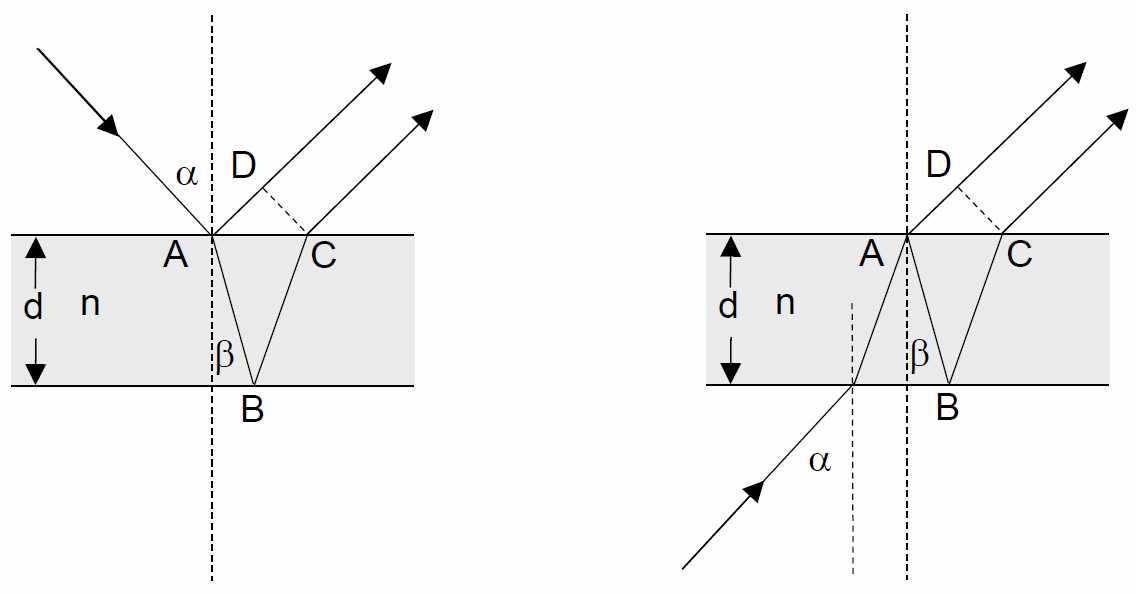
\includegraphics[width=0.6\textwidth]{Abbildungen/Glasplatten.png}\\
	\begin{tikzpicture}[scale=.9]
	\fill[fill=gray!20] (-3,-1.5) -- (3,-1.5) -- (3,0) -- (-3,0) -- (-3,-1.5);
	\draw[thick] (-3,-1.5) -- (3,-1.5);
	\draw[thick] (-3,0) -- (3,0);
	\draw[dashed] (0,-3.5) -- (0,2);
	\draw[thick] (-2,2) -- (0,0);
	\draw[->,thick] (-1.1,1.1) -- (-1,1);
	\draw[<->,thick] (-2.5,0) -- (-2.5,-1.5);
	\draw[thick,->] (0,0) -- (2,2);
	\draw[thick,->] (1,0) -- (2.5,1.5);
	\draw[dashed] (1,0) -- (0.5,0.5) node[anchor=south east, xshift=3pt] {D};
	\draw[thick] (0,0) node[anchor=north east] {A} --(0.5,-1.5) node[below] {B} -- (1,0) node[anchor=north west] {C};
	\node at (-0.25, 0.5) {$\alpha$};
	\node at (0.2, -1.25) {$\beta$};
	\node at (-1.5, -0.75) {n};
	\node at (-2.7, -0.75) {d};
	\end{tikzpicture}\hspace{2cm}
	\begin{tikzpicture}[scale=.9]
	\fill[fill=gray!20] (-3,-1.5) -- (3,-1.5) -- (3,0) -- (-3,0) -- (-3,-1.5);
	\draw[thick] (-3,-1.5) -- (3,-1.5);
	\draw[thick] (-3,0) -- (3,0);
	\draw[dashed] (0,-3.5) -- (0,2);
	\draw[thick] (-2.75,-3.5) -- (-0.75,-1.5) -- (0,0);
	\draw[dashed] (-0.75,-3.5) -- (-0.75,-0.75);
	\draw[->,thick] (-2.75,-3.5) -- (-1.75,-2.5);
	\draw[<->,thick] (-2.5,0) -- (-2.5,-1.5);
	\draw[thick,->] (0,0) -- (2,2);
	\draw[thick,->] (1,0) -- (2.5,1.5);
	\draw[dashed] (1,0) -- (0.5,0.5) node[anchor=south east, xshift=3pt] {D};
	\draw[thick] (0,0) node[anchor=north east, xshift=-3pt] {A} --(0.5,-1.5) node[below] {B} -- (1,0) node[anchor=north west] {C};
	\node at (-1.5, -0.75) {n};
	\node at (-2.7, -0.75) {d};
	\node at (0.2, -1.25) {$\beta$};
	\node at (-1.1, -2.25) {$\alpha$};
	\end{tikzpicture}
\end{center}

\subsubsection{Reflexion}

\begin{enumerate}[(1)]
	\item Länge der Wege $ \ol{AB} $ und $ \ol{BC} $
	\begin{equation*}
	x_{AB} = \frac{d}{\cos \beta} \quad x_{BC} = \frac{d}{\cos \beta}
	\end{equation*}
	\item Weg $ \ol{AD} $
	\begin{equation*}
	x_{AD} = \ol{AC} \sin \alpha = 2 d \tan \beta \sin \alpha
	\end{equation*}
	\item Gangunterschied
	\begin{equation*}
	x = n \left(x_{AB} + x _{BC}\right) - x_{AD}
	\end{equation*}
	$ n $: Brechungsindex der Glasplatte\\
	mit $ \sin \alpha = n \sin \beta $ gilt:
	\begin{equation*}
	x = 2 d n \cos \beta = 2 d \sqrt{n^2 - \sin^2 \alpha}
	\end{equation*}
	\item Phasenunterschied\\
	Phasenunterschied aufgrund des Gangunterschieds $ \Delta \varphi = kx = \frac{2\pi}{\lambda} x $\\
	$ \approx $ senkrechter Einfall:\\
	Phasensprung um $ \pi $ bei der Reflexion am optisch dichteren Medium \color{red!75!black} \mau \color{black}\\
	\lcom{Bei senkrechtem Einfall, bei der Reflexion an einem optisch dichteren Medium, tritt
	ein Phasensprung um $ \pi $ auf (dies ergibt sich aus den Randbedingungen siehe z.B. ExpII, ist
	ähnlich zur Reflexion an ,,harter`` Oberfläche, siehe ExpI)}
	\begin{equation*}
	\Rightarrow \Delta \varphi = k x  + \pi
	\end{equation*}
	\item Für konstruktive Interferenz (Maxima): $ \Delta \varphi = m 2 \pi $
	\begin{equation*}
	\Rightarrow \qquad 2 d \sqrt{n^2 - \sin^2 \alpha} = \left(m + \frac{1}{2}\right) \lambda
	\end{equation*}
\end{enumerate}

\subsubsection{Transmission}

\begin{enumerate}[(1)]
	\item Gangunterschied wie zuvor
	\begin{equation*}
	x = n (x_{AB} + x_{BC}) - x_{AD} = 2 d \sqrt{n^2 - \sin^2 \alpha}
	\end{equation*}
	\item Phasenunterschied\\
	Gangunterschied $ \Rightarrow \Delta \varphi = kx $\\
	Phasensprünge $ \Rightarrow 0 $
	\begin{equation*}
	\Rightarrow \qquad \Delta \varphi = kx
	\end{equation*}
	\item Maxima:
	\begin{equation*}
	\Rightarrow \qquad 2d\sqrt{n^2 - \sin^2 \alpha} = m \lambda
	\end{equation*}
\end{enumerate}
\textbf{Test:}\\
Annahme: keine Absorption in der Glasplatte: \lcom{Die Intensitäten der Reflexion und die der Streuung sollten sich zu Gesamtintensität aufsummieren. }
\begin{equation*}
\Rightarrow \tx{ zu erwarten: } \quad I = I_{\tx{reflektiert}} + I_{\tx{transmittiert}}
\end{equation*}
Wie erwartet da wo die Transmission maximal ist ist die Reflexion minimal und umgekehrt. Immer um $ \frac{\lambda}{2} $ verschoben.
\subsubsection{Anwendung}
\begin{itemize}
	\item \versuch{Interferenz mit zwei angewinkelten Spiegeln Fres'nelscher Doppelspiegel}
	\folie{Fres'nelscher Doppelspiegel}
	\item \folie{Newton's Ringe}
	\item \versuch{Seifenblase} die in Regenbogenfarben schillert
	\item \versuch{Interferenz an Planparalleler Folie} (mit grünem Laserlicht demonstriert)
\end{itemize}

\subsection{Vielstahlinterferenz, Fabry-P\'erot-Interferometer}

\folie{Vielstrahlinterferenz an Planparallelen Platten}
\begin{center}
	\centering
	%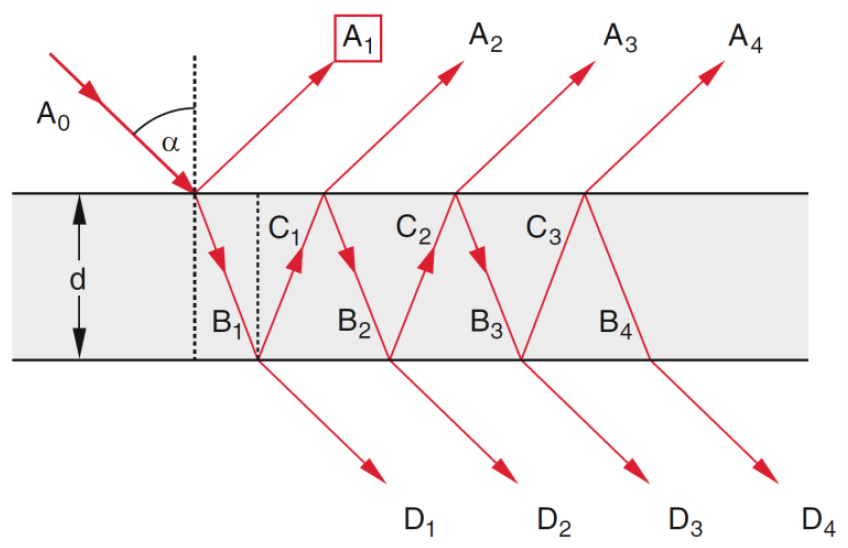
\includegraphics[width=0.6\textwidth]{Abbildungen/Glasplatten2.png}\\
	\begin{tikzpicture}[scale=1.3]
	\fill[fill=gray!20] (-2,-1.5) -- (5,-1.5) -- (5,0) -- (-2,0) -- (-2,-1.5);
	\draw[thick] (-2,-1.5) -- (5,-1.5);
	\draw[thick] (-2,0) -- (5,0);
	\node at (-1.7, -0.75) {d};
	\draw[<->,thick] (-1.5,0) -- (-1.5,-1.5);
	\draw[dashed] (0,2) -- (0,-1.5);
	\node at (-0.25, 0.5) {$\alpha$};
	\pgfsetcolor{red!80!black}
	\draw[thick] (-1.5,1.5) -- (0,0);
	\draw[->,thick] (-1.1,1.1) -- (-1,1);
	%
	\draw[thick, ->] (0,0) -- (0.5,-1.5) node[anchor=south east,black] {$B_1$} -- (1,0) node[anchor=north east,black] {$C_1$} -- (1.5,-1.5) node[anchor=south east,black] {$B_2$} -- (2,0) node[anchor=north east,black] {$C_2$} -- (2.5,-1.5) node[anchor=south east,black] {$B_3$} -- (3,0) node[anchor=north east,black] {$C_3$} -- (3.5,-1.5) node[anchor=south east,black] {$B_4$} -- (4.5,-2.5) node[anchor=north west,black] {$D_4$};
	\draw[->,thick] (2.5,-1.5) -- (3.5,-2.5) node[anchor=north west,black] {$D_3$};
	\draw[->,thick] (1.5,-1.5) -- (2.5,-2.5) node[anchor=north west,black] {$D_2$};
	\draw[->,thick] (0.5,-1.5) -- (1.5,-2.5) node[anchor=north west,black] {$D_1$};
	%
	\draw[->,thick] (3,0) -- (4,1) node[anchor=south west,black] {$A_4$};
	\draw[->,thick] (2,0) -- (3,1) node[anchor=south west,black] {$A_3$};
	\draw[->,thick] (1,0) -- (2,1) node[anchor=south west,black] {$A_2$};
	\draw[->,thick] (0,0) -- (1,1) node[anchor=south west,black] {$A_1$};
	%
	\draw[->,thick] (0,0) -- (0.25,-0.75);
	\draw[->,thick] (1,0) -- (1.25,-0.75);
	\draw[->,thick] (2,0) -- (2.25,-0.75);
	\draw[->,thick] (3,0) -- (3.25,-0.75);
	%
	\draw[->,thick] (0.5,-1.5) -- (0.75,-0.75);
	\draw[->,thick] (1.5,-1.5) -- (1.75,-0.75);
	\draw[->,thick] (2.5,-1.5) -- (2.75,-0.75);
	\end{tikzpicture}
\end{center}
\lcom{Die Interferenz ähnelt der bei einem Gitter. Der große Unterschied liegt darin, dass die Intensität der Teilstrahlen mit zunehmenden Reflexionen abnimmt. }\\
Reflexion (Transmission aus $ I = I_{\tx{ref}} + I_{\tx{trans}} $)
\begin{enumerate}[(1)]
	\item Intensitäten der jeweiligen Teilstrahlen berücksichtigen\\
	$ \Rightarrow $ Reflexionskoeffizient $ R $
	\begin{align*}
	|A_1| &= \sqrt{R} |A_0|\\
	|B_1| &= \sqrt{1 - R} |A_0|\\
	|D_1| &= \sqrt{1-R} |B_1| = (1-R) |A_0|\\
	|C_1| &= \sqrt{R} |B_1| = \sqrt{R}\sqrt{1 - R} |A_0|\\[7pt]
	|A_2| &= \sqrt{1 - R} |C_1|\\
	|B_2| &= \sqrt{R} |C_1| = R \sqrt{1 - R} |A_0|
	\end{align*}
	Einsetzen liefert\\
	$\Rightarrow \quad |A_{m+1}| = \sqrt{1-R} |C_m| = \sqrt{1-R} \sqrt{R} |B_m| = \sqrt{1-R} \sqrt{R} \sqrt{R} |C_{m-1}| = R |A_m|$
	\vspace{5pt}
	\begin{equation*}
	\Rightarrow \qquad |A_{m+1}| = R |A_m| \qquad |D_{m+1}| = R |D_m|
	\end{equation*}
	\item Gangunterschied benachbarter Strahlen (siehe Platte)
	\begin{equation*}
	x = 2d \sqrt{n^2 - \sin^2 \alpha} 
	\end{equation*}
	\item Phasenunterschied
	\begin{equation*}
	\Delta \varphi = \custo{\leftarrow}{kx}{\mathclap{\tx{Gangunterschied}}} + \tx{Phasensprünge}
	\end{equation*}
	Bei den Phasensprüngen folgt nach längerer Arbeit, dass nur der Phasensprung $ A_1 $ übrig bleibt.
	\item Gesamtamplitude
	\begin{equation*}
	A = \color{red} \pm \color{black} \sum_{m=1}^{N} A_m e^{i(m-1) \Delta \varphi}
	\end{equation*}
	$ N $: Anzahl der betrachteten Teilstrahlen\\
	$ \color{red} \pm \color{black} $: Berücksichtigt die Phasensprünge
	\item Grenzübergang $ N \to \infty $ (unendlich lange Glasplatte):
	\begin{equation*}
	\Rightarrow \qquad A = \pm A_0 \sqrt{R} \frac{1 - e^{i \Delta \varphi}}{1 - R e^{i \Delta \varphi}}
	\end{equation*}
	\begin{equation*}
	\Rightarrow \rmbox{I_R = |A^2| = 2 I_0 R \frac{1 - \cos \Delta \varphi}{1 - 2 R \cos \Delta \varphi + R^2}}
	\end{equation*}
\end{enumerate}

\subsubsection{Ergebnis}

\begin{center}
	\begin{minipage}{.6\linewidth}
		\frbox{Airy-Formeln}{
			\begin{equation*}
			I_R = I_0 \frac{F \sin^2 \left(\frac{\Delta \varphi}{2}\right)}{1 + F \sin^2\left(\frac{\Delta \varphi}{2}\right)}
			\end{equation*}
			\begin{equation*}
			I_T = I_0 \frac{1}{1 + F \sin^2 \left(\frac{\Delta \varphi}{2}\right)}
			\end{equation*}
		}
	\end{minipage}
\end{center}
\begin{equation*}
F = \frac{4 R}{(1-R)^2} \qquad \frac{\Delta \varphi}{2} = 2 \pi \frac{d}{\lambda} \sqrt{n^2 - \sin^2 \alpha}
\end{equation*}
\emph{Beispiel:} \textbf{senkrechter Einfall}
\begin{equation*}
\Rightarrow \alpha = 0 \qquad I_T = I_0 \frac{1}{1 + F \sin^2 (n d k)}
\end{equation*}
wobei $ k = \frac{2 \pi}{\lambda} $
Maxima: $$ 2 n d = m \lambda $$
FWHM (full width at half maximum)
$$ \epsilon = 4 \arcsin\sqrt{\frac{1}{F}} \approx \frac{4}{\sqrt{F}} $$
$ \Rightarrow \quad  R \to 1 \ \Leftrightarrow $ schmal-bandige Maxima\\
\folie{Maxima beim FWHM}\\[5pt]
\textbf{Anwendung: Fabry-P\'erot-Interferometer}\\
\folie{zu Fabry-P\'erot-Interferometern}\\[5pt]
\versuch{Natrium-Dampf-Lampe Interferenz}
\folie{Interferenz mit einer Natrium-Dampf-Lampe}\\[5pt]
\versuch{Abpumpen der Luft beim Interferenzmuster der Natrium-Dampf-Lampe}
\lcom{Das Muster verändert sich erheblich obwohl der Unterschied der Brechungsindizes so gering war. Also hat das Farbinterferometer eine sehr hohe Auflösung. }

% Vorlesung %20.11.18

\section{Interferenz und Beugung II - Huygen'sches Prinzip}

\subsection{Huygen'sches Prinzip}

\rbox{Jeder Punkt einer Wellenfront ist Ausgangspunkt einer neuen Elementarwelle.}
\noindent
\emph{Beispiel:} \textbf{Brechung}\\
Erklärung über Ausbreitung ebener Wellen \folie{Brechung mit Ebenen Wellen}
%
%
%
% Bild von Folie
%
%
%
\subsection{Interferenz am Doppelspalt}

Jeder Spalt, wenn er klein genug ist, wird als ,,Sender`` einer Elementarwelle angesehen.\\
$ \Rightarrow $ Überlagerung von zwei Kugelwellen.\\
\folie{zu Doppelspalt mit Kugelwellen}
%
%
%
% Bild von Folie einfügen
%
%
%
\subsection{Beugung}

Beugung bezeichnet das Phänomen, das Licht (und andere Wellen) in Bereiche vordringt, in welche es als Strahl betrachtet nicht vordringen dürfte.\\
\lcom{Beugung tritt immer an Stellen auf, an denen die Transmission einer Welle verhindert wird. Dies ist z.B. der Fall an Kanten bei denen an einer Seite komplette Abschattung und an der anderen komplette Transmission stattfindet.}\\
\lcom{Interferenz tritt dann auf, wenn es zwei solche Stellen gibt an denen Beugung auftritt.}\\
\versuch{Laser mit Kante und später Loch-/Kreisblende und später Stecknadelkopf}
\lcom{Man sieht auch ein dieser einzelnen Kante Interferenz. Dies zu verstehen ist Ziel der heutigen Vorlesung. \textbf{Das Interferenzmuster ist die Fouriertransformation einer Stufenfunktion.} Bei der Lochblende einer Fouriertransformation eines ,,Loches``.}\\
\folie{Doppelspalt Beugung} \folie{Einzelspalt}\\

\subsection{Allgemeine Behandlung der Beugung}

\lcom{Zur Verallgemeinerung Behandeln wir nun das Kirchhoff'sche Beugungsintegral.}

\subsubsection{Kirchhoff'sches Beugungsintegral}

\lcom{In verschiedenen Büchern treten häufig andere Formel des Gleichen Integrals auf.}\\
\folie{Beugungsintegral}\\
\lcom{Die Blende wird als eine Transmissionsfunktion beschrieben. Zu jedem Punkt aus dem Schirm gibt es dann ein Integral der Intensitäten aller Elementarwellen aus der Blende.}
%
%
%
% Bild einfügen
%
%
%
\noindent
Blendenöffnung bei $ z = 0 $\\
Beobachtungsschirm bei $ z = z' = z_0 $
\frbox{Kirchhoff'sches Beugungsintegral}{
\begin{equation*}
\vec{E}(\vec{x}') = \frac{ik}{2 \pi} \int Q \tau(x,y) \vec{E}_{\tx{ein}} (\vec{x}) \frac{e^{-ikr}}{r} \dd \sigma 
\end{equation*}}

\noindent
$ Q \defeq $ Neigungsfaktor\\
$ \tau \; \defeq $ Transmissionsfunktion mit $ \left\{ \begin{array}{ll}
\tau = 1 : & \tx{vollständige Transmission} \\ \tau = 0 : & \tx{undürchlässig}
\end{array} \right. $\\
$ r \ \defeq $ Abstand des Punkts $ \vec{x} $ und $ \vec{x}' $
\begin{equation*}
r^2 = (\vec{x} - \vec{x}')^2 = (x-x')^2 + (y-y')^2 + z'^2
\end{equation*}
\textbf{Sketch der Herleitung}
\begin{enumerate}[(1)]
	\item Für das von der Blende bei $ z = 0 $ durchgelassene Licht gilt:
	\begin{equation*}
	E_{\tx{Blende}} (x,y) = E_{\tx{ein}} (x,y,z=0) e^{i\varphi (x,y,z=0)}
	\end{equation*}
	\item Jeder Punkt der Öffnung erzeugt eine Elementarwelle
	\begin{equation*}
	\dd E(x',y',z') \propto Q \tau(x,y) E_{\tx{ein}} (x,y) \frac{e^{-ikr}}{r} \ub{\dd x \dd y}_{d\sigma}
	\end{equation*}
	\begin{equation*}
	Q \propto \frac{1}{2} (\cos \theta_1 + \cos \theta)
	\end{equation*}
	\item Insgesamt:
	\begin{equation*}
	E(x,y',z') \propto \int Q \tau(x,y) E_{\tx{ein}} \frac{e^{-ikr}}{r} \dd \sigma
	\end{equation*}
	\item  Vektoren und Beträge ,,richtig```machen.
\end{enumerate}
\textbf{Grenzfälle:}
\begin{itemize}
	\item Frauenhofer-Beugung:\\
	Abstand des Schirms von der Blende sehr groß gegenüber Öffnung der Blende.
	\begin{equation*}
	z' \gg x,y \qquad z_0 \gg \frac{b^2}{\lambda}
	\end{equation*}
	\item Fresnel Beugung:\\
	Abstand des Schirms von Blende klein.
	\begin{equation*}
	z' \ll x,y \qquad z_0 \ll \frac{b^2}{\lambda}
	\end{equation*}
	\item Überganszone $ z_0 \approx \frac{b^2}{\lambda} $
\end{itemize}
\folie{Folie Nah-/Übergangs-/Fernbereich}

\subsection{Allgemeines Ergebnis für die Beugung im Fernbereich, Frauenhofer Beugung}

Fernbereich: $ z' \gg x,y $
\begin{equation*}
r = \sqrt{(x-x')^2 + (y-y')^2 + z'^2}
\end{equation*}
\lcom{Zur Näherung: Näherungen zu machen ist nicht sehr einfach und der Prozess nicht sehr präzise zu Beschreiben. Es ist nicht leicht eine gute Näherung zu finden. Man muss dabei darauf Achten, dass man durch seine Näherung nicht interessante physikalische Zusammenhänge ,,Wegnähert``. In unserem Fall muss die $ e $-Funktion genau genähert werden, das r im Nenner nur grob.}\\
präziser Nähern wir $ z' \gg \frac{1}{\lambda} (x^2 + y^2) $
\begin{equation*}
r \approx z' \left(1 - \frac{xx'}{z'^2} - \frac{yy'}{z'^2} + \frac{x'^2 + y'^2}{2 z'^2}\right)
\end{equation*}
Im Nenner $ r \approx z' $\\
In dieser Näherung auch $ Q \approx 1 $

\subsubsection{Beugungsintegral für Frauenhofer Beugung}

Nebenrechnung: $ \frac{e^{-ikr}}{r} \approx \frac{e^{-ikz'}}{z'} e^{ik\frac{x'}{z'}x} e^{ik\frac{y'}{z'}y} e^{-ik \frac{1}{2 z'} (x'^2 + y'^2)} $\\
Die ersten Beiden Faktoren hiervon landen später im Vorfaktor $ A $.
\begin{equation*}
\vec{E}(\vec{x}') = \ub{A(\vec{x}')}_{\mathclap{\substack{\tx{alles Lästige} \\ \tx{geht dort rein}}}} \int \tau(x,y) \vec{E}_{\tx{ein}}(x,y) e^{i k \frac{x'}{z'} x} e^{ik\frac{y'}{z'}y} \dd x \dd y
\end{equation*}
2D Fourier Integral:
\begin{equation*}
\vec{F} (u,v) \equiv \int \tau(x,y) \vec{E}_{\tx{ein}} (x,y) e^{iux} e^{ivy} \dd x \dd y
\end{equation*}
\frbox{Beugungsintegral für Frauenhofer Beugung}{
\begin{equation*}
\Rightarrow \quad \vec{E}(\vec{x}') = A(\vec{x}') \vec{F} \left(k \frac{x'}{z'} , k \frac{y'}{z'}\right)
\end{equation*}}
\noindent
\emph{Beispiel:} \textbf{Einfachspalt}
\begin{align*}
\tx{Ortsraum} \qquad &\Leftrightarrow \qquad \tx{Fourier Raum}\\
\tau(x,y) = \casess{1}{\forall  \frac{-b}{2} \le x \le \frac{b}{2}}{0}{\tx{sonst.}} \qquad &\Leftrightarrow \qquad \vec{F}(k) = \frac{\sin x}{x} \qquad x = \frac{\pi}{b} k \frac{x'}{z'}\\
\tx{schmaler/breiter Spalt} \qquad &\Leftrightarrow \qquad \tx{breites/schmales Interferenzmuster}
\end{align*}
\begin{equation*}
\Delta x \Delta h < \const
\end{equation*}

\subsection{Auflösungsvermögen optischer Instrumente}

\lcom{Es ist Wichtig zu Wissen von welcher Art von Vergrößerung geredet wird. Welche wir hier benutzen wird später genauer erklärt.}

\subsubsection{Lochkurven}

\folie{Zu Lochkurven und Darstellung mit Lochblenden}\\
\versuch{Darstellung von Dia mit Lochblende}

\subsubsection{Rayleigh Kriterium}

\rbox{Zwei Punkte sind gerade dann noch unterscheidbar, wenn das Beugungsmaximum des einen Punktes in das 1.-te Beugungsminimum des anderen Punktes fällt.}
\noindent
\folie{Auflösung: Überlagerung von Beugungsmustern}\\
\lcom{Diese Definition ist nichts eindeutiges. Es ist nur eine Möglichkeit an einem Breiten Übergang von Scharf bis Unscharf.}

\subsubsection{Ein anderes Kriterium}
Abstand der Hauptmaxima muss größer sein als deren Halbwertsbreite.

% Vorlesung %21.11.18

\subsection{Räumliches Auflösungsvermögen}

\emph{Beispiel:} \textbf{Linse}\\
\folie{Zu Bündelung von Licht mit einer Linse}\\[5pt]
\versuch{Laser: Beugung an der Doppellochplatte}
\lcom{Je näher die Löcher in der Blende zueinander rücken, desto ausgeprägter wird das Interferenzmuster.}\\
Beugung an einer Lochblende:\\
1. Maximum:
\begin{equation*}
r \sin \alpha = 0{,}61 \lambda
\end{equation*}
\textbf{Auflösung einer Lochblende}
\begin{equation*}
\Rightarrow \quad \sin \alpha_{\tx{min}} = 1{,}22 \frac{\lambda}{D}
\end{equation*}
$ D: $ Durchmesser des Lochs\\[5pt]
\textbf{Auflösung einer Linse}
\begin{equation*}
\Rightarrow \quad \sin \alpha_{\tx{min}} = 1{,}22 \frac{\lambda}{D}
\end{equation*}
$ D: $ Durchmesser der Linse\\[5pt]
\textbf{Auflösung eines Fernrohrs}\\
Das durch das Objektiv erzeugte Zwischenbild ist bereits beugungsverbreitert.
\begin{equation*}
\Rightarrow \quad \sin \alpha_{\tx{min}} = 1{,}22 \frac{\lambda}{D}
\end{equation*}
$ D: $ Durchmesser des Objektivs\\[5pt]
\textbf{Auflösung eines Mikroskops}\\
Im Unterschied zu vorher ist das einfallende Licht nicht parallel.\\
\folie{zur Auflösung am Mikroskop}
\begin{enumerate}[(1)]
	\item mit der Kleinwinkelnäherung gilt:
	\begin{equation*}
	d = b \alpha_{\tx{min}}
	\end{equation*}
	\begin{align*}
	\Rightarrow \alpha_{\tx{min}} &= 1{,}22 \frac{\lambda}{D} \\
	\Rightarrow \quad \: \, d &= 1{,}22 \frac{b \lambda}{D}
	\end{align*}
	$ D: $ Durchmesser des Objektivs
	\item Für den Abstand $ \delta_x $ \textbf{vor} dem Objektiv gilt
	\begin{equation*}
	\delta_x \approx \frac{f_1}{b} d = 1{,}22 \frac{f_1 \lambda}{D}
	\end{equation*}
	\item Öffnungswinkel $ \varphi $
	\begin{equation*}
	\sin \varphi \approx \frac{D}{2 f_1}
	\end{equation*}
\end{enumerate}
\begin{center}
	\begin{minipage}{.5\linewidth}
		\frbox{Auflösung eines Mikroskop}{
		\begin{equation*}
		\delta_x \approx 0{,}61 \, \frac{\lambda}{n \sin\varphi}
		\end{equation*}	
		}
	\end{minipage}
\end{center}
$ n \sin \varphi : $ numerische Apertur\\
\lcom{Der \textbf{Gültigkeitsbereich der Formel} ist der \textbf{Fernbereich} (Frauenhofer Beugung). Wir versuchen Bessere Ergebnisse zu erzielen indem wir Situationen Betrachten, die außerhalb dieses Gültigkeitsbereichs liegen.}\\
\lcom{Warum tritt der Faktor $ \sin \varphi $ auf? Dies ergibt sich einsichtig aus Abbe's Theorie: Zwei Punkte senden interferierende Kugelwellen aus (siehe Doppelspalt), wobei mindestens das 1.te Nebenmaximum vom Objektiv noch erfasst werden muss, um ein Bild entstehen zu lassen. Daher:}
\begin{equation*}
\tx{1.tes Nebenmaximum: } \sin \alpha = \frac{\alpha}{\delta_x} \Rightarrow \sin \varphi \approx \sin \alpha \Rightarrow \delta_x \approx \frac{\lambda}{\sin \varphi}
\end{equation*}

\noindent
\textbf{Verbesserungen} der beugungsbegrenzten Auflösung:
\begin{itemize}
	\item kleines $ \lambda $
	\begin{itemize}
		\item[$ \rightarrow $] Elektronenmikroskop ($ 1 \, \tx{nm} $)
		\item[$ \rightarrow $] Röntgen (in Entwicklung)
	\end{itemize}
	\item Immersionsöl mit Brechungsindex von $ n \approx 1{,}5 $
	\item Nahfeldmikroskopie\\
	Die obigen Überlegungen basieren auf der Frauenhofer Beugung. \lcom{ In diesem Fall nutzen wir die Nahfeld Mikroskopie, wo die Fresnel'sche Beugung auftritt und wir darüber eine höhere Auflösung erzielen können.}
\end{itemize}

\noindent
\lcom{Was im nächtes Kapitel nicht behandelt wird. Polarisation,Doppelbrechung ,nichtlineare optik}

\chapter{Licht - Materie Wechselwirkung}

\section{lineare und zirkulare Polarisation}

EM-Welle
\begin{equation*}
\Rightarrow \vec{E},\vec{B},\vec{k}
\end{equation*}
\textbf{Definition: } Polarisation $ \widehat{=} $ Richtung von $ \vec{E} $\\
transversale Wellen: $ \ \vec{E} \perp \vec{k} \quad \Leftrightarrow \quad \ \: \vec{E} \cdot \vec{k} = 0 $\\
longitudinale Wellen: $ \vec{E} \parallel \vec{k} \, \quad \Leftrightarrow \quad \vec{E} \times \vec{k} = 0 \quad \Leftrightarrow \quad \left(\vec{E} \cdot \vec{k}\right) \vec{k} = \vec{k}^2 \vec{E} $\\
\lcom{Für die Behauptung, dass EM-Wellen Transversalwellen haben wir die Annahme getroffen, dass wir uns im Vakuum befinden. In Materie ist die Ausbreitungsgeschwindigkeit kleiner als $ c $ und der $ \vec{k} $-Vektor hat eine Komponente parallel zur Ausbreitungsrichtung. $ \Rightarrow $ longitudinale EM-Wellen (eigentlich keine EM-Wellen sondern anderer Name).}\\
zur Vereinfachung nehmen wir an $ \Rightarrow \vec{k} = (0,0,k) $

\subsection{Lineare Polarisation}

\folie{linear polarisierte EM-Welle}
\begin{equation*}
\vec{E} = \ub{E_0 \begin{pmatrix}
\cos \tilde{\varphi} \\ \sin \tilde{\varphi} \\ 0
\end{pmatrix}}_{\vec{E}_0} \cos \left(\omega t - k z + \varphi \right)
\end{equation*}
\emph{Bemerkung:}
\begin{itemize}
	\item Die zwei Polarisationsrichtungen schwingen \textbf{in Phase}.
	\item nur für die linear polarisierte ebene Welle kann der ,,Polarisationsanteil`` $ \vec{E}_0 $ vom ,,Ausbreitungsanteil`` $ \cos (\omega t - \vec{k} \vec{z} + \varphi) $ ab separiert werden
\end{itemize}

\subsection{Zirklulare Polarisation}

\folie{zirkular polarisierte EM-Welle}
\begin{equation*}
\vec{E} = E_0 \begin{pmatrix}
\cos \left(\omega t - kz + \varphi \right) \\ \pm\sin\left(\omega t - k z + \varphi\right) \\ 0
\end{pmatrix}
\end{equation*}
\emph{Bemerkung:}
\begin{itemize}
	\item die zwei Polarisationsrichtungen schwingen um $ \frac{\pi}{2} $ \textbf{Phasen verschoben}, aber haben gleiche Amplitude
\end{itemize}

\subsection{Zusammenhang zwischen linear und zirkular polarisierten Wellen}

\rbox{Jede linear polarisierte Welle kann in zwei entgegengesetzt zirkular polarisierte Wellen halber Amplitude zerlegt werden und umgekehrt.}
\noindent
\emph{Beispiel:} Zerlegung von linearer in zirkulare Polarisation.
$ \cos\left( x + \frac{\pi}{2}\right) + \cos\left( x - \frac{\pi}{2}\right) = 0 $
\begin{align*}
\vec{E}(\vec{x},t) &= A \begin{pmatrix}
\cos\left(\omega t - k z + \varphi\right) \\ 0 \\ 0
\end{pmatrix} \\
&= \frac{A}{2} \begin{pmatrix}
\cos\left(\omega t - k z + \varphi \right) \\ \cos\left(\omega t - k z + \varphi + \frac{\pi}{2}\right) \\ 0
\end{pmatrix} + \frac{A}{2} \begin{pmatrix}
\cos \left(\omega t - k z + \varphi\right) \\ \cos \left(\omega t -  k z + \varphi - \frac{\pi}{2}\right) \\ 0
\end{pmatrix}
\end{align*}

\subsection{Elliptische Polarisation}

Die Spitze des $ \vec{E} $-Feldvektors bewegt sich mit der Frequenz $ \omega $ auf einer Ellipse
\begin{equation*}
\vec{E} = \begin{pmatrix}
E_x \cos(\omega t - k z + \varphi) \\
E_y \cos(\omega t - k z + \varphi \pm \frac{\pi}{2}) \\
0
\end{pmatrix}
\end{equation*}
\emph{Bemerkung:}
\begin{itemize}
	\item die zwei Polarisationsrichtungen schwingen um $ \frac{\pi}{2} $ Phase verschoben UND haben unterschiedliche Amplituden
\end{itemize}

\subsection{Polarisation beim Durchgang durch Materie}

\subsubsection{Doppelbrechung:}

\begin{equation*}
k_x \neq k_y
\end{equation*}
\begin{equation*}
\vec{E}(\vec{x},t) = \begin{pmatrix}
A_x \cos\left(\omega t - \color{black!30!red}k_x\color{black}z + \varphi_x\right) \\ A_y \cos\left(\omega t - \color{black!30!red}k_y\color{black}z + \varphi_y \right) \\ 0
\end{pmatrix}
\end{equation*}

\subsubsection{optische Aktivität}

Die Ausbreitungsgeschwindigkeit bzw. der Wellenvektor für rechts und links zirkulare Polarisation unterschiedlich.

\begin{align*}
\Rightarrow \quad \vec{E}(\vec{x},t) &= \frac{A}{2} \begin{pmatrix}
\cos\left(\omega t - \color{black!30!red}k^+\color{black}z + \varphi\right) \\ \cos\left(\omega t -\color{black!30!red}k^+\color{black}z + \varphi + \frac{\pi}{2}\right) \\ 0
\end{pmatrix} + \frac{A}{2} \begin{pmatrix}
\cos\left(\omega t - \color{black!30!red}k^-\color{black}z + \varphi\right) \\ \cos\left(\omega t - \color{black!30!red}k^-\color{black}z+\varphi-\frac{\pi}{2}\right) \\ 0
\end{pmatrix}\\
&=A \begin{pmatrix}
\cos\left(\delta kz\right) \\ \sin\left(\delta kz\right) \\ 0
\end{pmatrix} \cos\left(\omega t - \overline{k}z + \varphi\right)
\end{align*}
\begin{equation*}
k^+ = \overline{k} + \delta k \qquad k^- = \overline{k} - \delta k
\end{equation*}

\section{Polarisation durch Brechung und Reflexion}

(siehe EX II)

\subsection{Maxwell Gleichungen in Materie}

\begin{equation*}
\tx{div} \vec{D} = \rho_0 \qquad \qquad \tx{div} \vec{B} = 0 \qquad \qquad
\end{equation*}
\begin{equation*}
\tx{rot} \vec{E} = - \prt{}{t} \vec{B} \qquad \tx{rot} \vec{H} = \vec{j}_0 + \prt{}{t} \vec{D}
\end{equation*}
plus:
\begin{align*}
\vec{F} &= q \left(\vec{v} \times \vec{B}\right) \\
\vec{F} &= q \vec{E}
\end{align*}
\begin{equation*}
\rho = \rho_0 + \rho_{\tx{pol}} \equiv \frac{1}{\epsilon} \rho_0 \qquad \vec{j} = \vec{j}_0 + \vec{j}_{\tx{mag}} \equiv \mu \vec{j}_0
\end{equation*}
Es fehlen hier noch einige Zusammenhänge die selbstverständlich immer noch gelten z.B.:
\begin{equation*}
\tx{div} \vec{E} = \frac{1}{\epsilon_0} \rho \qquad \tx{rot} \vec{B} = \mu_0 \vec{j} + \frac{1}{c^2} \prt{}{t} \vec{E} 
\end{equation*}
\begin{equation*}
\vec{D} = \epsilon_0 \vec{E} + \vec{P} \qquad \vec{B} = \mu_0\left(\vec{H} + \vec{M}\right)
\end{equation*}
alle sechs Felder: $\vec D  \vec E \vec P \ \ \vec M \vec H \vec B$ jeweils Maxwell-Gleichungen\\
plus:
\begin{equation*}
\tx{Materialgleichungen z.B.:} \quad \vec{D} (\vec{E}) \ , \ \vec{P}(\vec{E}) \ , \dots
\end{equation*}

\subsection{Erinnerung: Polarisation bei Brechung und Reflexion}

\folie{Brechung und Reflexion bei parallelem und orthogonalem $ \vec{E} $-Feld in der Einfallsebene}\\
\folie{Einfallswinkel und Reflexionswinkel (Brewsterwinkel)}

\subsubsection{Physikalische Ursache: Stetigkeits \& Randbedingungen}

Gewöhnliche partielle Diff-Gleichungen
\begin{enumerate}[$ \Rightarrow $]
	\item viele Lösungen
	\item Anfangsbed, Randbed., Stetigkeitsbed.
\end{enumerate}
\begin{minipage}{.6\linewidth}
	\emph{Beispiele:}
	\begin{itemize}
		\item Metall:
		Randbedingung aus Elektrostatik überlegt 
		\item Ein- und Ausschaltvorgänge bei RLC Gleichungen
		Anfang: Schalter offen, Spule ,,aufgeladen``
		\begin{equation*}
		\Rightarrow I = \frac{U}{(R_i + R)}
		\end{equation*}
		Dann: Schalter schließen $ \Rightarrow U = 0 $
		$ \Rightarrow $ wie verhält sich aber $ I , U_{\tx{Spule}}, \dots $ ?\\
		Energie der Spule ist stetig $ \ \ E_{\tx{Spule}} = \frac{1}{2} L I^2 $
		\begin{equation*}
		\Rightarrow I_{\tx{Spule}} \tx{ stetig}
		\end{equation*}
	\end{itemize}
\end{minipage}%
\begin{minipage}{.4\linewidth}
	\centering
	%t1:
	\begin{tikzpicture}
	\centerarc[pattern = north east lines](0,0)(200:90:2cm);
	\draw[very thick,->] (135:2cm) -- node[anchor=south west] {$ \vec{E} $} ++(135:1.2cm);
	\centerarc[](135:2cm)(135:40:.3cm);
	\node[fill=black,circle,inner sep=.5pt,minimum size=.5pt] at ($ (135:2cm) + (.01,.15) $) {};
	\draw[white] (0,0) -- (0,-1.2);
	\end{tikzpicture}
	%t2:
	%\draw[decoration={aspect=0.3, segment length=3mm, amplitude=3mm,coil},decorate] (-2,0)--(a);
	\begin{tikzpicture}
	\coordinate (u) at (0,0);
	\coordinate (r1) at (1,1.5);
	\coordinate (r2) at (3.5,1.25);
	\coordinate (l) at (3.5,-.25);
	\coordinate (s) at (2.5,.5);
	\draw[thick] ($ (u) + (-.5,.1) $) -- ++(1,0);
	\draw[thick] ($ (u) + (-.4,-.1) $) -- ++(.8,0);
	\draw[thick] ($ (r1) + (0,-.2) $) rectangle node[] {$ R_i $} ($ (r1) + (1,.2) $);
	\draw[thick] ($ (r2) + (-.2,0) $) rectangle node[] {$ R $} ($ (r2) + (.2,-1) $);
	\draw[decoration={aspect=0.5, segment length=2mm, amplitude=2mm,coil},decorate,thick] (l) -- node[right=10pt] {$ L $} ($ (l) + (0,-1) $);
	\node[circle,fill=black,inner sep=1pt,minimum size=1pt] at (s) {};
	\node[circle,fill=black,inner sep=1pt,minimum size=1pt] at ($ (s) + (0,-1) $) {};
	\draw ($ (u) + (0,.11) $) -- (0,1.5) -- (r1);
	\draw ($ (r1) + (1,0) $) -- (3.5,1.5) -- (r2);
	\draw ($ (r2) + (0,-1) $) -- (l);
	\draw ($ (l) + (0,-1) $) -- (3.5,-1.5) -- (0,-1.5) -- ($ (u) + (0,-.1) $);
	\draw ($ (s) + (0,1) $) -- (s);
	\draw ($ (s) + (0,-2) $) -- ($ (s) + (0,-1) $) -- ++(135:1.2cm);
	\node at (-1,0) {$ U $};
	\end{tikzpicture}
\end{minipage}%

% Vorlesung 27.11.18

\subsection{Maxwell-Gleichungen und Stetigkeitsbedingungen}

\lcom{Heute beschäftigen wir uns mit Stetigkeitsbedingungen. Diese sind sehr Wichtig für die Lösung von Differentialgleichungen zur Lösung von Randwertproblemen.}
\begin{comment}% old Version
\begin{align*}
\tx{div} \vec{D} = \rho_0 \quad &\Rightarrow \quad \left(\vec{D}_2 - \vec{D}_1\right) \cdot \vec{n} = \sigma_{\tx{Fläche}}\\[5pt]
\tx{div} \vec{B} = 0 \quad &\Rightarrow \quad \left(\vec{B}_2 - \vec{B}_1\right) \cdot \vec{n} = 0\\
\tx{rot} \vec{E} = - \prt{}{t} \vec{B} \quad &\Rightarrow \quad \left(\vec{E}_2 - \vec{E}_1\right) \times \vec{n} = 0\\
\tx{rot} \vec{H} = \vec{j}_0 + \prt{}{t} \vec{D} \quad &\Rightarrow \quad \left(\vec{H}_2 - \vec{H}_1\right) \times \vec{n} = \vec{j}_{\tx{Fläche}}
\end{align*}
\end{comment}
\begin{equation*}
\begin{split}
&\tx{div} \vec{D} = \rho_0 \\[8pt]
&\tx{div} \vec{B} = 0 \\
&\tx{rot} \vec{E} = - \prt{}{t} \vec{B} \\
&\tx{rot} \vec{H} = \vec{j}_0 + \prt{}{t} \vec{D}
\end{split}
\begin{split}
\quad \Rightarrow \quad \\[8pt]
\quad \Rightarrow \quad \\[8pt]
\quad \Rightarrow \quad \\[8pt]
\quad \Rightarrow \quad 
\end{split}
\begin{split}
\left(\vec{D}_2 - \vec{D}_1\right) \, \cdot \, \vec{n} &= \sigma_{\tx{Fläche}} \\[8pt]
\left(\vec{B}_2 - \vec{B}_1\right) \, \cdot \, \vec{n} &= 0 \\[8pt]
\left(\vec{E}_2 - \vec{E}_1\right) \times \vec{n} &= 0 \\[8pt]
\left(\vec{H}_2 - \vec{H}_1\right) \times \vec{n} &= \vec{j}_{\tx{Fläche}}
\end{split}
\end{equation*}
\begin{enumerate}[$ \Rightarrow $]
	\item Normalkomponenten von $ \vec{B}(\vec{x},t) $ ist stetig
	\item Tangentialkomponente von $ \vec{E}(\vec{x},t) $ ist stetig
\end{enumerate}
\textbf{(nahezu) senkrechten Einfall}\\
$ \alpha,\beta \approx 0 $\\

\begin{minipage}{.05\linewidth}
	$ \perp : $ \\\\[5pt] $ \parallel : $
\end{minipage}%
\begin{minipage}{.45\linewidth}
	\centering
	Reflexion
	\begin{equation*}
	E_{\tx{ref} \perp} = - E_{\tx{ein} \perp} \frac{n_2 - n_1}{n_2 + n_1}
	\end{equation*}
	\begin{equation*}
	\phantom{-} \, E_{\tx{ref} \parallel} = \phantom{-} E_{\tx{ein} \parallel} \, \frac{n_2 - n_1}{n_2 + n_1} \ \ \,
	\end{equation*}
	\vspace{10pt}
\end{minipage}\nolinebreak%
\begin{minipage}{.45\linewidth}
	\centering
	Transmission
	\begin{equation*}
	E_{\tx{trans} \perp} = E_{\tx{ein} \perp} \frac{2 n_1}{n_2 + n_1}
	\end{equation*}
	\begin{equation*}
	E_{\tx{trans} \parallel} = E_{\tx{ein} \parallel} \frac{2 n_1}{n_2 + n_1}
	\end{equation*}
	\vspace{10pt}
\end{minipage}%
\\
Betrachtung für senkrechten Einfall\\
\folie{Stetigkeitsbed. bei senkrechtem Einfall}
\begin{enumerate}[(1)]
	\item $ \perp $ und $ \parallel $ sind identisch $ \Rightarrow $ wähle $ \perp $
	\item Aus Stetigkeit der Tangentialkomponenten von $ E $
	\begin{equation*}
	E_{I} = E_{II}
	\end{equation*}
	\begin{equation*}
	\Rightarrow \qquad E_{\tx{ein} \perp} + E_{\tx{ref} \perp} = E_{\tx{trans} \perp}
	\end{equation*}
	(aus Gauß Zylinder folgt die Gleichheit der E Felder auf einer Seite mit dem E Feld auf der anderen Seite)
	\item Stetigkeit des Energieflusses\\
	\folie{Stetigkeits an Randflächen}
	\begin{equation*}
	\Rightarrow \qquad I_{\tx{ein}} = I_{\tx{ref}} + I_{\tx{trans}}
	\end{equation*}
	\item $ I = n c_0 \epsilon_0 E^2 $
	\begin{equation*}
	\Rightarrow \qquad n_1 (E_{\tx{ein} \perp})^2 = n_1 (E_{\tx{ref} \perp})^2 + n_2 (E_{\tx{trans} \perp})^2
	\end{equation*}
\end{enumerate}
$ \Rightarrow $ Lösungen wie oben

\subsection{Warum war es ,,erlaubt`` mit ebenen Wellen zu rechnen ?}

\begin{enumerate}[(1)]
	\item Lösungen im homogenen Raum, Raum kann begrenzt sein
	\item Grenzfälle $ \rightarrow $ Lösungen in den jeweiligen Teilräumen, wurden durch Stetigkeitsbed. angeschlossen.
	\item Maxwell-Gleichungen sind linear $ \leftrightarrow $ Superpositionsprinzip.\\[5pt]
	spezielle Lösung:
	\begin{equation*}
	\vec{E}(\vec{x},t) = \vec{E}_0 e^{i(\vec{k} \vec{x} - \omega t)} \qquad \tx{ mit } \omega(\vec{k})
	\end{equation*}
	$ \vec{k} $ als Parameter zum ,,numerieren`` der Lösungen\\[5pt]
	allgemeine Lösung:
	\begin{eqnarray}
	\vec{E}(\vec{x},t) = \int \vec{E}_0(\vec{k}) e^{i(\vec{k} \vec{x} - \omega(\vec{k}) t)} \dd \vec{k}
	\end{eqnarray}
\end{enumerate}
$ \Rightarrow $ Allgemein:
\begin{equation*}
\vec{E}_I(\vec{x}_{\tx{Grenzfläche}},t) = \vec{E}_{II} (\vec{x}_{\tx{Grenzfläche}},t)
\end{equation*}
speziell:
\begin{equation*}
\vec{E}(\vec{x},t,p)
\end{equation*}
allgemein:
\begin{equation*}
\vec{E}(\vec{x},t) = \int \vec{f}(p) \vec{E}(\vec{x},t,p) \dd p
\end{equation*}

\section{Maxwell-Gl. in Materie, komplexer Brechungsindex}

\begin{equation*}
\tx{\lcom{\mau \ Im folgenden Kapitel tauchen oft $ \mu $ und $ \epsilon $ auf. Gemeint sind hier aber oft $ \mu_r $ und $ \epsilon_r $ \mau}}
\end{equation*}
Vereinfachung: $ \mu = 1 \ \tx{ eigentlich } \ \mu_r \qquad \vec{B} = \mu_o \vec{H} $

\subsection{Polarisation eines Dielektrikums}

\textbf{phänomenologisch/makroskopisch:}
\begin{equation*}
\vec{D} = \epsilon_0 \vec{E} + \vec{P}
\end{equation*}
allgemein gültig, bis auf:
\lcom{Die Einschränkung der Maxwellgleichungen in Materie sind nur Mittlungen des Mikroskopische Bildes in eine fast Makroskopischen Bereich. Daraus ergibt sich die Einschränkung: Wenn unser Beobachtungsbereich zu klein wird, sind diese Mittlungen nicht mehr gültig.}
\begin{equation*}
\vec{P} = \epsilon_0 \overset{\circ}{\chi} \vec{E} + \dots
\end{equation*}
häufig gültig\\[5pt]
lineare, isotrope Medien
\begin{equation*}
\vec{D} = \epsilon_0 \vec{E} + \vec{P} = \epsilon_0 \epsilon \vec{E} \qquad \vec{P} = \epsilon_0 \chi \vec{E} = \epsilon_0 (\epsilon - 1) \vec{E}
\end{equation*}
$ \chi : $ dielektrische Suszeptibilität $ \chi_e = (\epsilon - 1) \ \tx{ eigentlich } \ = (\epsilon_r - 1) $\\[5pt]
mikroskopisch:
\begin{equation*}
\vec{d} = \alpha \vec{E}
\end{equation*}
$ \vec{d} : $ induziertes Dipolmoment\\
$ \alpha : $ Polarisierbarkeit

\subsection{Ensemble unabhängiger induzierter Dipolmomente}

\begin{equation*}
\vec{P} = \frac{1}{V} \sum_i \vec{d}_i \quad \rightarrow \quad \frac{N}{V} \vec{d} \quad \tx{da sich alle Objekte gleich verhalten}
\end{equation*}
\begin{equation*}
\rightarrow \qquad \chi = \frac{1}{\epsilon_0} \frac{N}{V} \alpha \quad \equiv \epsilon - 1 \ (\epsilon_r - 1)
\end{equation*}
\lcom{Gilt bei Gasen gut, bei Festkörpern aufgrund von Dipol-Dipol-Wechselwirkungen nicht mehr gut.}

\subsection{Lorenz-Lorentz-Oszillatormodell}

\folie{Lorenz-Lorentz-Oszillatormodell für die Polarisation}
\begin{equation*}
\Rightarrow \quad \hat{\epsilon} = \epsilon' + i \epsilon''
\end{equation*}
\lcom{Im Mitschrieb steht hier mehr zum Thema}

\subsection{Wellengleichung in Materie}

Materie $ \Rightarrow \rho \neq 0 $
\begin{equation*}
\Rightarrow \quad \tx{div} \vec{E} \neq 0
\end{equation*}
$ \Rightarrow $ Aus $ \tx{div} \vec{E} = 0 $ folgte das eine EM-Welle im Vakuum transversal sind. Dies muss  also nicht mehr so sein.\\[5pt]
Unter Verwendung von
\begin{enumerate}[(1)]
	\item \begin{equation*}
	\tx{rot rot} \vec{E} \custoup{\rightarrow}{=}{\mathclap{\tx{MW}}} - \prt{}{t} \tx{rot} \vec{B} \custoup{\rightarrow}{=}{\mathclap{\mu = 1}} - \mu_0 \prt{}{t} \tx{rot} \vec{H} \custoup{\rightarrow}{=}{\mathclap{\tx{MW}}} - \mu_0 \prt{^2}{t^2} \vec{D}
	\end{equation*}
	\item \begin{equation*}
	\tx{rot rot} \vec{E} = - \vabla^2 \vec{E} + \tx{grad div} \vec{E}
	\end{equation*}
\end{enumerate}
\begin{equation*}
\Rightarrow \qquad \rmbox{\vabla^2 \vec{E} - \frac{1}{c_0^2} \prt{^2}{t^2} \frac{\vec{D}}{\epsilon_0} - \tx{grad div} \vec{E} = 0}
\end{equation*}
\color{black!20!red} $ \tx{grad div} \vec{E} $ ist wegen $ \tx{div} \vec{E} \neq 0 $ \color{black}

\subsection{Wellengleichung in Materie in komplexer Schreibweise}
\begin{equation*}
\hat{\vec{D}} = \epsilon_0 \hat{\epsilon} \hat{\vec{E}} \qquad \hat{\epsilon} = \epsilon' + i \epsilon''
\end{equation*}
\begin{equation*}
\Rightarrow \qquad \vabla^2 \vec{E} - \frac{1}{c_0} \hat{\epsilon} \prt{^2}{t^2} \vec{E} - \tx{grad div} \vec{E} = 0
\end{equation*}
\begin{enumerate}[(1)]
	\item Einsetzen:
	\begin{equation*}
	\vec{E} = \hat{\vec{E}}_0 \tx{exp} \left[i (\hat{\vec{k}} \vec{x} - \omega t)\right] \qquad \hat{\vec{k}} = \vec{k}' + i \vec{k}''
	\end{equation*}
	\item Ausführen der Differentiale
	\begin{equation*}
	\tx{div} \vec{E} = \begin{pmatrix}
	\prt{}{x} \\ \prt{}{y} \\ \prt{}{z}
	\end{pmatrix} \cdot \hat{\vec{E}}_0 e^{i(\hat{\vec{k}} \vec{x} - \omega t)} = \begin{pmatrix}
	i \hat{k}_x \\ i \hat{k}_y \\ i \hat{k}_z
	\end{pmatrix} \cdot \hat{\vec{E}}_0 e^{i(\hat{\vec{k}} \vec{x - \omega t})} 
	\end{equation*}
	und kürzen des Phasenfaktors
	\begin{align*}
	\tx{div} \vec{E} \quad &\rightarrow \quad i \hat{\vec{k}} \cdot \hat{\vec{E}}_0 \\
	\tx{rot} \vec{E} \quad &\rightarrow \quad i \hat{\vec{k}} \times \hat{\vec{E}}_0 \\
	\vabla^2 \vec{E} \quad &\rightarrow \quad - \left(\hat{\vec{k}} \cdot \hat{\vec{k}}\right) \hat{\vec{E}}_0 \\
	\tx{grad} (\tx{div} \vec{E}) \quad &\rightarrow \quad - \left(\hat{\vec{k}} \cdot \hat{\vec{E}}_0\right) \hat{\vec{k}}\\
	\prt{^2}{t^2} \vec{E} \quad &\rightarrow \quad - \omega^2 \hat{\vec{E}}_0
	\end{align*}
	\item Lösung
	\begin{equation*}
	\Rightarrow \qquad \rmbox{- \left(\hat{\vec{k}}^2\right) \hat{\vec{E}}_0 + \frac{\omega^2}{c_0^2} \hat{\epsilon} \hat{\vec{E}}_0 + \left(\hat{\vec{k}} \cdot \hat{\vec{E}}_0\right) \hat{\vec{k}} = 0 }
	\end{equation*}
\end{enumerate}
Beachte:\\
$ \hat{\vec{k}}^2 $ ist \textbf{nicht} das Betragsquadrat
\begin{equation*}
\hat{\vec{k}}^2 = \vec{k}'^2 - \vec{k}''^2 + 2 i \vec{k}' \cdot \vec{k}''
\end{equation*}

\subsubsection{Was bedeutet $ \hat{\vec{k}} = \vec{k}' + i \vec{k}'' $ ?}

\begin{equation*}
e^{i(\hat{\vec{k}} \vec{x} - \omega t)} = e^{i \vec{k}'' \vec{x}} e^{i(\vec{k}' \vec{x} - \omega t)}
\end{equation*}
Teil mit $ \vec{k}'' : $ Dämpfung, Absorption der Welle beim Durchgang durch Materie $ I(x) = I_0 e^{-2 |k''| x} $\\
Teil mit $ \vec{k}' : $ Ausbreitung der Welle mit $ \lambda = \frac{2 \pi}{k'} $
\emph{Bemerkung:}\\
harmonischer Oszillator: $ \hat{\omega} = \omega - i \delta $\\
$ e^{i\hat{\omega t}} = e^{-\delta t} e^{-i \omega t} $\\
$ \delta $ ist die Dämpfung

\subsection{Transversale Lösungen}

transversal $ \Leftrightarrow \quad \hat{\vec{k}} \perp \hat{\vec{E}}_0 $ 
\begin{equation*}
\Rightarrow \quad \rmbox{\hat{\vec{k}} \cdot \hat{\vec{E}}_0 = 0}
\end{equation*}
\begin{equation*}
\Rightarrow \quad \hat{\vec{k}}^2 \hat{\vec{E}}_0 + \frac{\omega^2}{c_0^2} \hat{\epsilon} \hat{\vec{E}}_0 = 0
\end{equation*}
\begin{equation*}
\Rightarrow \quad \rmbox{\hat{\vec{k}}^2 = \frac{\omega^2}{c_0^2} \hat{\epsilon}}
\end{equation*}
\begin{equation*}
\Rightarrow \quad \rmbox{\omega(\hat{\vec{k}}) = c_0 \sqrt{\frac{\hat{\vec{k}}^2}{\hat{\epsilon}}}}
\end{equation*}
Real- und Imaginärteil von $ \hat{\vec{k}} $ sind verknüpft mit Real- und Imaginärteil von $ \hat{\epsilon} $

\subsection{Komplexwertiger Brechungsindex}

\begin{equation*}
\hat{n} = n + i K = \sqrt{\hat{\epsilon}}
\end{equation*}
$ n : $ Brechungsindex\\
$ K : $ Extinktionskoeffizient
\begin{align*}
\Rightarrow \quad 2 n^2 &= \sqrt{\epsilon'^2 + \epsilon''^2} + \epsilon'\\
2 K^2 &= \sqrt{\epsilon'^2 + \epsilon''^2} - \epsilon'
\end{align*}
\begin{equation*}
\Rightarrow \quad \rmbox{\sqrt{\hat{\vec{k}}^2 } = \frac{\omega}{c_0} \hat{n}}
\end{equation*}

\subsection{Lösung für kleine imaginäre Anteile. (schwache Dämpfung bzw Absorbtion)}

Im allgemeinen ist die Lösung nicht einfach, da hier die Wurzeln aus komplexen Zahlen gezogen werden. Deshalb betrachten wir hier die Lösung für kleine imaginäre Anteile.\\
$ k'' \ll k' \quad K \ll n \quad \epsilon'' \ll \epsilon' $
\begin{align*}
2n^2 &= \sqrt{\epsilon'^2 + \epsilon''^2} + \epsilon' \cong \epsilon' \left(1 + \frac{1}{2} \frac{\epsilon''^2}{\epsilon'^2}\right) + \epsilon' \approx 2 \epsilon' \\
2K^2 &= \sqrt{\epsilon'^2 + \epsilon''^2} - \epsilon' \cong \epsilon' \left(1 + \frac{1}{2} \frac{\epsilon''^2}{\epsilon'^2}\right) - \epsilon' \approx \frac{1}{2} \frac{\epsilon''^2}{\epsilon'} = \frac{1}{2} \frac{\epsilon''^2}{n^2}
\end{align*}
\begin{equation*}
\Rightarrow \quad \rmbox{n = \sqrt{\epsilon'} \qquad K = \frac{\epsilon''}{2n}}
\end{equation*}
Was den Wellenvektor angeht erhalten wir:
\begin{equation*}
\sqrt{\hat{\vec{k}}^2} = \sqrt{\vec{k}'^2 - \vec{k}''^2 + 2 i \vec{k}' \cdot \vec{k}''} \approx | \vec{k}' | + i \frac{\vec{k}' \cdot \vec{k}''}{|\vec{k}'|}
\end{equation*}
\begin{equation*}
\Rightarrow \quad |\vec{k}'|  + i \frac{\vec{k}' \cdot \vec{k}''}{|\vec{k}'|} = \frac{\omega}{c_0} (n + i K)
\end{equation*}
\textbf{Physikalische Interpretation}\\[5pt]
Der Realteil von $\epsilon'$ führt zu einer Ausbreitungsgeschwindigkeit $ c = \frac{c_0}{\sqrt{\epsilon'}} $\\
Der Imaginärteil von $\epsilon'$ führt zu einer Dämpfung/Absorption der Welle.\\
$\rightarrow$ In Materie gibt es transversale EM-Wellen mit $ c = \frac{c_0}{\sqrt{\epsilon'}}$ (falls $c\leq c_0$)

% Vorlesung 28.11.18

\subsection{Evaneszente Welle}

\subsubsection{Totalreflektion}

\folie{Evaneszente Welle}\\
$ \alpha \ge \alpha_T \Rightarrow $ keine Wellenausbreitung im optisch dünneren Medium\\[5pt]
Das bedeutet nicht, dass keine el.-mag.-Felder in diesen Bereich eindringen.\\
\folie{Felder treten in Medium ein.}\\
\lcom{Die Felder sind jedoch so schwach, dass sie nach großem Abstand nicht mehr Messbar sind. Sie klingen mit der Einhüllenden $ e^{i k''} $ ab. $ k' $ ist null, da es sich nur um EM-Felder handelt und nicht um eine sich ausbreitende Welle.}\\
\versuch{Übertragung von Evaneszenten Wellen durch zwei Prismen mit geringem Abstand.}
\textbf{Beobachtung:}\\
Die Evaneszente Welle kann ins zweite Prisma eindringen und sich dort ausbreiten.\\
\textbf{Theorie:}\\
Prisma: $ \hat{\epsilon} = \epsilon' + i \epsilon''  \qquad \epsilon' \gg \epsilon''$\\
Das Licht im Prisma wird nur schwach gedämpft. Es ist für Mikrowellen transparent so wie Glas für sichtbares Licht.\\
Vereinfachung:
\begin{equation*}
\epsilon'' = 0
\end{equation*}
Beachte: I.A. nicht $ k'' = 0 $\\[5pt]
Frage: Kann es ein $ \hat{\vec{k}} $ geben, der komplex bzw. imaginär ist?
\begin{equation*}
\hat{\vec{k}}^2 = \frac{\omega^2}{c_0^2} \epsilon' = \vec{k}'^2 - \vec{k}''^2 + 2 i \vec{k}' \cdot \vec{k}''
\end{equation*}
Für sichtbares Licht im Vakuum gilt:
\begin{equation*}
\epsilon' > 0
\end{equation*}
\begin{equation*}
\Rightarrow \quad \vec{k}'^2 - \vec{k}''^2 + 2 i \vec{k}' \cdot \vec{k}'' > 0
\end{equation*}
Lösung 1: Der Normalfall der Wellenausbreitung
\begin{equation*}
\vec{k}'' = 0
\end{equation*}
Lösung 2: Evaneszente Welle
\begin{equation*}
\vec{k}'' > 0 \ \tx{aber} \ \vec{k}' \perp \vec{k}''
\end{equation*}
\begin{equation*}
\Rightarrow \quad \vec{k}'^2 - \vec{k}''^2 > 0
\end{equation*}
\emph{Beispiel:} \textbf{Totalreflexion mit $ \beta = 90 ^\circ $}\\
$ x $-Achse in Richtung der Ausbreitung der Totalreflektierten, $ z $-Achse orthogonal dazu in Richtung des dünneren Mediums $ n_2 $,\\
\lcom{Die $ \vec{k}' $ Komponente ist bei der Totalreflexion parallel zur Oberfläche des Mediums.}\\[5pt]
\textbf{einfallende Welle:}\\
normale Ausbreitung
\begin{equation*}
\hat{\vec{k}}_1 = \vec{k}_1 + i 0
\end{equation*}
\begin{equation*}
\Rightarrow \quad k_1^2 = \frac{\omega^2}{c_0^2} n_1^2 \qquad (k_1: \tx{ Betrag von } \hat{\vec{k}}_1)
\end{equation*}
aus der Geometrie folgt:
\begin{equation*}
k_{1,x} = k_1 \sin\alpha
\end{equation*}
\begin{equation*}
\Rightarrow \quad k_{1,x}^2 = \frac{\omega^2}{c_0^2} n_1^2 \sin^2 \alpha
\end{equation*}
\textbf{ausfallende Welle:}
\begin{equation*}
\hat{\vec{k}}_2 = \begin{pmatrix}
k_{2,x} \\ 0 \\ i k_{2,z}
\end{pmatrix} \quad \Rightarrow \quad \begin{array}{c}
\vec{k}' = (k_{2,x} , 0 , 0) \\ \vec{k}'' = (0 , 0 , k_{2,z})
\end{array}
\end{equation*}
\begin{equation*}
\Rightarrow \quad \hat{\vec{k}}_2^2 = \frac{\omega^2}{c_0^2} n_2^2 = \vec{k}_2'^2 - \vec{k}_2''^2 = k_{2,x}^2 - k_{2,z}^2 > 0
\end{equation*}
\begin{equation*}
\frac{\omega^2}{c_0^2} n_2^2 = k_{2,x}^2 - k_{2,z}^2 > 0
\end{equation*}
Brechungsgesetz: $ n_1 \sin\alpha = n_2 $
\begin{equation*}
\Rightarrow \quad \custo{\leftarrow}{k_{1,x}^2}{\tx{\color{red} > 0 \color{black}}} = k_{2,x}^2 - k_{2,z}^2 \color{red} >0 \color{black}
\end{equation*}
\begin{flushright}
	\vspace{-20pt}
	\color{red} Q.E.D. \color{black}
\end{flushright}
$ \Rightarrow $ Im Falle der Totalreflexion existiert eine evaneszente Welle \mau

\section{Streuung, Spektren und Verwandtes}

\subsection{Grobe Einteilung}

Materiewelle
\begin{itemize}
	\item \textbf{reflektierend} = Licht wird \textbf{gerichtet} zurückgestrahlt
	\item \textbf{streuend} = Licht wird \textbf{ungerichtet} zurückgestrahlt
\end{itemize}
Materie ist
\begin{itemize}
	\item \textbf{absorbierend} = Licht wird \textbf{verschluckt}
	\item \textbf{durchsichtig} = Licht wird \textbf{durchgelassen}
	\item \textbf{transparent} = Licht wird \textbf{teilweise durchgelassen}, \textbf{teils absorbiert} und/oder \textbf{teil gestreut}
\end{itemize}

\subsection{Physikalische Prozesse: Grundgedanken}

\begin{enumerate}[A)]
	\item \textbf{ elastischer/inelastischer Stoß $ \rightarrow $ Streuung}\\
	\folie{zur Streuung an Teilchen}\\
	wie beim Billard\\[5pt]
	\emph{Beispiel:} Lichtstreuung, Streuung am Photon
	\begin{itemize}
		\item Rayleigh-Streuung: elastische Streuung von Photonen an gebundenen Elektronen
		\item Thomson-Streuung: elastische Streuung an ,,quasi freien`` Elektronen
		\lcom{,,quasi frei``: eventuell gebunden aber winzige Bindungsenergie im Vergleich zur Energie der einfallenden Strahlung.}
		\item Compton-Streuung: inelastische Streuung an ,,quasi freien`` Elektronen\\
		relativistisches Billard
		\item Raman-Streuung: inelastische Streuung aufgrund eines inelastischen Stoßes
		\item Mie-Streuung, Brillouin-Streuung, $ \dots $
	\end{itemize}
	\emph{Beispiel:} andere Teilchen
	\begin{itemize}
		\item Elektronenstreuung
		\item Neutronenstreuung
		\item geladene Teilchen: Rutherford-Streuung, Mott-Streuung
	\end{itemize}
	\item \textbf{Anregung/Abregung}\\
	Genereller Ablauf:\\
	\textbf{Anregung} des Systems durch Licht, Stöße oder Wärme $ \rightarrow $ \textbf{Lebensdauer der Anregung} $ \rightarrow $ \textbf{Abregung} des Systems als Licht, aussenden eines Teilchens, Wärme $ \dots $\\[5pt]
	\emph{Beispiel:}
	\begin{itemize}
		\item Absorption: ein Photon wird absorbiert
		\begin{equation*}
		\hbar \omega \rightarrow \Delta E_{\tx{System}}
		\end{equation*}
		\item spontane Emission, Luminanz
		\begin{equation*}
		\Delta E_{\tx{System}} \rightarrow \hbar \omega
		\end{equation*}
		Fluoreszenz: Lebensdauer Kurz ps bis ns \\
		Phosphoreszenz: Lebensdauer deutlich länger als ns \\
		\item Stimulierte Emission:
		\begin{equation*}
		\hbar \omega + \Delta E_{\tx{System}} \rightarrow 2 \hbar \omega
		\end{equation*}
		\lcom{Aus einem Angeregten System und einem einfallenden Photon entstehen zwei kohärente Photonen.}
		\item Photoeffekt:
		\begin{equation*}
		\hbar \omega \rightarrow E_{e^-}
		\end{equation*}
	\end{itemize}
\end{enumerate}

\subsection{Wirkungsquerschnitt (W.Q.S.)}

Üblicherweise als differentieller W.Q.S. (entspricht geometrisch einer Streuung)
\begin{equation*}
\frac{\dd^2 \sigma}{\dd \Omega \dd E}
\end{equation*}
\lcom{Der W.Q.S. ist ein maß dafür wie sehr ein System Streut.}\\
\folie{Streuung und Wirkungsquerschnitt}\\
\lcom{Hierbei wird die Kugel an der Gestreut wird in kleine Flächenelemente geteilt: Raumwinkel-Einheiten.}\\
\folie{Streuung von Teilchen an Materie (Atomen)}

\subsection{Energie und Impulserhaltung}
$ \Rightarrow $ Betrachtung im Energiediagramm\\[5pt]
häufig: System durch diskrete Energieniveaus Beschrieben.\\[5pt]
\folie{Energiediagramme Absorption und ,,dips`` im Frequenz-Intensität Diagramm}\\
\folie{Energiediagramme bei elastischer Streuung}\\
\folie{Energiediagramme bei inelastischen Streuung}\\
\folie{inelastische Streuung Vergleich von verschiedene Streuungen}\\
Streuung über Virtuelle Zustände (ein nicht diskretes Energieniveau)\\
\folie{Spontane Emission, Lumineszenz}\\
\folie{nochmal aber nicht Disskutiert}\\
\folie{Quanten dots}\\
\folie{Stimmulierte Emmision}\\
\folie{Photo Effekt} \ hier wird das Elektron in einen nicht-diskreten Zustand gehoben.\\
\folie{Up-Conversion (nicht-linearer Effekt)}\\
\folie{Grüner Laserpointer (eigentlich IR Laser und Kristall der mit Up-Conversion grünes Licht erzeugt)}\\

% Vorlesung 04.12.18 (20 days until christmas)

\subsection{Spektroskopie}

\begin{equation*}
\tx{Spektroskopie } = \tx{ Intensität vs. Frequenz}
\end{equation*}
\lcom{Ein Energiesektrum und ein gemessenes Intensitätsspektrum sind nicht das selbe! Ein Energiespektrum zeigt absolute Energieniveaus an, ein Intensitätsspektrumm Energiedifferenzen.}\\[5pt]
Typischer Aufbau:
\begin{equation*}
\tx{Quelle } \rightarrow \tx{ Probe } \rightarrow \tx{ Analysator, Detektor}
\end{equation*}
Die Quelle kann monochromatisch sein oder weißes Licht ausstrahlen (breites Spektrum von Frequenzen).\\
Die Energieanalyse ,,Richtung`` $ \prd{^2 \sigma}{E \dd \Omega} $ ($ \sigma = $ Wirkungsquerschnitt)\\
\folie{einfaches Prismen-Spektrometer}\\
\folie{ESR (Elektronen-Spin-Resonanz) Spektrometer}\\
\lcom{Beim ESP Spektrometer wird das Energiespektrum der Probe verändert (durch angelegte\\ Mag\-net\-fel\-der). Der Messstrahl wird zuerst aufgeteilt in einen Vergleichsstrahl und einen\\ Messstrahl, die vor dem Detektor wieder zusammengefügt werden um dort wir beim Michelson-Interferometer zu interferieren.}\\
\folie{ein kommerzielles Spektrometer}

\subsubsection{Typische Messkonfiguration}

\begin{itemize}
	\item Reflektionsspektrum %t1:
	\item Transmissionsspektrum %t2:
	\item Emissionsspektrum
	\item Absorptionsspektrum
\end{itemize}
\begin{center}
	\begin{tikzpicture}
		\node[circle,draw=black,line width=1pt,inner sep=2pt,minimum size=20pt] (q) at (-.9,1.4) {$ Q $};
		\node[circle,draw=black,line width=1pt,inner sep=2pt,minimum size=20pt] (p) at (.9,1.4) {$ P $};
		\node[circle,draw=black,line width=1pt,inner sep=2pt,minimum size=20pt] (d) at (0,0) {$ D $};
		\draw[thick,->] (q) -- (p);
		\draw[thick,->] (p) -- (d);
		\node[above] at (0,2) {Reflektion:};
	\end{tikzpicture}
	\hspace{2cm}
	\begin{tikzpicture}
		\node[circle,draw=black,line width=1pt,inner sep=2pt,minimum size=20pt] (q) at (-1.4,0) {$ Q $};
		\node[circle,draw=black,line width=1pt,inner sep=2pt,minimum size=20pt] (p) at (0,0) {$ P $};
		\node[circle,draw=black,line width=1pt,inner sep=2pt,minimum size=20pt] (d) at (1.4,0) {$ D $};
		\draw[thick,->] (q) -- (p);
		\draw[thick,->] (p) -- (d);
		\node[above] at (0,.7) {Transmission:};
	\end{tikzpicture}
	\hspace{2cm}
	\begin{tikzpicture}
		\node[circle,draw=black,line width=1pt,inner sep=2pt,minimum size=20pt] (q) at (-1.8,0) {$ Q $};
		\node[circle,draw=black,line width=1pt,inner sep=2pt,minimum size=20pt] (p) at (0,0) {$ P $};
		\node[circle,draw=black,line width=1pt,inner sep=2pt,minimum size=20pt] (d) at (1,-1) {$ D $};
		\draw[thick,->] (q) -- (p);
		\draw[thick,->] (p) -- (d);
		\node[above] at (-1,1) {Emission:};
		\foreach \a in {0,45,90,135,180,225,270,315}
		\draw[->] (\a:10pt) -- ++(\a:.7cm);
	\end{tikzpicture}
\end{center}
\folie{Schematisch: Spektrometer}\\[5pt]
\versuch{Natrium-Dampf-Lampe}
Das Licht aus der Natrium-Dampf-Lampe geht durch eine Glasröhre mit aufgedampftem Natrium. Diese Röhre wird nun erhitzt, sodass das Natrium verdampft.
Aufgrund der Erhitzung wird das nun Gasförmige Natrium von der Lampe angeregt und Emittiert selbst auch Licht derselben Farbe. Da dieses Licht nicht mehr gerichtet ist sondern in alle Richtungen strahlt wird die Intensität des transmittierten Lichts geringer.\\
Bei sehr hoher Temperatur ist die Absorption so stark, dass nach dem Anfangsbereich der Röhre schon das ganze Licht Absorbiert und ausgestrahlt wird.\\[5pt]
\versuch{Weißes Licht auf Salz (Natriumchlorid)}
Sichtbares Spektrum: Rot$ | $Grün.\\
Emissionsspektrum über Erhitzung ohne Weißlicht-Beleuchtung mit Gasbrenner (farbige Flamme)\\
Bei Erhitzung und Beleuchtung: Absorptionsspektrum: Rot - Gelb - Grün.\\[5pt]
\versuch{Rayleigh Strahlung}
Eine Lampe strahlt unpolarisiertes Weißes Licht aus.\\
Das an den Wassermolekülen (und Dreckrückständen im Wasser) gestreute Licht hat eine lineare Polarisation. Von den Molekülen geht eine Herz'sche Dipolstrahlung aus (Polarisation in Richtung der Antenne, Ausbreitung der Welle in der Ebene orthogonal dazu). Dies kommt daher, dass das Weiße licht nur transversal polarisierte Anteile hat keine longitudinalen. Daraus ergibt sich, welche Dipole angeregt werden, und das die Polarisation nur orthogonal zur Ausbreitung des Lichts stattfindet.\\
Die Rayleigh-Streuung ist mit $ \omega^4 $ Frequenzabhängig, es wird also blau wesentlich stärker Reflektiert als rotes Licht.es Licht. Dies erklärt den Blauen Schimmer um die Weiße Kreisscheibe auf dem Schirm.\\
Beim hinzugeben von winzigen Kügelchen, die im Wasser schwimmen, wird mehr Licht gestreut. Die Kreisscheibe wird immer röter und röter zunächst gelb dann dunkel orange wie die Abendsonne. Die blauen Frequenzen sind eher am Rand zu sehen und konzentrierter als zuvor. (Beim blauen Himmel sehen wir den Emissionsanteil hier den Transmissionsanteil).\\[5pt]

\subsubsection{Typen von Spektren}

Linienspektrum \& kontinuierliches Spektrum\\
\folie{verschiedene Spektren}\\
\textbf{Zugängliche Infos im Linienspektrum (Prüfungsrelevant!)}
\begin{enumerate}[1)]
	\item Die Lage des Peaks oder die Frequenz des Peaks gibt die \textbf{Übergangsenergie} an die nur eine Energiedifferenz angibt.\\
	\begin{minipage}{.8\linewidth}
		\begin{equation*}
		E_2 - E_1 = kv
		\end{equation*}
	\end{minipage}%
	\begin{minipage}{.2\linewidth}
		%t3:
		\centering
		\begin{tikzpicture}[scale=.6]
			\draw (-1,1) -- (1,1) node[right] {$ E_2 $};
			\draw (-1,-1) -- (1,-1) node[right] {$ E_1 $};
			\draw[thick,->] (0,-1) -- (0,1);
		\end{tikzpicture}
	\end{minipage}%
	\item \textbf{Intensität}: Diese hängt von der Übergangswahrscheinlichkeit und damit auch der Teilchendichte zusammen.\\
	Die Intensität hat auch mit der \textbf{stärke der Wechselwirkung} von dem Eingestrahlten (\textbf{Sonde}) mit dem Bestrahlten (\textbf{Probe}) zu tun.
	\item \textbf{Linienbreite/Linienform:}	Bei der Lorenzverteilung ist die Breite der Verteilung verknüpft mit der Lebensdauer der Teilchen.
	\begin{equation*}
	e^{-\frac{t}{\tau}} \quad \Rightarrow \quad \tx{Lorenzlinie} \quad \Rightarrow \quad \tx{Lebensdauer}
	\end{equation*}
	\folie{Gaußverteilung als Summe der Wahrscheinlichkeitsverteilungen einzelner Moleküle}
	\begin{equation*}
	\tx{statistische Verteilung } \quad \Rightarrow \quad \tx{Gaußverteilung}
	\end{equation*}
\end{enumerate}

\section*{Fragerunde}
\addcontentsline{toc}{section}{IV. \texorpdfstring{\ \: }{space}  Fragerunde}

\textbf{Dispersionsrelation bei getriebener Schwingung:}\\
(harmonischer Oszillator oder Dispersion bei Schwingungen)\\
Gleichschwingung bei geringer Antriebsfrequenz.\\
Phasenverschiebung bei zu schnellem Antrieb und geringe Amplitude des Schwingers\\
quasi ein Tiefpass.\\
Dieses Problem ist mit komplexen Größen Lösbar. Zur Physikalischen Betrachtung der Lösung: Leistungsaufnahme des Schwingenden Systems. Diese Leistung ist mit dem Imaginärteil verknüpft.\\
Bei unserem Beispiel eines dielektrischen Materials geht es um Absorption. Diese stammt aus dem Leistungsverlust aus dem Imaginärteil der Dielektrizitätskonstante. Der Realteil ist hier mit dem Brechungsindex verknüpft.\\[5pt]
\textbf{Angeregte Emissionen:}\\
Das anregende und das angeregte Photon können aber müssen nicht in Phase sein. Allgemein ist dies nicht so.\\
Das angeregte Atom bleibt mit einer gewissen, statistisch verteilten Lebensdauer in dem Zustand. Wie die Anregung erfolgt ist (Stöße oder Absorption von Strahlung) ist egal. Daraus resultiert spontane Emission.\\
Die \textbf{stimulierte oder induzierte Emission} (erzeugt durch ein Strahlungsfeld) erzeugt die Abstrahlung von Photonen in Phase mit den eingestrahlten Photonen. Die Begründung ist recht kompliziert und kann nur über Quantenmechanik erfolgen.\\[5pt]
\textbf{Evaneszente Welle:}\\
Undurchdringbarkeit ist nur eine Näherung. Kein Wechsel des Mediums ist eine echte Stufenfunktion (im mikroskopischen Bereich).

% Vorlesung 5.12.18 (19 days untis christmas)

\section{Ratengleichungen}

\subsection{Exponentieller Zerfall}

\begin{equation*}
\prd{}{t} n(t) = - \frac{1}{\tau} [n(t) - n_{eq} ]
\end{equation*}
\lcom{Statistisch unabhängige Prozesse. Egal wie viele Objekte es gibt nach der Halbwertszeit ist nur noch die Hälfte da. Die einzelnen Objekte verhalten sich also unabhängig voneinander so.}\\
$ \tau : $ Radiationszeit, Zerfallszeit, Lebensdauer, Halbwertszeit, \dots\\
\textbf{Lösung:}
\begin{equation*}
n(t) = [n(o) - n_{eq}] e^{-\frac{t - t_0}{\tau}} + n_{eq}
\end{equation*}

\subsection{Zwei-Niveausystem}

\begin{center}
	%t1:
	\begin{tikzpicture}
		\coordinate (u) at ($ (0,0) + (0,1) $);
		\coordinate (d) at ($ (0,0) + (0,-1) $);
		\draw ($ (u) + (-1.5,0) $) node[left] {1} -- ++(3,0) node[right] {$ E_1 $};
		\draw ($ (d) + (-1.5,0) $) node[left] {0} -- ++(3,0) node[right] {$ E_0 $};
		\draw[red,thick,->] ($ (d) - (.5,0) $) to[out=110,in=-110] node[left] {$ \Gamma_{0\to1} $} ($ (u) - (.5,0) $);
		\draw[red,thick,->] ($ (u) + (.5,0) $) to[out=-70,in=70] node[right] {$ \Gamma_{1\to0} $} ($ (d) + (.5,0) $);
		\node[black!40!green] at ($ (u) + (2.5,0) $) {$ n_1 $};
		\node[black!40!green] at ($ (d) + (2.5,0) $) {$ n_0 $};
		\node[right,black!40!green] at (2.2,0) {Besetzungszahlen};
	\end{tikzpicture}
\end{center}
\emph{Bemerkung:}
\begin{itemize}
	\item oft gibt es eine \textbf{Zwangsbedingung} $ \sum_k n_k = N \quad N : $ Gesamtzahl der Zustände
	\item Prinzip des detaillierten Gleichgewichts
	\begin{equation*}
	\Gamma_{k \to l} = \Gamma_{l \to k}
	\end{equation*}
\end{itemize}
Ratengleichung:
\begin{equation*}
\dot{n}_0 = - \Gamma_{0 \to 1} n_0 + \Gamma_{1 \to 0} n_1
\end{equation*}
\begin{equation*}
\dot{n}_1 = - \Gamma_{1 \to 0} n_1 + \Gamma_{0 \to 1} n_0
\end{equation*}
Definition Gleichgewicht
\begin{align*}
\Rightarrow \quad \dot{n}_0 &= - \Gamma(n_0 - n_1) \\
\dot{n}_1 &= - \Gamma (n_1 - n_0)
\end{align*}
konstante Gesamtbesetzung
\begin{equation*}
n_0 + n_1 = N
\end{equation*}
\textbf{Lösung:}
\begin{align*}
\delta N \equiv n_1 - n_0 \qquad \rightarrow \quad n_0 &= \frac{1}{2} (N - \delta N) \\
n_1 &= \frac{1}{2} (N + \delta N)
\end{align*}
\begin{equation*}
\Rightarrow \quad - \frac{1}{2} \delta \dot{N} = \Gamma \delta N
\end{equation*}
\begin{equation*}
\delta N(t) = \delta N(0) e^{-\frac{t}{\tau}}
\end{equation*}

\subsubsection{Rantengleichung mit externen Stimuli}

\begin{minipage}{.5\linewidth}
	\begin{align*}
	\Rightarrow \quad \dot{n}_0 &= - \Gamma_{n_0} + \Gamma_{n_1} + \Gamma_{0 \tx{ext}}\\
	\dot{n}_1 &= - \Gamma_{n_1} + \Gamma_{n_0} + \Gamma_{1 \tx{ext}}
	\end{align*}
\end{minipage}%
\begin{minipage}{.5\linewidth}
	%t2:
	\centering
	\begin{tikzpicture}
		\coordinate (u) at ($ (0,0) + (0,1) $);
		\coordinate (d) at ($ (0,0) + (0,-1) $);
		\draw ($ (u) + (-1.5,0) $) node[left] {1} -- ++(3,0) node[right] {$ n_1 $};
		\draw ($ (d) + (-1.5,0) $) node[left] {0} -- ++(3,0) node[right] {$ n_0 $};
		\draw[red,thick,->] ($ (d) - (.5,0) $) to[out=110,in=-110] node[left] {$ \Gamma_{0\to1} $} ($ (u) - (.5,0) $);
		\draw[red,thick,->] ($ (u) + (.5,0) $) to[out=-70,in=70] node[right] {$ \Gamma_{1\to0} $} ($ (d) + (.5,0) $);
		\draw[<-] ($ (u) + (1.25,0) $) to[out=60,in=180] (2.5,2) node[right] {$ \Gamma_{1\tx{ ext}} $};
		\draw[<-] ($ (d) + (1.25,0) $) to[out=-60,in=180] (2.5,-2) node[right] {$ \Gamma_{0\tx{ ext}} $};
	\end{tikzpicture}
\end{minipage}%

\subsection{Zwei-Niveau System im Strahlungsfeld, Einstein Parameter}

\begin{minipage}{.5\linewidth}
	Im Folgenden Betrachten wir stets ein Zwei-Niveau-System wie hier in der Abbildung zu sehen ist:
\end{minipage}%
\begin{minipage}{.5\linewidth}
	%t3:
	\centering
	\begin{tikzpicture}
		\coordinate (u) at ($ (0,0) + (0,.8) $);
		\coordinate (d) at ($ (0,0) + (0,-.8) $);
		\draw ($ (u) + (-1.5,0) $) node[left] {1} -- ++(3,0) node[right] {$ E_1 , n_1 $};
		\draw ($ (d) + (-1.5,0) $) node[left] {0} -- ++(3,0) node[right] {$ E_0 , n_0 $};
	\end{tikzpicture}
\end{minipage}%
\\[15pt]
\textbf{spontane Emission:}\\
\begin{minipage}{.5\linewidth}
	\begin{align*}
	\Rightarrow \quad \dot{n}_1 &= - A_{1 \to 0} n_1 \\
	\dot{n}_0 &= + A_{1 \to 0} n_1
	\end{align*}
\end{minipage}%
\begin{minipage}{.5\linewidth}
	%t4:
	\centering
	\begin{tikzpicture}
		\coordinate (u) at ($ (0,0) + (0,.8) $);
		\coordinate (d) at ($ (0,0) + (0,-.8) $);
		\draw ($ (u) + (-1.5,0) $) -- ++(3,0);
		\draw ($ (d) + (-1.5,0) $) -- ++(3,0);
		\draw[red,thick,->] (u) -- (d);
		\draw[red,thick,->,decorate,decoration=snake] (0.5,0) -- (2.2,0) node[right] {$ h \nu $};
	\end{tikzpicture}
\end{minipage}%
\\[15pt]
\textbf{Photon Absorption:}\\
\begin{minipage}{.5\linewidth}
	\begin{align*}
	\Rightarrow \quad \dot{n}_0 &= - B_{0 \to 1} \rho(\nu) n_0 \\
	\dot{n}_1 &= + B_{0 \to 1} \rho(\nu) n_0
	\end{align*}
\end{minipage}%
\begin{minipage}{.5\linewidth}
	%t5:
	\centering
	\begin{tikzpicture}
		% ugly invisibe alignment line
		\draw[white] (0,0) -- (4.1,0);
		\coordinate (u) at ($ (0,0) + (0,.8) $);
		\coordinate (d) at ($ (0,0) + (0,-.8) $);
		\draw ($ (u) + (-1.5,0) $) -- ++(3,0);
		\draw ($ (d) + (-1.5,0) $) -- ++(3,0);
		\draw[red,thick,->] (d) -- (u);
		\draw[red,thick,->,decorate,decoration=snake] (-2.7,0) -- (-1,0) node[right] {$ h \nu $};
	\end{tikzpicture}
\end{minipage}%
\\[15pt]
$ \rho(\nu) : $ Dichte des Strahlungsfeldes\\
$ \nu : $ Frequenz\\[5pt]
\textbf{stimulierte Emission:}\\
\begin{minipage}{.5\linewidth}
	\begin{align*}
	\Rightarrow \quad \dot{n}_0 &= + B_{1 \to 0} \rho(\nu) n_1 \\
	\dot{n}_1 &= - B_{1 \to 0} \rho(\nu) n_1
	\end{align*}
\end{minipage}%
\begin{minipage}{.5\linewidth}
	%t6:
	\centering
	\begin{tikzpicture}
		% ugly invisibe alignment line
		\draw[white] (0,0) -- (3.2,0);
		\coordinate (u) at ($ (0,0) + (0,1) $);
		\coordinate (d) at ($ (0,0) + (0,-1) $);
		\draw ($ (u) + (-1.5,0) $) -- ++(3,0);
		\draw ($ (d) + (-1.5,0) $) -- ++(3,0);
		\draw[red,thick,->] (u) -- (d);
		\draw[red,thick,->,decorate,decoration=snake] (-1.8,0) -- node[above] {$ h \nu $} (-.1,0);
		\draw[red,thick,->,decorate,decoration=snake] (0.1,.4) -- (1.8,.4);
		\draw[red,thick,->,decorate,decoration=snake] (0.1,-.4) -- (1.8,-.4) node[right,yshift=12pt] {$ h \nu $};
	\end{tikzpicture}
\end{minipage}%
\\[15pt]
\textbf{Definition Gleichgewicht}
$ n_0 : $
\begin{equation*}
A_{1 \to 0} n_1 - B_{0 \to 1} \rho(\nu) n_0 + B_{1 \to 0} \rho(\nu) n_1 = 0
\end{equation*}
Thermodynamik, Quantenstatistik:
\begin{equation*}
\frac{n_k}{N} = \frac{1}{Z} e^{-\frac{E_k}{k_B T}}
\end{equation*}
\begin{equation*}
\rho(\nu) = \frac{8 \pi h \nu^3}{c^3} \frac{1}{e^{\frac{h \nu}{k_B T}} - 1}
\end{equation*}
$ Z : = \sum_k e^{-\frac{E_k}{k_B T}} $ die Zustandssumme\\
$ k_B : $ Boltzmann-Konstante\\[5pt]
$ \Rightarrow $ Planck'sches Strahlungsgesetz

\chapter{Entwicklung der Atom- und Quantenphysik}

\section{Quantelung von Masse und Ladung}

\subsection{Quantelung der Masse}

\textbf{Chemie:}\\
Dalton'sches Gesetz der multiples Proportionen\\
Satz von Avogadro\\[5pt]
$ \Rightarrow $ Dalton'sche Atomhypothese\\
$ \Rightarrow $ Periodensystem der Elemente\\[5pt]
Periodizität festgestellt durch Atomvolumen. Erst später Ionisationsenergie (Abspaltung des am schwächsten gebundenen Elektron).\\[5pt]
\textbf{Physik:}\\
kinetische Gastheorie (vor allem Maxwell)\\
Gas $ = $ Teilchen mit nur kinetischer Energie, WW mit einem Gefäß
\begin{equation*}
\Rightarrow \quad P = \frac{N}{V} m \frac{\ol{v}^2}{3}
\end{equation*}
Äquipartitionstheorem
\begin{equation*}
\ol{E_{\tx{kin}}} = \frac{3}{2} k_B T \qquad (\tx{einatomiges Gas, } f = 3)
\end{equation*}
\begin{equation*}
\Rightarrow \quad \rmbox{P V = N_A k_B T} \qquad \tx{ideale Gas Gleichung}
\end{equation*}
$ V : $ Molvolumen\\
$ \Rightarrow $ Größe der Atome\\[5pt]
\emph{Beispiel:} \textbf{Messung der Gaskonstanten $ R $ über Schallgeschwindigkeit\\}
\begin{equation*}
c^2 = \frac{f + 2}{f} R \frac{T}{M} 
\end{equation*}
\folie{Versuchsaufbau zur Messung der Gaskonstante $ R $}

\subsubsection{Direkter Nachweis über die Rastertunnelmikroskopie}

Ein Elektron, das von einem in den anderen Energiezustand springt:
\begin{center}
	%t7:
	\begin{tikzpicture}[scale=.75]
		\draw (-4,0) -| (-1.4,-2) -- (1.4,-2) |- (4,0);
		\node[circle,fill=blue,inner sep=1pt,minimum size=1pt] (e) at (-.6,-2) {};
		\node[circle,fill=blue,inner sep=1pt,minimum size=1pt] (e2) at (-2,0) {};
		\draw[->,looseness=1.5] (e) to[out=90,in=45] (e2);
		\node[blue,anchor=south west] at (e) {$ e^- $};
		\draw[thick,black!40!green,<->] (2,0) -- node[right] {Austrittsarbeit $ \Phi $} (2,-2);
		\node[red] at (0,1) {innerhalb};
		\node[red] at (-3,1) {außerhalb};
		\node[red] at (3,1) {außerhalb};
	\end{tikzpicture}
\end{center}
\vspace{10pt}
Schematische Skizze eines Rastertunnelmikroskops:
\begin{center}
	%t8:
	\begin{tikzpicture}
		\coordinate (s) at (0,.5);
		% dreieck
		\draw[thick,pattern=north east lines,rounded corners=2pt] ($ (s) + (-.5,1.5) $) -- (s) -- ($ (s) + (.5,1.5) $);
		\coordinate (d) at (0,-1);
		% rechteck
		\draw[thick] ($ (d) + (-2,0) $) -- ($ (d) + (2,0) $);
		\draw[draw=none,pattern=north east lines] ($ (d) + (-2,0) $) -- ($ (d) + (2,0) $) [rounded corners=5pt] -- ($ (d) + (2,-.6) $) [rounded corners=5pt] -- ($ (d) + (-2,-.6) $) -- cycle;
		% bemaßung
		\draw[dashed] ($ (s) + (-1,0) $) -- ++(4,0);
		\draw[dashed] ($ (d) + (2,0) $) -- ++(1,0);
		\draw[red,thick,<->] ($ (s) + (-.5,0) $) -- node[left] {$ d $} ($ (d) + (-.5,0) $);
		% spannung
		\coordinate (U) at (-2.5,0);
		\draw[thick] ($ (U) + (-.2,0) $) -- ++(.4,0);
		\draw[thick] ($ (U) + (-.2,-.2) $) -- ++(.4,0);
		\draw[thick] (U) |- ($ (s) + (-.25,.75) $);
		\draw[thick] ($ (U) + (0,-.2) $) |- ($ (d) + (-2,-.3) $);
		\node[left] at ($ (U) + (-.2,-.1) $) {$ U $};
		% potential
		\coordinate (p) at ($ (s) + (3,0) $);
		\draw[thick] ($ (p) + (1,1) $) |- (p) -- ($ (d) + (3,0) $) -| ($ (d) + (4,-1) $);
		\draw[thick,black!40!green,<->] ($ (d) + (3,-.8) $) -- node[below] {$ \Phi $} ($ (d) + (4,-.8) $);
		% tunneling
		\coordinate (e1) at ($ (d) + (4,-.4) $);
		\coordinate (e2) at ($ (p) + (0,-.75) $);
		\coordinate (e3) at ($ (p) + (1,.4) $);
		\foreach \x in {e1,e2,e3}
		\node[circle,fill=blue,inner sep=1pt,minimum size=1pt] (\x) at (\x) {};
		\draw[blue,->,looseness=1.9] (e1) to[out=180,in=-140] (e2);
		\draw[blue,->,looseness=1.9] (e2) to[out=140,in=180] (e3);
		\draw[thick,->,red] (e1) to[out=120,in=-120] node[right] {Tunnelstrom} (e3);  
	\end{tikzpicture}
\end{center}
Der Tunnelstrom ist hierbei exponentiell zur Spannung proportional:
\begin{equation*}
I_T \propto U_T \tx{ exp}\left(- 2\sqrt{\frac{2 m \Phi}{\ol{k}^2}} d \right)
\end{equation*}
typische Zahlenwerte:\\
$ I_T $ ca. $ 1 - 10 \, \tx{mA} $\\
$ U_T $ ca. $ 100 \, \tx{mV} $\\
$ d $ ca. $ 1 - 10 \, \tx{nm} $\\
\folie{Rastertunnelmikroskop}\\
\lcom{Manövrieren mittels Piezokristallen um Präzisionen feiner als Atomare Skala zu erreichen.}\\
\folie{Rasterkraftmikroskop (AFM)}

% Vorlesung 11.12.18 (13 Days until christmas)

\subsection{Quantelung der Ladung}

\subsubsection{Elektrolyse}

\folie{zu Elektrolyse}\\
Prinzip $ \Rightarrow $ elektrische Ströme $ \Rightarrow $ Redox-Reaktion\\
$ \Rightarrow $ Stoffumsatz verknüpft mit Ladungsmenge
\begin{equation*}
F = e N_A = 96485{,}\dots \frac{\tx{C}}{\tx{mol}}
\end{equation*}
\emph{Beispiel:} NaCl
\begin{equation*}
2 Na^+ Cl^- \quad \rightarrow \quad 2 Na + Cl_2
\end{equation*}
Um 1 mal Na abzuscheiden, oder $ \frac{1}{2} $ mal Cl$ _2 $ Gas zu erzeugen werden $ Q = 96486 \, \tx{C} $ benötigt.
\begin{equation*}
\Rightarrow \quad F = N_A e \quad \Rightarrow e \approx 1{,}6 \cdot 10^{-19} \, \tx{C} 
\end{equation*}

\subsubsection{Millikan Versuch}

\folie{Milikan Versuch}\\
Prinzip: geladenes Tröpfchen + angelegtes $ \vec{E} $-Feld.
\begin{equation*}
\Rightarrow \quad m \vec{a} = q \vec{E} + m \vec{g} - \rho V \vec{g} + 6 \pi n R \vec{v}
\end{equation*}
\textbf{Schwebefeld-Methode}\\
Idee: $ \vec{E} $-Feld so einstellen, dass Tröpfchen schwebt.\\
Problem: $ R $ ist unbekannt.
\begin{equation*}
\Rightarrow \quad R \tx{ ungenau } \quad \Rightarrow \quad q \tx{ ungenau }
\end{equation*}
\versuch{Milikan Versuch}
Kondensator aus Gitterplatten und Seifenblasen als Tröpchen.\\[5pt]
\textbf{Gleichfeld-Methode}\\
Idee: Am selben Tröpfchen zwei Messungen mit unterschiedlichen $ \vec{E} $-Feldern.\\
Realisierung: $ \vec{E} $-Feld Umpolen\\[5pt]
Messung 1: Tröpfchen sinkt\\
Messung 2: Tröpfchen steigt\\
$ \Rightarrow R $ wird eliminiert
\begin{equation*}
v \tx{ messen } \Rightarrow \tx{ das geht ganz gut}
\end{equation*}
\folie{Millikan Ergebnisse}

\subsection{Bestimmung von \texorpdfstring{$ Q / M $}{Q/M} (Ladung/Masse)}

Prinzip:
\begin{enumerate}[1)]
	\item Teilchenstrahlquelle: geladene Teilchen werden durch $ \vec{E} $-Feld beschleunigt
	\item Massentrennung: Teilchenstrahl durch $ \vec{E} $- und $ \vec{B} $-Felder
	\item Teilchenstrahl detektieren
\end{enumerate}

\subsubsection{Teilchenstrahlquelle}

Glühkathode:
\folie{Glühkathoden}\\
Eine Drahtwindel wird in einem Vakuum stark erhitzt.\\
$ \Rightarrow $ Elektronen treten aus (überwinden Austrittsarbeit)
\begin{center}
	%t1:
	\begin{tikzpicture}[scale=.75]
		\draw (-4,0) -| (-1.4,-2) -- (1.4,-2) |- (4,0);
		\node[circle,fill=blue,inner sep=1pt,minimum size=1pt] (e) at (-.6,-2) {};
		\node[circle,fill=blue,inner sep=1pt,minimum size=1pt] (e2) at (2,0) {};
		\draw[->,looseness=1.5] (e) to[out=90,in=135] (e2);
		\node[blue,anchor=south west] at (e) {$ e^- $};
		\draw[thick,black!40!green,<->] (3,0) -- node[right] {Austrittsarbeit $ \Phi $} (3,-2);
		\node[red] at (-3,.5) {Vakuum};
	\end{tikzpicture}
\end{center}
$ \Rightarrow $ Elektronenstrahl durch Beschleunigungsspannung.

\subsubsection{Elektronenstoßionenquelle}

Atome/Moleküle werden mit Elektronen beschossen:
\begin{equation*}
A + e^- \rightarrow A^+ + 2 e^- \quad A^{++} + 3 e^-
\end{equation*}
\begin{equation*}
M + e^- \rightarrow M^+ + 2 e^- \quad M^{++} + 3 e^-
\end{equation*}
\emph{Beispiel: } $ H_2O + e^- \rightarrow H_2O^+, OH^+, O^+ \dots $\\
\folie{Elektronenstoßquelle}

\subsubsection{Elektrospray Ionenquelle (ESI)}

Prinzip: zu untersuchende Substanz wird in Flüssigkeit gebracht und mit dieser durch eine Düse aufgespritzt. Dabei wird außerdem eine hohe Spannung angelegt um die Tröpfchen zu beschleunigen.\\[5pt]
$ \Rightarrow $ Tröpfchen (1 - 10 nm)\\
$ \rightarrow $ Coulomb Explosion\\
$ \rightarrow $ Verdampfung der Flüssigkeit\\
\folie{Elektronenspray-Ionenquelle}

\subsubsection{Detektion}

\textbf{Faraday Becher}\\[5pt]
Gauß'scher Satz $ \Rightarrow $ Innerhalb um Metallkörper befinden sich keine Ladungen. Ladungen werden auf Außenseite gesammelt.\\[5pt]
Nachweisgrenze: $ 10^{-14} \, \tx{A} \ \widehat{=} \ 10^{5} \, \frac{\tx{Ionen}}{\tx{s}} $\\
\folie{Faraday-Becher}\\[5pt]
\textbf{Sekundärelektronenvervielfacher (SEV)}\\[5pt]
Ein auf Metall/Halbleiter auftreffendes Elektron erzeugt bei genügend Energie mehrere Sekundärelektronen.\\[5pt]
Nachweisgrenze: einzelnes Ion\\
\folie{SEV}\\
\folie{Mikrokanalplatte (für Ortsauflösung)}

\subsubsection{Massentrennung}

Teilchenstrahl durch $ \vec{E} $- und $ \vec{B} $-Felder\\
Magnetisches Feld:
\begin{equation*}
R = \frac{m}{q} \frac{v}{B}
\end{equation*}
Impulsfilter\\[5pt]
Elektrisches Feld:
\begin{equation*}
y(x) = \frac{q E}{2 m v_x^2} x^2
\end{equation*}
Energiefilter\\[5pt]
\folie{Magnetisches und elektrisches Feld}

\subsubsection{Thomson'sche Röhre}

\folie{Thomson'sche Röhre}\\
\folie{Massen-Spektren}\\
Beschleunigung:
\begin{equation*}
\frac{1}{2} m v^2 = q U
\end{equation*}
Ablenkung:
\begin{equation*}
m \frac{v^2}{R} = q v B
\end{equation*}
Für das Ladungs-Masse-Verhältnis ergibt sich dann.
\begin{equation*}
\Rightarrow \quad \frac{q}{m} = \frac{2 v}{(RB)^2}
\end{equation*}
\versuch{Glühkathode im Vakuum}
Der Elektronenstrahl wird sichtbar, da Argon-Moleküle im nicht perfekten Vakuum angeregt werden und blau leuchten. Durch das homogene Magnetfeld der Helmholzspulen wird aus dem Elektronenstrahl eine gekrümmte oder Kreisförmige Bahn. Bei Drehung des Glaskörpers ergibt sich eine Spirale.\\[5pt]
\versuch{Thomson'sche Röhre}
Prinzip wie beim Wien'scher Filter mit gekreuzten $ \vec{E} $- und $ \vec{B} $-Feldern.

\section{Struktur der Materie}

\subsection{Materie besteht aus Atomen/Ionen}

Dalton's Atomhypotese

\subsection{Atome bestehen aus Elektronen und ,,sonst etwas``}

$ \Rightarrow \quad e^- $ müssen gebunden sein\\
$ \Rightarrow $ Bindungsenergie für $ e^- $\\
$ \Rightarrow $ Ionisationsenergie: Bindungsenergie für ,,erstes`` Elektron $ e^- $

\subsubsection{Franck-Hertz-Versuch}

Idee:
\begin{enumerate}[1)]
	\item $ e^- $ werden im Atomgas beschleunigt, gewinne kinetische Energie. Je nach Wechselwirkung der $ e^- $ mit den Atomen tritt ein Energieverlust auf.
	\item Nach einer gewissen Strecke erreichte kinetische Energie wird gemessen
\end{enumerate}
Aufbau:
\folie{Franck-Hertz-Versuch}
\begin{itemize}
	\item Quecksilberdampf, ca. 10 mbar
	\item Glühkathode mit Beschleunigungsspannung
\end{itemize}

% Vorlesung 12.12.18 (12 Days until christmas)

\subsubsection{Photoionisation}

\versuch{Photoionisation}
Licht verschiedener Frequenzen wird auf Material gestrahlt. Bei bestimmter Frequenz wird viel absorbiert $ \Rightarrow $ Energie um äußerstes Elektron anzuregen.\\[5pt]
\folie{Photoionisation}\\
$ \Rightarrow $ direkte Bestimmung der Ionisationsenergie

\subsection{Atomkerne bestehen aus Atomschalen + Atomkernen}

\begin{equation*}
(e^-) \qquad \qquad \qquad (p,n)
\end{equation*}

\subsubsection{Rutherford-Experiment}

Idee:
\begin{enumerate}[1)]
	\item $ \alpha $ Teilchenstrahl $ \Rightarrow $ auf Gold-Folie geschossen
	\item Steuverteilung der $ \alpha $ Teilchen
\end{enumerate}
\folie{Rutherford-Experiment}\\
Coulombfelder (wie auch Gravitationsfelder) sind weitreichende Kräfte, da sie mit $ \frac{1}{r} $ abfallen. Ihr Beitrag ist auch bei sehr großen Entfernungen Messbar und nicht vernachlässigbar. Kräfte, die exponentiell oder schneller als mit $ \frac{1}{r} $ abfallen sind schnell abfallende Kräfte, die nicht weit reichen.\\
Um das Coulombpotential der Atomkerne zu überwinden und in ihre nähe zu gelangen benötigt man Strahlung mit viel Energie. Aufgrund der Feststellung, dass ein Großteil der Strahlung kaum gestreut wird können wir annehmen, die Atomkerne sind sehr klein. Bei dem Rutherford-Experiment liegt also Coulombstreuung vor.
\begin{itemize}
	\item fast nur Vorwärtsstreuung
	\item Streuung am Coulombpotential $ \Rightarrow $ kleine Kerne
\end{itemize}
\versuch{Rutherford-Experiment}
In Luft $ \Rightarrow $ keine $ \alpha $-Teilchen kommen am Detektor an. Im Vakuum ohne Goldfolie $ \Rightarrow $ ca. 650 - 740 Teilchen pro 10 s. Mit Goldfolie im Vakuum $ \Rightarrow $ ca 650 - 700 Teilchen pro 10 s. Bei Abgelenkten Teilchenstrahl und angewinkelter Goldfolie $ \Rightarrow $ gelegentlich ein par gestreute Teilchen im Detektor.\\
\folie{Atommodell}\\
\textbf{Verhältnis von Atomkern zu Elektronenhülle:} $ 10^{-4} = \frac{1}{10000} $ mal Kleiner.

\subsection{Festkörper bestehen aus einer periodischen Anordnung von Atomen}

Dies kann man mit der \textbf{Bragg-Streuung} zeigen.\\[5pt]
Bei Röntgenstrahlung (X-ray) messen wir die Streuung an der Elektronenhülle ($ \vec{F} = q \vec{E} $). Wir messen die Ladungsdichte der Elektronen.\\
Bei Neutrinos: nichts (sie wechselwirken kaum mit Materie)\\
Bei Elektronen: Streuung an Elektronenhülle. Starkes $ \vec{E} $-Feld $ \rightarrow $ kleine Eindringtiefe $ \rightarrow $ Oberflächenmessung.\\
Alphateilchen sind erstens sehr massiv und positiv geladen und wechselwirken daher mit den Kernen und gehen durch die Elektronenhülle durch.\\
Bei Neutronen: Streuung am Kern: starke WW (WW zwischen Kernbausteinen) ,,Kernkraft``. Messung der Kernpositionen.\\

\section{Quantelung von Energie, Planck'sches Strahlungsgesetz}

\subsection{Energiezustände, Spektren}

\begin{minipage}{.6\linewidth}
	\textbf{diskrete Spektren sind diskreten (gequantelten) Energiezuständen zugewiesen}\\
	Energiezustände werden auch manchmal Spektren genannt Energiespektrum $ \neq $ Spektrum \\(Energie-Differenzen)
\end{minipage}%
\begin{minipage}{.4\linewidth}
	\flushright
	%t1:
	\begin{tikzpicture}
		\foreach \c in {.5,1,1.5,2,2.5,3}
		\draw[thick] (1,\c) -- (2.5,\c);
		\draw[red, very thick, ->](1.75,2.5) -- (1.75,1);
		\node at (-0.5,1.75) {$hv=E_m-E_n$};
		\node[right] at (2.5,1) {$ E_n $};
		\node[right] at (2.5,2.5) {$ E_m $};
	\end{tikzpicture}
\end{minipage}%

\subsubsection{Quantenmechanische Beschreibung}

\begin{itemize}
	\item \textbf{Zustände:} $ |\psi \rangle $\\
	Bei Koordinatentransformationen verändern sich die Koordinaten, Vektoren bleiben gleich. Für die Angabe von Koordinaten benötigt man eine Basis oder einen Ursprung.\\
	Genauso braucht man für Wellenfunktionen eine Basis. Für Zustände nicht (sie repräsentieren im Beispiel hier die Vektoren). \textbf{(Lage der Peaks)}
	\item \textbf{Übergänge zwischen den Zuständen} $ \langle \psi | \hat{V} | \psi'\rangle $\\
	Der \textbf{Operator} $ \hat{V} $ ist die Wechselwirkung. Der Operator eines Neutrinos wäre also $ = 0 $ (Bzw. die Übergangselement-Matrix ist $ = 0 $). Bei X-rays wäre der Operator der Dipoloperator, da die positiven X-rays mit den Elektronen wir ein Dipol Wechselwirken. \textbf{(Intensität der Peaks)}\\
	Definiert man einen Zustand als Vektor $ \vec{v} $ so ist der Übergang dann $ \vec{v}^\top \overset{\circ}{A}\ \vec{v} $
	\item Ensemble von Objekten $ \leftrightarrow $ Besetzungszahlen (-wahrscheinlichkeiten) \\
	Beim thermodynamischen Gleichgewicht:
	\begin{equation*}
	n_i \propto e^{- \beta E_i} \quad \beta = \frac{1}{k_B T}
	\end{equation*}
\end{itemize}
\versuch{Spektren mit Leuchtstoffröhren}
Helium Gas: Spektrum mit diskreten Linien\\
Neon Gas: Weniger diskrete Maxima und eher höhere Frequenzen\\
anderes Gas: Türkis (andere Frequenzen zu hoch für menschliches Auge)\\
Wasserstoff: wenige diskrete Peaks

\subsubsection{Balmer-Serie des Wasserstoffs}

\begin{equation*}
f = R_y\left(\frac{1}{n^2} - \frac{1}{m^2}\right) \qquad R_y = 13{,}6 \, \tx{eV}
\end{equation*}

% Vorlesung 18.12.18 (6 Days until christmas)

\subsection{Hohlraumstrahlung}

Strahlung eines K"orpers mit Temperatur $T$ genauer:\\[5pt]
Strahlung eines K"orpers im thermodynamischen Gleichgewicht mit Strahlungsfeld.\\[5pt]
\textbf{Schwarzer K"orper}\\
Strahlung jeder Wellenl"ange wird vollst"andig absorbiert.\\
thermodynamisches GGW $\Leftrightarrow$ K"orper strahlt im gleichen Maße ab wie er auch absorbiert (für jede Frequenz !). \\[5pt]
\textbf{Hohlraumstrahler}\\
Strahlung jeder Wellenl"ange wird vollst"andig absorbiert. Emission jedoch nicht von ganzen K"orper, sondern nur einem kleinen Loch.\\[5pt]
Gesucht $ \Rightarrow $ Intensität als Funktion der Frequenz:
\begin{itemize}
	\item Energiedichte der Strahlung $ \omega(f) $ oder Energie im Frequenzintervall $ \omega(f) \, \dd f $
\end{itemize}

\subsubsection{Grundlage der Beschreibung von Hohlraumstrahlung}

\begin{minipage}{.6\linewidth}
	\begin{enumerate}[$ \Rightarrow $]
		\item Randbedingungen für EM-Wellen
		\item Frequenz/Wellenlängen sind eingeschränkt
		\item Moden
		\item Modendichte $ g(f) $
		\begin{equation*}
		g(f) \dd f = \frac{ 8 \pi f^2 }{c^3} \dd f
		\end{equation*}
	\end{enumerate}
\end{minipage}%
\begin{minipage}{.4\linewidth}
	\flushright
	%t1:
	\begin{tikzpicture}
		\draw (0,0) -- (0,2);
		\coordinate (a) at (5,0);
		\draw (a) -- ++(0,2);
		% \draw[decorate,decoration={snake,amplitude = .5cm}] (0,1) -- ($ (a) + (0,1) $);
		\draw[thick,red,looseness=2] (0,1) to[out=60,in=120] (1,1) to[out=-60,in=-120] (2,1) to[out=60,in=120] (3,1) to[out=-60,in=-120] (4,1) to[out=60,in=120] (5,1);
	\end{tikzpicture}
\end{minipage}%
\begin{enumerate}[$ \Rightarrow $]
	\item Energiedichte $ w(f) $
	\begin{equation*}
	w(f,T) \dd f = g(f) \ol{W}(f,T) \dd f
	\end{equation*}
	$ \ol{W}(f,T) : $ mittlere Energie pro Mode im Frequenzintervall $ \dd f $
\end{enumerate}

\subsection{Klassische Berechnung: Rayleigh-Jeans Gesetz}

Thermodynamisches GGW: Äquipartitionstheorem $ f = 2 $ (Die ebene der Polarisationsrichtungen einer EM-Welle)\\[5pt]
$ \Rightarrow \ol{W} = k T $
\begin{equation*}
\Rightarrow \rmbox{w(f,T) = \frac{8 \pi f^2}{c^3} k T}
\end{equation*}
\lcom{Bei diesem Ergebnis gibt es das Problem, dass die Energiedichte für sehr große Frequenzen gegen unendlich geht. \lightning}\\
Problem:
\begin{itemize}
	\item $ f \to \infty \Rightarrow $ UV-Katastrophe
	\item Stimmt nicht mit Experiment überein. (Nur für kleine Frequenzen!)
\end{itemize}

\subsection{Planck'sches Strahlungsgesetz I}

Annahme für die Energie einer Mode:
\begin{equation*}
W_n = n h f \qquad n = 0,1,2, \dots \infty
\end{equation*}
$ n : $ Besetzungszahl der Mode\\[5pt]
$ \Rightarrow $ Besetzungszahldichte im thermodynamischen GGW:
\begin{equation*}
p_n = \frac{e^{-\frac{w_n}{kT}}}{Z(T)} = \frac{e^{-\frac{n h f}{k T}}}{\sum_n e^{-\frac{nhf}{kT}}}
\end{equation*}
$ \Rightarrow \quad \ol{W} = \sum_n p_n w_n $\\[5pt]
$ \Rightarrow \quad \ol{W} = \frac{hf}{e^{\frac{hf}{kT}} - 1} $
\frbox{Plank'sches Strahlungsgesetz}{
\begin{equation*}
\Rightarrow \quad w(f) = \frac{8 \pi h f^3}{c^3} \frac{1}{e^{\frac{hf}{kT}} - 1}
\end{equation*}}
\noindent
\folie{Plank'sches Strahlungsgesetz}

\subsubsection{Wien'sches Verschiebungsgesetz}

$$ f_{\tx{max}} \propto T $$
\emph{Bemerkung:}
\begin{equation*}
\lambda_{\tx{max}} \neq \frac{c}{f_{\tx{max}}} \ \ \color{red} \tx{\mau} \color{black}
\end{equation*}

\subsubsection{Stefan-Boltzmann Gesetz}

$$ P \propto T^4 $$
$ P : $ gesamte Strahlungsleitung\\[10pt]
\versuch{Spektrum einer Glühlampe}
\emph{Beispiel:} \textbf{Sonne}\\[5pt]
\folie{Strahlungsspektrum der Sonne (aus dem Weltall)}\\
Stefan Boltzmann $ \Rightarrow T_{\tx{Sonnenoberfläche}} \approx 5777 \, \tx{K} $\\
Wien $ \quad \ \: \qquad \qquad \Rightarrow T_{\tx{Sonnenoberfläche}} \approx 5800 \, \tx{K} $\\
$ \Rightarrow $ Das Modell ,,Sonne = schwarzer Körper`` stimmt ungefähr aber nicht perfekt.

\subsection{Gedanken zum Plank'schen Strahlungsgesetz}

Grenzfälle:
\begin{itemize}
	\item $ \frac{hf}{kT} \to 0 : $ $ \ol{W} \to kT \Rightarrow $ Rayleigh Jeans $ \widehat{=} $ klassischer Fall
	\item $ \frac{hf}{kT} \to \infty : $ $ \ol{W} \to (hf)^3 e^{-\frac{hf}{kT}} \Rightarrow $ keine UV-Katastrophe $ \widehat{=} $ quantenmechanischer Grenzfall
\end{itemize}
$ \Rightarrow $ Das Gesetz impliziert \textbf{Quantum für Licht (Photon)}
\begin{equation*}
\rmbox{E = hf = \hbar \omega }
\end{equation*}
Energiespektrum einer Schwingungsmode.\\
\begin{minipage}{.6\linewidth}
	Wie ist die Quantisierung der kontinuierlichen Kurve zu sehen?\\
	Aus dem exponentiellen Abfall des Kurve bei niedrigen Wellenlängen mit $ e^{-\frac{hf}{kT}} $ sehen wir es muss ein $ hf > 0 $ geben. Dies ist der in rot eingezeichnete erste Energiesprung vom untersten, ins erst höhere, Niveau.
\end{minipage}%
\begin{minipage}{.4\linewidth}
	\flushright
	%t2:
	\begin{tikzpicture}
		\draw[thick,->] (0,.4) -- (0,4.6);
		\foreach \y in {.8,1.6,2.4,3.2,4}
		\draw[thick] (.5,\y) -- ++(3,0);
		\draw[thick,red,<->] ($ (.5,.8) + (1.5,0) $) -- node[right] {$ \hbar \omega $} ($ (.5,1.6) + (1.5,0) $);
		\foreach \y\l in {.8/1,1.6/3,2.4/5,3.2/7,4/9}
		\node[right] at ($ (.5,\y) + (3,0) $) {$\frac{\l}{2} \hbar \omega $};
	\end{tikzpicture}
\end{minipage}%
\\
\begin{equation*}
\frac{hf}{kT} \to \infty \quad \Leftrightarrow \quad w(f) \propto e^{-\frac{hf}{kT}}
\end{equation*}
Besetzungszahlen
\begin{itemize}
	\item klassisch $ \qquad \qquad \quad \frac{hf}{kT} \to 0  \Rightarrow $ alle Zustände nahezu gleich besetzt $ P_n \approx \frac{1}{N} $
	\item quanten mechanik $ \ \ \ \, \, \frac{hf}{kT} \to \infty \Rightarrow $ alle Zustände exp. schwach besetzt bis auf Grundzustand\\
	$ P_0 \approx 1 \quad P_1 \approx e^{-\frac{hf}{kT}} \quad P_n \propto e^{- n \frac{hf}{kT}} $
\end{itemize}
\emph{Beispiel:} \textbf{Einstein Modell für spezifische Wärme in Festkörpern}\\[5pt]
klassisch: Äquipartitionstheorem $ c_v = 3 N K $
\begin{equation*}
\ol{W} = \frac{6}{2} k T = 3 kT \qquad U = N \ol{W}
\end{equation*}
\begin{equation*}
c_v = \prt{U}{T}\bigg|_V = 3 N k
\end{equation*}
Einstein Modell: alle Gitterschwingungen schwingen mit Frequenz $ f_0 $.
\begin{equation*}
\Rightarrow \quad W_n = n k f_0 = n \hbar \omega_0
\end{equation*}
\begin{equation*}
\Rightarrow \quad c_v = 3 N k \left(\frac{\hbar \omega_0}{kT}\right)^2 \frac{e^{\frac{\hbar \omega_0}{kT}}}{\left[e^{\frac{\hbar \omega_0}{kT}} - 1\right]^2}
\end{equation*}
\folie{Einstein Modell: Plot  von $ c_v $}\\
$ \Rightarrow \quad c_v(T \to 0) \propto e^{-\frac{\hbar \omega_0}{kT}} \quad \Leftrightarrow \quad  $ System ,,friert`` aus.

% Vorlesung 19.12.18 (5 Days until christmas)

\noindent
\folie{Energie einer EM-Welle quadratisch von der Amplitude (wie Intensität von der Feldstärke)}

\subsection{Plank'sches Strahlungsgesetz II: Einstein}

\folie{Energieniveaus und 3 Prozesse:}\\
spontane Emission, Absorption und stimulierte Emission.\\[5pt]
Ensemble von Objekten
\begin{equation*}
\prd{N_2}{t} = - \prd{N_2}{t} \bigg|_{\tx{spont. Emission}} + \prd{N_2}{t} \bigg|_{\tx{Abs.}} - \prd{N_2}{t} \bigg|_{\tx{stim. Emission}}
\end{equation*}
$ \dot{N}_1 $ Analog dazu\\[5pt]
\textbf{Thermodynamisches Gleichgewicht:}
\begin{enumerate}[i)]
	\item Boltzmann.Faktor
	\begin{equation*}
	\frac{N_2}{N_1} = \frac{e^{-\frac{E_2}{kT}}}{e^{-\frac{E_1}{kT}}} = e^{-\frac{E_2 - E_1}{kT}}
	\end{equation*}
	\item $ E_2 - E_1 = h f $
	\item stationär
	\begin{equation*}
	\dot{N}_2 \big|_{\tx{Abs.}} = \dot{N}_2 \big|_{\tx{spont. Emission}} + \dot{N}_2 \big|_{\tx{stim. Emission}}
	\end{equation*}
	\item 
	
	% make align nicer
	
	\noindent
	\begin{align*}
	\dot{N}_2 & \big|_{\tx{Abs.}} \qquad \quad \ \ \, = B \sigma(f) N_1\\
	\dot{N}_2 & \big|_{\tx{stim. Emission}} \ = C \sigma(f) N_2\\
	\dot{N}_2 & \big|_{\tx{spont. Emission}} = A N_2
	\end{align*}
	$ \sigma(1) : $ Energiedichte des Strahlungsfelds\\[5pt]
	Im thermodynamischen Gleichgewicht: $ \sigma(f) = w(f) $
	\begin{equation*}
	\Rightarrow \quad B w(f) N_1 = A N_2 + C w(f) N_2
	\end{equation*}
	\begin{equation*}
	\Rightarrow \quad w(f) = \frac{A}{B e^{\frac{hf}{kT}} - C}
	\end{equation*}
	\item klassischer Grenzfall $ T \to \infty $:
	\begin{equation*}
	\Rightarrow \quad B = C \qquad \Rightarrow \quad w(f) = \frac{A}{B} \frac{1}{e^{\frac{hf}{kT}} - 1}
	\end{equation*}
	\item Vergleich mit Rayleigh-Jeans:
	\begin{equation*}
	\Rightarrow \quad \frac{A}{B} = \frac{8 \pi f^2}{c^3} h f
	\end{equation*}
\end{enumerate}
\textbf{Konsequenzen}
\begin{enumerate}[1)]
		\item
		\begin{equation*}
		w(f) = \frac{8 \pi h f^3}{c^3} \frac{1}{e^{\frac{hf}{kT}}-1}
		\end{equation*}
		\item drei Prozesse
		\item $ \frac{A}{B} = \frac{8 \pi h f^3}{c^3} $
		\item MASER (M $ \widehat{=} $ Mikrowellen), später LASER
\end{enumerate}

\section{Welle-Teilchen Dualismus}

\subsection{Photoelektrischer Effekt (Photoeffekt)}
\folie{äußerer Photoeffekt, Hallwachs Versuch}\\
Photoeffekt:\\
Wechselwirkung mit Licht führt zu Absorption eines Photons und Emission eines Elektrons.
\begin{enumerate}[i)]
	\item äußerer Photoeffekt
	\item innerer Photoeffekt in Halbleitern
	\item Photoionisation
\end{enumerate}
\versuch{Halwachs Versuch}
Aufbau:\\
UV-Lampe (Viel UV aber auch sichtbares Weißes Licht), die über Kollimatorlinse und eine Lochblende auf Zinkplatte strahlt. Daran angeschlossen ist ein Elektrometer.
\begin{enumerate}[i)]
	\item Die Zinkplatte wird negativ aufgeladen. Wird die Abdeckung weggenommen so nimmt die Ladung auf der Platte schnell ab. Die Elektronen werden also aus dem Material ausgestoßen.
	\item Die Zinkplatte wird positiv aufgeladen. Wird die Abdekung nun weggenommen passiert nichts. Die Ladung bleibt auf der Platte.
	\item Die Zinkplatte wird wieder negativ aufgeladen. Die Abdeckung wird mit einer Glasplatte ersetzt so tut sich nichts oder nur sehr wenig. Wird die Glassplatte entfernt passiert das selbe wir bei i).
	\item Tageslicht funktioniert nicht oder nur sehr langsam.
\end{enumerate}
\textbf{Interpretation:}
\begin{enumerate}[i)]
	\item freigesetzte $ e^- $ werden von Ladung auf der Platte abgestoßen\\
	$ \Rightarrow $ Ladung sinkt ab
	\item freigesetzte $ e^- $ werden von Ladung auf der Platte angezogen\\
	$ \Rightarrow $ Ladung bleibt gleich
	\item kaum UV-Strahlung $ \Rightarrow $ nichts $ \Rightarrow $ Effekt hängt von $ f $ ab nicht von der Intensität
	\item Tageslicht reicht nicht um $ e^- $ herauszuschlagen
\end{enumerate}
\rbox{$ \Rightarrow $ Effekt hängt von $ f $ ab, nicht von der Intensität.}
\versuch{Leonard Versuch}
\folie{Versuchsaufbau}\\
Die Energie der Elektronen ist begrenzt durch die hineingesteckte Energie minus die Austrittsenergie.\\[5pt]
Aufbau (Gegenfeldmethode):
\begin{itemize}
	\item Photokathode wird mit Licht bestrahlt
	\item freigesetzte $ e^- $ werden durch ein elektrisches Gegenfeld einer Anode abgebremst
	\item Die Anzahl der hier noch durchkommenden Elektronen wird als Photostrom gemessen
\end{itemize}
\emph{Bemerkung:}
\begin{itemize}
	\item freigesetzte $ e^- $ haben kinetische Energie mit einer (unbekannten) Verteilung. Mit Gegenspannung $ U $ wird die maximale kinetische Energie bestimmt: $ U_0 \Leftrightarrow I_{\tx{Photo}} = 0 $
\end{itemize}
\textbf{Beobachtung:}\\
\folie{Graph der Energie gegenüber der Frequenz des eingestrahlten Lichts}
\begin{enumerate}[i)]
	\item $ U_0 = \const \cdot f - \frac{W_A}{e} $
	\item Der Photostrom ist proportional zur Intensität des Lichts.
	\item Die Gegenspannung $ U_0 $ hängt \textbf{NICHT} von der Intensität ab.
	\item Es gibt eine minimale Spannung $ \frac{W_A}{e} $
	\item Achsenabschnitt bzw. Wert von $ \frac{W_A}{e} $ ist materialabhängig (die Steigung jedoch nicht)
\end{enumerate}
\begin{minipage}{.55\linewidth}
	\textbf{Interpretation:}\\
	Energie des Lichts wird an $ e^- $ in Metall abgegeben\\
	$ \Rightarrow $ $ e^- $ treten mit maximaler kinetischer Energie aus:
\end{minipage}%
\begin{minipage}{.45\linewidth}
	%T Tikz mit austrisstarbeit eines elektrons:
	%t1:
	\flushright
	\begin{tikzpicture}[scale=.75]
		\draw (-4,0) -| (-1.4,-1.5) -- (1.4,-1.5) |- (4,0);
		\node[circle,fill=blue,inner sep=1pt,minimum size=1pt] (e) at (-.6,-1.5) {};
		\node[circle,fill=blue,inner sep=1pt,minimum size=1pt] (e2) at (2,0) {};
		\draw[->,looseness=1.5] (e) to[out=90,in=135] (e2);
		\node[blue,anchor=south west] at (e) {$ e^- $};
		\draw[thick,red,<->] (3,0) -- node[right] {$ W_A $} (3,-1.5);
	\end{tikzpicture}
\end{minipage}%
\\
$ \Rightarrow \quad e U = E_{\tx{Licht}} - W_A $\\[5pt]
$ \Rightarrow $ Experiment: $ E_{\tx{Licht}} = h f $\\[5pt]
Entscheidend: klassisch:
\begin{equation*}
W = \frac{1}{2} \epsilon_0 (E^2 + c^2 B^2) = \frac{1}{c} I
\end{equation*}

\subsubsection{Einstein's Photonenhypothese}

Licht verhält sich wie ein Teilchenstrom. Diese Teilchen nennen wir Photonen. Sie haben eine Energie von $ E = h f $
\begin{equation*}
\Rightarrow \quad \rmbox{e U = h f - W_A}
\end{equation*}
$ \Rightarrow $ Nobelpreis 1921

\section*{Fragerunde}

\addcontentsline{toc}{section}{V. \texorpdfstring{\ \ \: }{space}  Fragerunde}

\textbf{Zu Leonard Versuch: Warum das Magnetfeld:}\\
Nur Teilchen mit bestimmter Masse (Elektronenmasse) kommen in den Detektor, nicht auch andere Teilchen, die irgendwie anders in dieselbe Richtung fliegen. (Glaßkörper ist nicht perfekt ...).\\[5pt]

%%%%%%%%%%%%%%%%%%%%%%%%%%%%%%%%%%%%%%%%%%%%%%%

\versuch{Lenard Versuch}

\begin{enumerate}[(i)]
\item 
\begin{center}
\begin{tikzpicture}
\draw (0,-2) -- (0,2);
\draw[->] (0,0) -- (10,0);

%\node[cross] (x1) {0.40} at (0, 0.4);
%\node[cross] (x1) {0.40} at (0, 1.2);


%\node

\end{tikzpicture}
\end{center}

\[U_\mathrm{max}=\const\times f-\underbrace{U_0}_{W_A}\]

\item Photonstrom $\propto$ Intensit"at des einfallenden Lichts

\item Gegenspannung h"angt NICHT von Intensit"at ab!

\[\Rightarrow \textrm{Einstein} E=hf\textrm{ (Photon)}\]

\end{enumerate}

\subsection{Anwendung des Photoeffekts}

PES: Photoelektronenspektroskopie\\
Material mit Licht bestrahlen $\Rightarrow$ ausstrahlende Photoelektronen genau analysieren.
\\
$\Rightarrow$ Materialanalyse\\
$e^-$: kleine Eindringtiefe (100\,\AA), kleine Wegl"angen $\Rightarrow$ Oberfl"achen, Filme\\
\\
UPS: UV Licht\\
$\Rightarrow$ Spektroskopie an Valenzelektronen\\
\\
XPS: X-ray Strahlung\\
$\Rightarrow$ Spektroskopie an inneren Elektronen $\Rightarrow$ Elementanalyse

\subsubsection{Photonmultiplier}

\subsection{Compton-Effekt}

\[\lambda_S=\lambda_0+2\lambda_c\sin^2\left(\frac{\theta}{2}\right)\]

\[\lambda_C=\frac{h}{m_0C}=2.4\,\mathrm{pm}\]

Beobachtung f"ur wei\ss es Licht:
\\
\begin{arrowlist}
\item Beweis: Licht verh"alt sich in ''allen'' Aspekten wie Teilchen
\item \begin{align*}
E&=hf\\
\vec{p}&=\hbar\vec{k},\ k=\frac{2\pi}{\lambda}\\
\end{align*}
Dispersionsrelation: \[E(\vec{p})=cp,\textrm{ masselosrelativistisches Teilchen}\]
\end{arrowlist}

\subsection{Teilchenstrahlbeugung/interferenz}

Interferenz von $e^-$, 

\subsection{Welle-Teilchen-Dualismus}

Zusammengefasst:
\\
Energie: \[E=\hbar\omega\]
Impuls: \[\vec{p}=\hbar\vec{k}\]
Dispersionsrelation: \[E(\vec{p})\]
Frage: wann verh"alt sich ein Teilchen wie ein Teilchen oder wie eine Welle, und umgekehrt?\\
Elektromagnetische Strahlung:\\

\begin{center}
\begin{tabular}{ccc}
& Welle & Teilchenstrahl \\
\hline
& $\vec{E}(\vec{r},t)=\vec{E}_0e^{i(\vec{k}\vec{r}-\omega t}$ & $j=\frac{1}{A}\frac{\dd N}{\dd t}=c\rho$ \\
Energiedichte & $\omega=\frac{1}{2}\epsilon_0(E^2+c^2B^2)$ & $\omega=\rho\hbar\omega$ \\
Impulsdichte & $\vec{\Pi}=\frac{1}{c^2}\vec{\rho}=\epsilon_0(\vec{E}\times\vec{B})$ & $\vec{\Pi}=\rho\hbar\vec{k}$ \\
Intensit"at & $I=c\epsilon_0E^2$ & $I=c\rho\hbar\omega$\\
\end{tabular}
\end{center}

$j$: Teilchenstromdichte $\frac{1}{A}\dot{N}$\\
$\rho$: Teilchendichte $\frac{N}{V}$\\
$A$: Querschnittsfl"ache
\[\Rightarrow|\vec{E}_0|=\sqrt{\frac{\hbar\omega}{\epsilon_0}\rho}\]
Plank: \[E_n=nhf\]
Einstein: jede Anregung/Quant/Teilchen \[E=hf\]
\[\Rightarrow n\hat{=}Teilchenzahl N\]

\begin{enumerate}[1)]
\item viele Photonen $\hat{=}$ n ist gro\ss $\hat{=}$ gro\ss e Amplitude
$\approx$ klassische Welle
\item menge Photonen $\hat{=}$ n ist klein \dots
$\approx$ quanten fall
\end{enumerate}
Quantenmechanik: Teilchenzahl-Phasen-Unsch"arferelation
\[\Delta N\Delta f\geq~\Pi\]



%\bibliographystyle{plain}
%\bibliography{literature}
%\addcontentsline{toc}{section}{Literatur}

\end{document}
